%% BioMed_Central_Tex_Template_v1.06
%%                                      %
%  bmc_article.tex            ver: 1.06 %
%                                       %

%%IMPORTANT: do not delete the first line of this template
%%It must be present to enable the BMC Submission system to
%%recognise this template!!

%%%%%%%%%%%%%%%%%%%%%%%%%%%%%%%%%%%%%%%%%
%%                                     %%
%%  LaTeX template for BioMed Central  %%
%%     journal article submissions     %%
%%                                     %%
%%          <8 June 2012>              %%
%%                                     %%
%%                                     %%
%%%%%%%%%%%%%%%%%%%%%%%%%%%%%%%%%%%%%%%%%


%%%%%%%%%%%%%%%%%%%%%%%%%%%%%%%%%%%%%%%%%%%%%%%%%%%%%%%%%%%%%%%%%%%%%
%%                                                                 %%
%% For instructions on how to fill out this Tex template           %%
%% document please refer to Readme.html and the instructions for   %%
%% authors page on the biomed central website                      %%
%% http://www.biomedcentral.com/info/authors/                      %%
%%                                                                 %%
%% Please do not use \input{...} to include other tex files.       %%
%% Submit your LaTeX manuscript as one .tex document.              %%
%%                                                                 %%
%% All additional figures and files should be attached             %%
%% separately and not embedded in the \TeX\ document itself.       %%
%%                                                                 %%
%% BioMed Central currently use the MikTex distribution of         %%
%% TeX for Windows) of TeX and LaTeX.  This is available from      %%
%% http://www.miktex.org                                           %%
%%                                                                 %%
%%%%%%%%%%%%%%%%%%%%%%%%%%%%%%%%%%%%%%%%%%%%%%%%%%%%%%%%%%%%%%%%%%%%%

%%% additional documentclass options:
%  [doublespacing]
%  [linenumbers]   - put the line numbers on margins

%%% loading packages, author definitions

\documentclass[twocolumn]{bmcart}% uncomment this for twocolumn layout and comment line below
%\documentclass{bmcart}

%%% Load packages
\usepackage{amsthm,amsmath}
%\RequirePackage{natbib}
%\RequirePackage[authoryear]{natbib}% uncomment this for author-year bibliography
%\RequirePackage{hyperref}
\usepackage[utf8]{inputenc} %unicode support
%\usepackage[applemac]{inputenc} %applemac support if unicode package fails
%\usepackage[latin1]{inputenc} %UNIX support if unicode package fails



%%%%%%%%%%%%%%%%%%%%%%%%%%%%%%%%%%%%%%%%%%%%%%%%%
%%                                             %%
%%  If you wish to display your graphics for   %%
%%  your own use using includegraphic or       %%
%%  includegraphics, then comment out the      %%
%%  following two lines of code.               %%
%%  NB: These line *must* be included when     %%
%%  submitting to BMC.                         %%
%%  All figure files must be submitted as      %%
%%  separate graphics through the BMC          %%
%%  submission process, not included in the    %%
%%  submitted article.                         %%
%%                                             %%
%%%%%%%%%%%%%%%%%%%%%%%%%%%%%%%%%%%%%%%%%%%%%%%%%


\def\includegraphic{}
\def\includegraphics{}


%%% Put your definitions there:
\startlocaldefs
\endlocaldefs
%\usepackage[numbers]{natbib}

%\usepackage{amsmath}
\usepackage{dcolumn}
%\usepackage{endnotes}
%\usepackage{graphics}
\usepackage{graphicx}
%\usepackage[dvipsnames,svgnames]{xcolor}
\usepackage{enumerate}
\usepackage{float}
\usepackage{url}
\usepackage{csquotes}
%\usepackage[table,xcdraw]{xcolor}
\usepackage{epstopdf}

%has \checkmark
\usepackage{amssymb}
\usepackage{multirow}

\newcolumntype{d}[1]{D{.}{.}{#1}}
\newcommand{\sql}[1]{\textsc{\scalebox{0.8}{#1}}}


\usepackage{xcolor}
\newcommand\todo[1]{\textcolor{red}{#1}}
%\usepackage{lmodern}% http://ctan.org/pkg/lm
%\usepackage[T1]{fontenc}

\usepackage{hyperref}
\hypersetup{
	colorlinks=true,
	linkcolor=black,
	filecolor=black,      
	urlcolor=black,
	citecolor=black
}
\urlstyle{same}

%added myself to deal with table captions + descriptions
%HOWTO: https://mirror.hmc.edu/ctan/macros/latex/contrib/caption/caption-eng.pdf
\usepackage{caption} 
\captionsetup[table]{skip=10pt, font={footnotesize}, labelfont={bf}}
	%textfont=footnotesize}
\captionsetup[figure]{skip=10pt, font={footnotesize}, labelfont={bf}}


\usepackage{array}% http://ctan.org/pkg/array
\renewcommand{\arraystretch}{1.5}%

\usepackage{titlesec}

%https://tex.stackexchange.com/questions/108684/spacing-before-and-after-section-titles
%\titlespacing*{<command>}{<left>}{<before-sep>}{<after-sep>}
\titlespacing*{\section}
{0pt}{\baselineskip}{\baselineskip}

\titlespacing*{\subsection}
{0pt}{\baselineskip}{\baselineskip}

\usepackage{enumitem}
\setlist{nosep,after=\vspace{\baselineskip}, before=\vspace{\baselineskip}}


\renewcommand\labelitemi{-}

%%% Begin ...
\begin{document}

%%% Start of article front matter
\begin{frontmatter}

\begin{fmbox}
\dochead{Research}

%%%%%%%%%%%%%%%%%%%%%%%%%%%%%%%%%%%%%%%%%%%%%%
%%                                          %%
%% Enter the title of your article here     %%
%%                                          %%
%%%%%%%%%%%%%%%%%%%%%%%%%%%%%%%%%%%%%%%%%%%%%%

\title{Reproducible Query Performance Assessment of Scalable RDF Storage Solutions}

%%%%%%%%%%%%%%%%%%%%%%%%%%%%%%%%%%%%%%%%%%%%%%
%%                                          %%
%% Enter the authors here                   %%
%%                                          %%
%% Specify information, if available,       %%
%% in the form:                             %%
%%   <key>={<id1>,<id2>}                    %%
%%   <key>=                                 %%
%% Comment or delete the keys which are     %%
%% not used. Repeat \author command as much %%
%% as required.                             %%
%%                                          %%
%%%%%%%%%%%%%%%%%%%%%%%%%%%%%%%%%%%%%%%%%%%%%%

\author[
   addressref={A},                   % id's of addresses, e.g. {aff1,aff2}
%   corref={A},                       % id of corresponding address, if any
%   noteref={n1},                        % id's of article notes, if any
   email={drdwitte@gmail.com}   % email address
]{\inits{DDW}\fnm{Dieter} \snm{De Witte}}
\author[
addressref={A},                   % id's of addresses, e.g. {aff1,aff2}
]{\inits{LDV}\fnm{Laurens} \snm{De Vocht}}
\author[
addressref={A},
]{\inits{DDP}\fnm{Dieter} \snm{De Paepe}}
\author[
addressref={B},
]{\inits{FP}\fnm{Filip} \snm{Pattyn}}
\author[
addressref={B},
]{\inits{KK}\fnm{Kenny} \snm{Knecht}}
\author[
addressref={B},
]{\inits{HC}\fnm{Hans} \snm{Constandt}}
\author[
addressref={A},
]{\inits{JF}\fnm{Jan} \snm{Fostier}}
\author[
addressref={A},
]{\inits{RV}\fnm{Ruben} \snm{Verborgh}}
\author[
addressref={A},
]{\inits{EM}\fnm{Erik} \snm{Mannens}}


%%%%%%%%%%%%%%%%%%%%%%%%%%%%%%%%%%%%%%%%%%%%%%
%%                                          %%
%% Enter the authors' addresses here        %%
%%                                          %%
%% Repeat \address commands as much as      %%
%% required.                                %%
%%                                          %%
%%%%%%%%%%%%%%%%%%%%%%%%%%%%%%%%%%%%%%%%%%%%%%

\address[id=A]{%                           % unique id
  \orgname{imec - IDLab - Ghent University}, % university, etc
  \street{iGent Tower - Technologiepark-Zwijnaarde 15},                     %
  \postcode{BE 9052}                                % post or zip code
  \city{Ghent},                              % city
  \cny{Belgium}                                    % country
}
\address[id=B]{%
  \orgname{Ontoforce},
  \street{Technologiepark-Zwijnaarde 19},                     %
  \postcode{BE 9052}                                % post or zip code
  \city{Ghent},                              % city
  \cny{Belgium}                                    % country
}

%%%%%%%%%%%%%%%%%%%%%%%%%%%%%%%%%%%%%%%%%%%%%%
%%                                          %%
%% Enter short notes here                   %%
%%                                          %%
%% Short notes will be after addresses      %%
%% on first page.                           %%
%%                                          %%
%%%%%%%%%%%%%%%%%%%%%%%%%%%%%%%%%%%%%%%%%%%%%%

%\begin{artnotes}
%\note{Sample of title note}     % note to the article
%\note[id=n1]{Equal contributor} % note, connected to author
%\end{artnotes}

%\end{fmbox}% comment this for two column layout

%%%%%%%%%%%%%%%%%%%%%%%%%%%%%%%%%%%%%%%%%%%%%%
%%                                          %%
%% The Abstract begins here                 %%
%%                                          %%
%% Please refer to the Instructions for     %%
%% authors on http://www.biomedcentral.com  %%
%% and include the section headings         %%
%% accordingly for your article type.       %%
%%                                          %%
%%%%%%%%%%%%%%%%%%%%%%%%%%%%%%%%%%%%%%%%%%%%%%

\begin{abstractbox}

\begin{abstract}
\parttitle{Background} 
%CONTEXT
Applications in the biomedical domain rely on Linked Data spanning multiple datasets for an increasing number of use cases. %\todo{DDP: only biomedical? all biomed apps?}
Choosing a strategy for running federated queries over Big Linked Data is however a challenging task.
%Biomedisch data, federated, big data, schaal, artificiele

%NEED
\noindent Given the abundance of Linked Data storage solutions and benchmarks,
it is not straightforward to make an informed choice between platforms.
%Hoe objectief kiezen? Snel kiezen

%TASK
\noindent This can be addressed by releasing an updated review of the state-of-the-art periodically and by providing tools and methods to make these more (easily) reproducible. 
Running a custom benchmark tailored to a specific use case becomes more feasible 
by simplifying deployment, configuration, and post-processing.
%Automatiseren van deployment en postprocessing, objectief maken = repeatable
\parttitle{Results}
%OBJECT
The results in this work are obtained by performing an extensive query performance benchmark. The focus lies on comparing scalable RDF systems and iterating over different hardware options and engine configurations. Contrary to most benchmarking efforts, comparisons are made across different approaches to Linked Data querying by comparing the actual benchmark costs. Both artificial tests and a real case with queries from a biomedical search application are analyzed. To make the interpretation of the benchmark results more reproducible we relied decision trees trained on query features.

%FINDINGS
\noindent In analyzing the performance results, we discovered that single-node triple stores benefit greatly from vertical scaling and proper configuration. Results show that horizontal scalability is still a real challenge to most systems. 
Semantic Web storage solutions based on federation, compression, or Linked Data Fragments still lag by an order of magnitude in terms of performance.  
Furthermore, we demonstrate the need for careful analysis of contextual factors influencing query runtimes: server load, availability, caching effects, and query completeness all perturb the benchmark results.
%Horizontale schaalbaarheid, TPF, Query correctness
%CONCLUSION
\parttitle{Conclusions}
With this work we offer a reusable methodology to facilitate comparison between existing and future query performance benchmarks. We release our results in a rich event format ensuring reproducibility while also leaving room for serendipity. 
%Objectiviteit belangrijk, TPF
%OUTLOOK	
%Hopelijk wordt methodologie gevolgd. Future benchmarks fixed methodology
This methodology facilitates the integration with future benchmark results.
	
\end{abstract}

%%%%%%%%%%%%%%%%%%%%%%%%%%%%%%%%%%%%%%%%%%%%%%
%%                                          %%
%% The keywords begin here                  %%
%%                                          %%
%% Put each keyword in separate \kwd{}.     %%
%%                                          %%
%%%%%%%%%%%%%%%%%%%%%%%%%%%%%%%%%%%%%%%%%%%%%%

\begin{keyword}
\kwd{Benchmarks}
\kwd{Benchmarking Tools}
\kwd{Big Linked Data}
\kwd{Distributed Querying}
\kwd{Life Sciences}
\end{keyword}

% MSC classifications codes, if any
%\begin{keyword}[class=AMS]
%\kwd[Primary ]{}
%\kwd{}
%\kwd[; secondary ]{}
%\end{keyword}

\end{abstractbox}
%
\end{fmbox}% uncomment this for twcolumn layout

\end{frontmatter}

%%%%%%%%%%%%%%%%%%%%%%%%%%%%%%%%%%%%%%%%%%%%%%
%%                                          %%
%% The Main Body begins here                %%
%%                                          %%
%% Please refer to the instructions for     %%
%% authors on:                              %%
%% http://www.biomedcentral.com/info/authors%%
%% and include the section headings         %%
%% accordingly for your article type.       %%
%%                                          %%
%% See the Results and Discussion section   %%
%% for details on how to create sub-sections%%
%%                                          %%
%% use \cite{...} to cite references        %%
%%  \cite{koon} and                         %%
%%  \cite{oreg,khar,zvai,xjon,schn,pond}    %%
%%  \nocite{smith,marg,hunn,advi,koha,mouse}%%
%%                                          %%
%%%%%%%%%%%%%%%%%%%%%%%%%%%%%%%%%%%%%%%%%%%%%%

%%%%%%%%%%%%%%%%%%%%%%%%% start of article main body
% <put your article body there>



\section{Introduction}
%put back Ruben's first version
Semantic Web technology has a lot to offer to research disciplines which are inherently multidisciplinary. The Life Sciences are an interesting example, spanning multiple domains ranging from pharmacy to genetics to clinical trials.
This necessitates the runtime integration of different datasets of significant size. 
Being able to interact with these datasets as one virtual source requires technology capable of both managing Big Linked Data as well as successfully answering complex federated queries.
%\vfill %otherwise latex stress linespacing to fill page
%These challenges are being addressed by:
%\begin{itemize}
%	\item \emph{Vertical scaling} is using an expensive high-end machine with a lot of RAM and CPU power. 
%	No additional software development is required in this case.
%	\item A \emph{Compression algorithm} such as HDT~\cite{DBLP:journals/ws/FernandezMGPA13} can easily compress RDF datasets by a factor of 10--20. This allows for much larger datasets to be handled 
%	by a single server.
%\end{itemize}
%An alternative is to opt for a distributed architecture:
%\begin{itemize}
%	\item \emph{Horizontal scaling} uses multiple - often cheap, low-end - instances in a distributed system. 
%	Most enterprise RDF stores support parallelization, but this can imply both a high availability
%	solution (data replication), or a sharded system (data partitions) that can deal with increasingly large datasets. 
%	\item \emph{Query federation}~\cite{DBLP:conf/semweb/SchwarteHHSS11}: All datasets are hosted by their providers and
%	a federated query engine redirects the relevant parts of each query to the right endpoint and finally combines all the recieved information to solve the query.
%	\item Native \emph{Big Data approaches} typically map SPARQL queries to SQL technologies available in the Hadoop stack: SparkSQL~\cite{cure2015evaluation} or Impala~\cite{DBLP:conf/semweb/SchatzlePNL14}.
%\end{itemize}
%Citaat SWAT4LS:The Life Sciences domain is interdisciplinary, which makes interlinking data sources interesting and crucial.
%The Linked Open Data Cloud contains many RDF data sources related to life sciences, but this comes with a set of challenges: 
%(i) the union of all datasets qualifies as Big Data and therefore puts a strain on the available technologies for querying and 
%(ii) these insights contain information of multiple datasets at once, 
%making the queries federated in nature.
%challenges we address: more repeatable and easier to run your own benchmarks
\subsection{Challenges}
Choosing an RDF database and system architecture requires making trade-offs: 

\begin{itemize}
	\item Which features are required for the system of choice given the use case at hand, which features are optional?
	\item What hardware is required to achieve a certain performance?
	\item What system is most suited for a specific use case?
	\item What are the trade-offs when using research prototypes? 
\end{itemize}

To make matters even more complicated, database vendors are continuously improving their products making it unclear when prior results become obsolete.

The goal of this work is to give an up-to-date view on the RDF storage solution space.
By releasing scripts for deployment and post-processing of results, we provide a~feasible approach to run benchmarks with own data and queries using only a limited time window of a couple of days.
This work also offers a methodology to make benchmarks more reproducible and therefore the results more easily generalizable.

%results from prior work is mainly invalid
\subsection{Prior Results}
In our initial research paper~\cite{de2016big} we evaluated 4 RDF databases on WatDiv~\cite{alucc2014diversified}, with 3 different dataset sizes: 10M (10 million), 100M and 1000M triples. More details on WatDiv will be given in section~\ref{subsec:dataqueries}. These \emph{Vendor} systems were run as-is, without any configuration. 
This initial work served as an inspiration to a set of additional challenges:

\begin{itemize}
\item Will the results improve given better single-node hardware?
\item How will these systems behave when configured optimally?
\end{itemize}

Ontoforce~\cite{ontoforcewebsite} provided us with a real-world Life \mbox{Sciences} dataset used in the back-end of their product \mbox{DISQOVER~\cite{disqover}}. This proprietary data and query-set was previously analyzed in our SWAT4LS 2016 research paper~\cite{dewitte_swat4ls_2016}, of which we provide a summary in the section `Datasets and Queries' on page~\pageref{subsec:dataqueries}.
In that paper we analyzed the queries according to their SPARQL keywords and structural features~\cite{DBLP:journals/corr/abs-1103-5043}, an approach we will further extend in this work. 

We were also confronted with counter-intuitive results in terms of runtime. This required re-running some of the tests and extending the benchmark software to further clarify these issues. All benchmarks involving Virtuoso on the Ontoforce data have therefore been duplicated.
Originally, the Ontoforce benchmark was used to study scalable RDF approaches, here we also evaluated the other \emph{Vendor} systems. Additionally, we evaluated 3 \emph{SemWeb} systems (research prototypes) that are implementations of compression, federation, and the Linked Data Fragments concept~\cite{DBLP:conf/semweb/VerborghHMHVSCCMW14} on WatDiv and Ontoforce data.

\subsection{Research Questions}

The work presented here is built around 4 research questions:

\begin{description}
\item[RQ1] \emph{How to run a query performance benchmark in a reproducible and reliable way?}
%Methods hardware, configs, wrapper, hardware, amis,... query completeness diagnostics
\item[RQ2] \emph{What are the different options and the associated trade-offs when choosing a linked data infrastructure setup in the context of Big Linked Data? How can different setups be compared?}
%Options: Horizontal, vertical, compression, federation big data approaches, multithreading
\item[RQ3] \emph{What is the relative influence on the the measured performance of contextual factors (for example: caching) for the different RDF solutions? Is the impact similar for all solutions?}
%query type, context=caching and server load, query completeness
\item[RQ4] \emph{How do the RDF systems behave in a real-world setting? Can we extract insights that might be transferred and generate unbiased insights and hypotheses to be verified in future benchmarks?}
%query types, real world vs Watdiv, Watdiv sizes, Decisiontree = unbiased
\end{description} 

\textbf{RQ1} will be mostly addressed in the section `Benchmark Approach' , more specifically in the third subsection about the reusable benchmarking scheme. Reliability is the focus of result sections `Query Result Completeness' and `Benchmark Error Analyis', 
%\ref{subsec:completeness} and \ref{subsec:erroranalysis} 
which deal with errors and query completeness. 

The impact of dataset size and the different approaches to scaling are discussed in the section `ResultsI'.
%is analyzed in section \ref{subsec:bigdata},  \ref{subsec:vscaling} - %\ref{subsec:hscaling}. 
How all approaches can be compared, is the subject of section `Benchmark Cost', %\ref{sec:bmcost}, 
providing an answer to \textbf{RQ2}. 

In answering \textbf{RQ3}, we will show that focusing on `query runtime' alone is an oversimplification. We discuss multiple factors related to the query context in section `ResultsII'. %\ref{sec:runtimefactors}. 
We also distinguish between \emph{average} and \emph{median} query runtimes, 
%in section \ref{sec:tradeoffs}, 
a distinction which can have a major impact on the perceived performance.

The final research question \textbf{RQ4} is dealt with in section `ResultsIII'. 
%\ref{sec:realworld}, 
where a custom Life Sciences benchmark is run in the context of federated faceted browsing. 


%\subsection{Research collaboration with Ontoforce}
%\rv{I don't fully see the necessity of this section, and it reads to much as an ad. I'd strongly suggest removing.}
\remove{
This work is the result of a research collaboration of the research lab IDLab and the company Ontoforce. 
Ontoforce's product DISQOVER is a search interface which allows exploring links and discovering relations between over 125 linked data sources in the Life Sciences domain. Actions in their search interface trigger federated queries in the backend of their product. These queries can resolved by:  (i) sending them directly to a triple store in the backend or (ii) by anticipating them using a preprocessing approach where linked data aggregates are built and indexed. In the latter approach a triple store is not involved in the live process but during the preparatory ETL phase.
There is no lock-in with respect to the choice of triple store, which allows seamless integration with the RDF systems of their customers. 
}

\remove{
To offer their customers guidance it is however necessary to have an up-to-date overview of the current state-of-the-art of enterprise RDF systems as well as shed light on promising newcomers originating from the research community.
}

\todo{We use real-world federated queries from Ontoforce's DISQOVER platform.}

\rv{The following is already in the next subsection}
\remove{
We evaluated 7 different RDF solutions on 4 different datasets: 3 differently sized versions of the WatDiv benchmark and one real-world proprietary dataset of Ontoforce. 
}

\rv{I'd move this to the next subsection as well.}
For each of the following parameters we run benchmarks with different values:
\begin{itemize}
	\item Single node hardware resources: this corresponds to the amount of RAM memory
	\item The number of nodes in case of a distributed database
	\item The configuration of the RDF database software
	\item The size of the dataset
	\item Whether the datasets and queries correspond to a real-world case or is artificially generated
	\item The database load: single- versus multithreaded
\end{itemize}


\subsection{Our Contribution}
%store preselection
%Feature Matrix
\begin{itemize}
	\item \textbf{Reusable Feature Matrix:} Since RDF systems have a wide range of diverse features, one system might be preferred above another depending on the specific use case. To facilitate this decision-making step, we created a Feature Matrix. This matrix consists of 50 RDF database features for 12 systems.  The user can assign weights to each of these features which enables the creation of a ranking, useful for system architects having to make a database pre-selection.
	\item \textbf{Reusable Benchmark Methodology:} This paper demonstrates a methodology to evaluate RDF storage solutions on a data and query-set of choice with a focus on reproducibility and reusability. To enable RDF architects to more easily run benchmarks with their own queries and data, we release scripts to facilitate deployment and post-processing of the results. The pitfalls in the interpretation of the results  are highlighted and suggestions are formulated to circumvent them and draw the right conclusions. 
	\item \textbf{Demonstration on Big Linked Data:} We demonstrate our methodology to evaluate the ability of today's triple stores in terms of scalability with big biomedical data sources and complex real-world queries. This research paper builds on the results of 51 new benchmark runs using 4 different datasets and 7 RDF storage systems. 
	\item \textbf{Query runtime results in context:} This work tries to create a balanced view on performance parameters, such as query runtime, by putting them in a context, thereby no longer viewing query executions as stateless. 
	\item \textbf{Benchmark Cost:} Using cost as the \emph{dependent variable} enables the comparison of systems with different hardware, licensing costs, and architectures. This makes it possible to quantify certain trade-offs. For example, querying federated resources versus offloading everything and hosting it on a local single- or multi-node system.
	\item \textbf{`Why' questions:} Considerable effort is spent in trying to reveal the reason for errors, differences in runtimes, incomplete query results,... by studying the relation with query features, both for WatDiv as for the Ontoforce benchmark.    (see subsection `Datasets and Queries')
\end{itemize}


\section{Related Work}
%interessant om tabel te maken: https://www.w3.org/wiki/RdfStoreBenchmarking en om bibliografie aan te vullen?
\begin{table*}[t!]
	\centering
	\caption{Overview of recent (2011-2016) benchmarking results.}
	\label{benchmarks}
	\scalebox{0.85}{
	\begin{tabular}{l|l|l|l|l|p{3cm}}
		\hline
		\textbf{Benchmark/Paper}                                                                                             & \textbf{Year} & \textbf{Dataset(s)}                                                  & \textbf{Triple Stores}                                                                                                                                   & \textbf{Nodes x RAM}                          & \textbf{Remarks}                                               \\ \hline
		\begin{tabular}[c]{@{}l@{}}Graux et al.~\cite{graux2016multi}\end{tabular} & 2016          & \begin{tabular}[c]{@{}l@{}}WatDiv1k, LUBM1k, \\ LUBM10k\end{tabular} & \begin{tabular}[c]{@{}l@{}}Standalone (CumulusRDF~\cite{ladwig2011cumulusrdf},...)\\ HDFS with prep.: S2RDF~\cite{Schatzle:2016:SRQ:2977797.2977806},...\\ HDFS no prep.: PigSPARQL~\cite{schatzle2011pigsparql},...\end{tabular} & 10 x 17GB                              &                                                               \\ \hline
		SPB~\cite{kotsevbenchmarking}                                                                                                                  & 2016          & \begin{tabular}[c]{@{}l@{}}SPB64M, SPB256M, \\ SPB1B\end{tabular}    & Virtuoso, GraphDB                                                                                                                                        & \begin{tabular}[c]{@{}l@{}}Virt(192 GB),\\ Gra(64GB)\end{tabular}              & \begin{tabular}[c]{@{}l@{}} \end{tabular}  \\ \hline
		Hernandez et al.~\cite{hernandez2016querying}                                                                                                 & 2016          & Wikidata                                                             & \begin{tabular}[c]{@{}l@{}}4store~\cite{harris20094store}, Blazegraph,\\ GraphDB, Jena TDB,\\ Virtuoso, Neo4J,\\ PostGreSQL\end{tabular}                                        & 1 x 32GB                               &                                         \\ \hline
		S2RDF~\cite{Schatzle:2016:SRQ:2977797.2977806} & 2016 &\begin{tabular}[c]{@{}l@{}}WatDiv10M,\\ WatDiv100M \end{tabular} & \begin{tabular}[c]{@{}l@{}}S2RDF~\cite{Schatzle:2016:SRQ:2977797.2977806}, H2RDF+~\cite{papailiou2013h}, Sempala~\cite{schatzle2014sempala}, \\ PigSPARQL~\cite{schatzle2011pigsparql}, SHARD~\cite{rohloff2010high}, Virtuoso\end{tabular}  & \begin{tabular}[c]{@{}l@{}}10 x 32GB, \\ Virt(1 x 32GB)\end{tabular} &  \\ \hline
		BigRDFBench~\cite{Saleem} & 2015 & 13 real datasets & \begin{tabular}[c]{@{}l@{}}FedX~\cite{DBLP:conf/semweb/SchwarteHHSS11}, SPLENDID~\cite{gorlitz2011splendid}, ANAPSID~\cite{Acosta2011}, \\ FedX+HiBISCuS~\cite{saleem2014hibiscus}, \\ SPLENDID+HiBISCuS\end{tabular} & 1 x 8GB & \begin{tabular}[c]{@{}l@{}}FedBench \\+ 18 new queries\end{tabular} \\ \hline
		FEASIBLE~\cite{saleem2015feasible} & 2015 & generator & \begin{tabular}[c]{@{}l@{}} Virtuoso7, Sesame, \\ Jena TDB, OWLIM-SE  \end{tabular} & 1 x 16GB &  \\ \hline
		%title & year & dataset & stores & hardware &  \\ \hline			
		WatDiv~\cite{alucc2014diversified}                                                                                                               & 2014          & \begin{tabular}[c]{@{}l@{}}WatDiv10M,\\ WatDiv100M \end{tabular}                                                & \begin{tabular}[c]{@{}l@{}}MonetDB~\cite{boncz2005monetdb}, RDF-3X~\cite{neumann2010rdf}, \\ Virtuoso6, Virtuoso7, \\ gStore~\cite{zou2011gstore}, 4store\end{tabular}                                                     & 1  x 16GB                              &                                                              \\ \hline
		\begin{tabular}[c]{@{}l@{}}Cudr\'e-Mauroux et al.~\cite{cudre2013nosql} \end{tabular}                                                                                          & 2013          & \begin{tabular}[c]{@{}l@{}}BSBM (10, 100, , \\ 1000M) DBPSB \end{tabular}                                        & \begin{tabular}[c]{@{}l@{}}4store, Hive+HBase,\\ CumulusRDF, Couchbase,\\ Jena+HBase~\cite{khadilkar2012jena}\end{tabular}                                                       & \begin{tabular}[c]{@{}l@{}} $2^n$  x 8GB \\ $n=0,1,...4$ \end{tabular}  & 
		\begin{tabular}[c]{@{}l@{}}  \end{tabular} \\ \hline
		BioBenchmark Toyama~\cite{wu2014biobenchmark} & 2012 & \begin{tabular}[c]{@{}l@{}}5 biological datasets \\ (10M - 8000M) \\ Uniprot, DDBJ,... \end{tabular} & \begin{tabular}[c]{@{}l@{}}4store, BigData, Mulgara, \\ Virtuoso, OWLIM-SE
		\end{tabular} & 1 x 64GB & 5-20 queries per dataset \\ \hline
		FedBench~\cite{Schmidt2011} & 2011 & \begin{tabular}[c]{@{}l@{}}11 endpoints \\ with $\le 50$M\end{tabular}{} & SPLENDID, Alibaba, Sesame & 1 x 32GB & \begin{tabular}[c]{@{}l@{}}14 federated queries \\ (7 life sciences, \\ 7 cross-domain)\end{tabular} \\ \hline
	\end{tabular}
	}
\end{table*}

%EARLY BENCHMARK (generators)
%Real data!
%DBPedia SPARQL Benchmark 	(DBSPB)		Dataset=DBPedia, Queries extracted from DBPedia query logs, mostly lookup queries, no inference
%
%Artificial datasets:
%
%The Lehigh University Benchmark	(LUBM)		Scalable dataset generator, BGP queries, university domain ontology
%									SP2Bench	DBLP simple bibliographic schema, well structured data, more complex patterns and some 
	  											%SPARQL 1.0 operators, long path chains, filter, optional, bound
%Berlin SPARQL Benchmark			BSBM		ecommerce scenario, scalable data generator, no reasoning
%Semantic Publishing Benchmark		SPB			Arbitrarily large datasets (billions of triples), more complex query worlkload, all 1.0 operators, nesting, 
												%high complexity
There's an abundance of Linked Data benchmarks mainly operating on artificial datasets, the most popular ones being (chronologically) the Lehigh University Benchmark~\cite{guo2005lubm} (LUBM), the SPARQL performance benchmark~\cite{schmidt2009sp} (SP$^2$Bench), and the Berlin SPARQL benchmark~\cite{bizer2009berlin}
(BSBM).  For real-world data and queries the most common choice was to use the DBpedia SPARQL benchmark~\cite{morsey2011dbpedia} (DBSB), which uses the DBPedia dataset and the  queries (mostly Basic Graph Patterns (BGPs)) extracted from the actual server logs.
%WatDiv adresses shortcomings, Feasible more complex queries
The shortcomings of these early benchmarks were addressed in recent work, which resulted in the Waterloo SPARQL Diversity Test
Suite~\cite{alucc2014diversified} (WatDiv). This new benchmark focuses on \emph{diversity} both in terms of the query properties and data properties. The first is achieved by generating queries from 20 BGP query templates with different shapes. The latter affects the triple pattern selectivity and therefore reveals the ability of the internal query planning algorithms in RDF systems to make the most efficient choice to resolve a query. 
In this work we will use WatDiv to assess the current state-of-the-art of RDF storage systems.

%More complex queries
FEASIBLE~\cite{saleem2015feasible} is a benchmark generator that generates queries diverse in terms of SPARQL properties. Here, the queries are selected by first converting them to normalized feature vectors and then choosing a set of mutually distant queries. Also the Semantic Publishing Benchmark~\cite{kotsevbenchmarking} (SPB) provides more complex query workloads with nested queries and all SPARQL 1.0 operators are present.

%Synthetic versus Real-World: problems
% DuanKSU11: Apples and Oranges: A Comparison of RDF Benchmarks and Real RDF Datasets
%In this paper, we compare data generated with existing RDF benchmarks and data found in widely used real RDF datasets. The
%results of our comparison illustrate that existing benchmark data have little in common with real data. Therefore any conclusions
%drawn from existing benchmark tests might not actually translate to expected behaviours in real settings. In terms of the comparison
%itself, we show that simple primitive data metrics are inadequate to flesh out the fundamental differences between real and benchmark data.
A recurring criticism on synthetic benchmarks is that they have very little in common with real application domains~\cite{DBLP:conf/sigmod/DuanKSU11},
therefore it is not possible to generalize benchmark results of RDF databases on artificial data to real-world use cases.
%real-world benchmarks then?
%BioBenchmark Toyama 2012
%For this evaluation, we used biological databases, Cell Cycle Ontology, Allie, PDBj, UniProt, and DDBJ con- taining as many as 8 billion triples
%8 billion triples.
%We evaluated the load and query costs of five popular triple stores: 4store, Bigdata, Mulgara, Virtuoso, and OWLIM-SE. To the best of our knowledge, 
%we evaluated the largest scale of real biological data possible on a single node.
If we look specifically to the Life Sciences domain, BioBenchmark Toyama 2012~\cite{wu2014biobenchmark} sheds light on the capabilities of typical single-node RDF storage solutions. They evaluated 5 triple stores on 5 biological datasets (Cell Cycle Ontology~\cite{antezana2009cell}, Allie~\cite{yamamoto2011allie}, PDBj~\cite{kinjo2011protein}, UniProt~\cite{uniprot2014uniprot}, and DDBJ~\cite{tateno2002dna}), ranging from 10 million to 8 billion triples.

%Multi-node + Query Correctness!!
All benchmarks mentioned so far focus on single node RDF databases. FedBench~\cite{Schmidt2011} is a system to test query federators. They evaluate 3 federated systems using 14 real-world federated queries, of which 7 from the Life Sciences domain. In more recent work, BigRDFBench~\cite{Saleem} increases the number of datasets from 11 to 13 and adds 18 new federated queries. Instead of just focusing on query runtime, other performance metrics are taken into account such as source selection and query correctness. An alternative heuristic approach for automatically generating federated queries is the SPARQL Linked Open Data Query Generator~\cite{gorlitz2012splodge} (SPLODGE).

%Niet enkel native RDF stores
%\todo{Referenties toevoegen voor elk van die systemen? }\\
Most benchmarking efforts reported so far focus on the performance of native RDF systems. A first generalization comes by adding other graph and relational databases as in the WikiData benchmarking effort~\cite{hernandez2016querying}, where Neo4J and PostgreSQL were added. A second generalization comes by mapping SPARQL workloads on NoSQL and Hadoop-based systems. Graux~\cite{graux2016multi} compared 3 different types of systems: (i) Standalone NoSQL based approaches such as CumulusRDF~\cite{ladwig2011cumulusrdf} (translates queries to Cassandra Query Language); (ii) HDFS-based (Hadoop Distributed Filesystem~\cite{ghemawat2003google}) approaches with a data preparation phase such as S2RDF~\cite{Schatzle:2016:SRQ:2977797.2977806} ; and (iii) HDFS-based approaches which natively store RDF, such as PigSPARQL~\cite{schatzle2011pigsparql}. This work can be viewed as an update of an earlier NoSQL for RDF benchmarking effort by Cudr{\'e}-Mauroux~\cite{cudre2013nosql}. 
In the S2RDF research paper~\cite{Schatzle:2016:SRQ:2977797.2977806}, a comparison is made with other HDFS-based approaches and a single server instance of Virtuoso.

The current difficulty in selecting and evaluating RDF systems is also being addressed in two European H2020 projects: LDBC~\cite{LDBC} and 
HOBBIT~\cite{HOBBIT}. Within LDBC a number of RDF benchmarks were developed~\cite{Boncz:2013:LBG:2513591.2527070}, one benchmark is based on social network data~\cite{erling2015ldbc} and SPB~\cite{kotsevbenchmarking} is based on a data publishing case with BBC. 
In the HOBBIT project a platform is being built to offer industry a unified approach for running benchmarks related to their actual workloads.

\subsection{Positioning this work}
%Picalausa2011 - What are real SPARQL queries like?
%We present statistics on real world SPARQL queries that may be of interest for building SPARQL query processing engines and benchmarks. 
%In particular, we analyze the syntactical structure of queries in a log of about 3 million queries, harvested from the DBPedia SPARQL endpoint. 
%Although a sizable portion of the log is shown to consist of so-called conjunctive SPARQL queries, 
%non-conjunctive queries that use SPARQL's union or optional operators are more than substantial. 
%It is known, however, that query evaluation quickly becomes hard for queries including the non-conjunctive operators union or optional. 
%We therefore drill deeper into the syntactical structure of the queries that are not conjunctive and show that in 50{\%} of the cases, 
%these queries satisfy certain structural restrictions that imply tractable evaluation in theory. 
%We hope that the identification of these restrictions can aid in the future development of practical heuristics for processing non-conjunctive SPARQL queries.

In Table~\ref{benchmarks} we provide an overview of the most recent benchmarking results together with information on their time of release, the datasets used,
the systems tested, and the hardware setup. Our work distinguishes itself from other effort as follows:

\paragraph{Up-to-date view} Specifically for the Life Sciences domain BioBenchmark Toyama 2012 is the most recent report for single-node setups.

\paragraph{Scalability} We study scalability not only in terms of dataset sizes (WatDiv), but also in terms of the size of the distributed setup (horizontal scalability) and in terms of memory resources (vertical scalability).

\paragraph{Broad set of query types} Where the WatDiv runs are diverse in the space of BGP queries, the queries of Ontoforce are complex, rich in SPARQL keywords, sub-queries are common and a large fraction consists of non-conjunctive queries, which are typically very challenging~\cite{Picalausa2011}. 

\paragraph{Query Correctness} Just like BigRDFBench we explicitly verify query correctness before turning to runtime comparisons and demonstrate its necessity for challenging queries.

\paragraph{Objective and exhaustive} By considering different hardware and configuration setups our work becomes more objective. As an example the S2RDF paper compares Hadoop-based systems with Virtuoso and concludes a similar performance, but does not take into account that (as will be shown later), performance does not drop when adding multiple clients, thereby increasing Virtuoso's ETL throughput by an order of magnitude.

\paragraph{Multi-setup} This work compares single and multi-node setups, federated querying, and compression by using benchmark cost as a unification parameter.

\paragraph{Query-mix size} Whereas many benchmarks have a limited query-set, both the WatDiv and Ontoforce benchmark used in this evaluation can be considered stress tests with respectively 400 and 1,223 queries. 

\paragraph{Flexibility} Any system can be tested with our approach, the only requirement is support for the SPARQL protocol. Because of this we can for example also test the Triple Pattern Fragments (TPF) system, since the TPF client can be run as an http-server.

%Results S2RDF vs Virtuoso32GB an order of magnitude faster but 10 nodes versus 1.

%~\footnote{\scriptsize \url{https://bitbucket.org/openrdf/alibaba/}}
%http://www.mulgara.org/
%https://neo4j.com/
%https://www.postgresql.org/

\section{Benchmark approach}
\todo{compare with PhD -Hier aangekomen}\\
In this benchmark we would like to discover trends when modifying certain aspects of the benchmark setup. In section~\ref{subsec:bmexplore} we define a \emph{benchmark space}. For every dimension in this space we try to at least test two possible values.
Performance is not always the first concern in a system architecture. In section~\ref{subsec:featurematrix} we describe an approach using a Feature Matrix in which weights can be assigned to certain properties of a system in order to make a ranking of the different systems given a use case. Section~\ref{subsec:bmscheme} gives a detailed explanation on our attempt at making the benchmark itself more easily reproducible and comparable with other work. Section~\ref{subsec:dataqueries} introduces the benchmark data and query-sets used in this work. 

\subsection{Benchmark Space Exploration}
\label{subsec:bmexplore}
Assessing the performance of an RDF system with a given benchmark starts with the identification of the set of parameters its results depend on. 
The actual outcome is a function of (at least) the following dimensions, for which we test multiple values:

\begin{itemize}
	\item \textbf{The choice of database engine:} We assess 7 different systems, 4 \emph{Vendors} and 3 \emph{SemWeb} systems.
	\item \textbf{The server hardware---especially memory:} We distinguish between 32GB and 64GB of RAM on the server.
	\item \textbf{The size of the (optionally) distributed system:} We run tests for single and 3-node setups when supported by the RDF database. Federated systems are configured with $N+1$ nodes, with $N$ the number of slaves (1 or 3) nodes, and 1 federator node. To clarify: $N=3$ thus corresponds to 3 instances for \emph{Vendor} systems, while $N=3$ for federated setups requires $3+1$ instances. The choice for $N=3$ is related to the fact that for one of the systems only a 3-node configuration is available.
	\item \textbf{The query properties:} The WatDiv benchmark query-set contains BGP queries, while the Ontoforce dataset consists mainly of complex aggregation-based queries.
	\item \textbf{The number of dataset triples:} We run 3 datasets of WatDiv, with 10~million, 100~million, and 1~billion triples. The Ontoforce dataset contains 2.4~billion triples.
	\item \textbf{The way in which the RDF system is configured:} We used the recommended configuration in the store's documentation as the \emph{Default} configuration and sent out a request for information to the vendors to achieve an \emph{Optimized} setup for WatDiv1000M.
	\item \textbf{The state of the system when the query is launched:} We distinguish between a single-threaded warm-up run and a multi-threaded stress test (5 clients). We also investigate whether caching effects play a role in the runtime behavior.
\end{itemize} 


Testing every possible combination of parameters is very time and resource consuming and not necessarily the most informative. Therefore we opted for a greedy exploration of this space consisting of 51 2-phase  benchmarks (incl. re-runs), each with a warm-up and a consecutive stress test. Table~\ref{bmspace} gives an overview of the benchmarks we performed.

%wordt in result intros al verwerkt
%As a performance measure there are also a number of metrics to choose from. If we focus on runtime we have to distinguish between comparing the \emph{runtime of the median query} or its runtime distribution versus the \emph{total runtime} of a full query mix. The first is independent of extreme values while the latter is  heavily affected by the runtime on the slowest queries and a possible timeout parameter. 
%The median query runtime is important for interactive systems while the total runtime is important to assess a system's usability in an ETL context. To take into account different types of system architectures, hardware and differing licensing costs we opt to use \emph{benchmark cost} as a unification parameter.

% Please add the following required packages to your document preamble:
% \usepackage{multirow}
\begin{table}[htbp!]
	\centering
	\caption{Overview of benchmarks run in this study.}
	\label{bmspace}

	\begin{tabular}{l|l|cccc}
		\hline
			
		\textbf{Systems} & \textbf{Setup} & \multicolumn{3}{l}{\textbf{WatDiv}} &   \multicolumn{1}{l}{\textbf{Onto-}} \\
		\; & \; & \textbf{10M} & \textbf{100M} & \textbf{1000M} & \textbf{force} \\

		\hline

		\multirow{3}{*}{\begin{tabular}[c]{@{}l@{}}Vendors \\ (4)\end{tabular}}    & 32             & \checkmark                                & \checkmark                                 & \checkmark                                  &                                    \\
		& 64             &                                  &                                   & \checkmark                                  &                                    \\
		& 64/Opt         &                                  &                                   & \checkmark                                  & \checkmark                                  \\ \hline
		\multirow{2}{*}{\begin{tabular}[c]{@{}l@{}}Multi-\\ Node (2)\end{tabular}} & 3 x 32         &                                  &                                   & \checkmark                                  &                                    \\
		& 3 x 64/Opt     &                                  &                                   &                                    & \checkmark                                  \\ \hline
		\multirow{2}{*}{\begin{tabular}[c]{@{}l@{}}Semantic\\ Web  (3)\end{tabular}} & 64  &   & \checkmark  & \checkmark  & \checkmark \\
		& 3 x 64 &  & \checkmark  & \checkmark  & \checkmark    \\ \hline                             
	\end{tabular}
\end{table}



\subsection{Store Preselection: Feature matrix}
\label{subsec:featurematrix}

We created a Feature Matrix and evaluated a number of stores on a subset of those features (a similar approach as in Stegmaier~\cite{Stegmaier_evaluationof}) to make a preselection of RDF engines.
We combined two ideas to create a Feature Matrix, to simplify the RDF store selection process:
\begin{itemize}
\item We consulted the DB-Engines ranking~\cite{dbengines}, which orders database systems according to their data model and online popularity, as measured by the mentions on social platforms such as StackOverflow, Twitter, and LinkedIn. 
DB-Engines also supports comparing multiple features of different systems.
\item WikiData selected the most appropriate RDF store to host their data by having experts assign weights to desired features~\cite{wikidataranking}.
These weights allowed them to calculate a score per data store and rank the different systems. 
\end{itemize}

The feature matrix contains a broad selection of suitable features specific for RDF engines and allows for multi-way comparisons. Engines are ranked by assigning weights to these features. 
The feature matrix is available online (see \textbf{Additional File 1 -- Feature Matrix}), and can be freely downloaded and extended. To back the scoring, we added a layer of trust by linking to the source of information.
The criteria for selection of the \emph{Vendor} systems are the following:
SPARQL 1.1 compliance, systems with a machine or maintained Docker image, no restrictions on the number of triples that can be ingested, and support for multi-node deployment.
% allegrograph en stardog vallen hierdoor  af
This led to 4 \emph{Vendor} systems: Blazegraph, GraphDB, ES and Virtuoso.
Additionally, we added 3 additional research \emph{Prototypes} with unique approaches to handling RDF data: HDT~\cite{DBLP:journals/ws/FernandezMGPA13}, which is a queryable read-only binary compression format, FedX~\cite{DBLP:conf/semweb/SchwarteHHSS11} often included in benchmarks for federated querying, and Triple Pattern Fragments~\cite{DBLP:conf/semweb/VerborghHMHVSCCMW14} as a first implementation of the Linked Data Fragments concept.

%The comparison with these \emph{Prototypes} was an essential part of the research collaboration with Ontoforce as their initial goal was to build their DISQOVER search interface on top of a federated querying system.
%The advantage of the latter is that their interface would then provide a live view on a continuously updating Life Sciences Linked Data cloud, removing the need for an ETL~\cite{ETL} process. The HDT-format is an interesting approach to provide their customers with a low-cost approach for hosting their own data.

Selected stores are shown in Table~\ref{acronyms} together with their shorthand notation.

\begin{table}[ht!]
	\centering
	%\processtable{Overview of the datasets used in the performance tests.\label{Tab:01}}
	\caption{List of the tested systems and their acronyms.}
	\label{acronyms}
	\scalebox{0.99}{
	\begin{tabular}{l|l}
		\hline
		\textbf{System} & \textbf{Shorthand} \\
		\hline
		Blazegraph 2.1.2              & \textbf{Bla}     \\
		Undisclosed Enterprise  Store & \textbf{ES}      \\
		GraphDB 7.0.1                 & \textbf{Gra}     \\
		Virtuoso 7.2.42               & \textbf{Vir}     \\
		\hline
		FluidOps~\cite{fluidops} (with FedX 3.1.2~\cite{DBLP:conf/semweb/SchwarteHHSS11})    & \textbf{FedX}     \\
		HDT-Fuseki 4.0.0~\cite{hdtfuseki}: Jena Fuseki \\
		to query HDT                     & \textbf{Fus}     \\
		Triple Pattern Fragments: Server.js 2.2~\cite{ldfserver},      & \textbf{TPF} \\
		Client.js 2.0~\cite{ldfclient}  & \\
		
		\hline
	\end{tabular}
	}
	%\caption*{The first four stores are \emph{Vendor} systems, the last three are \emph{SemWeb systems}}

\end{table}


%Our initial results with the 4 \emph{Vendor} systems showed large differences in runtime performance~\cite{de2016big}. After consulting with the database vendors, it turned out that this can be attributed to our choice of running the systems as-is. 

We run the benchmarks using two strictly defined configurations: \emph{Documented} and \emph{RFI-optimized}.  

The \emph{Documented} configuration corresponds to the recommended settings from the vendor
documentation, which takes into account the available server memory and the dataset size.
The \emph{RFI-Optimized} configuration was obtained after sending out a  Request For Information (RFI) to the commercial vendors involved. The RFI asked them to provide us with scripts or configuration files to achieve optimal performance on the WatDiv1000M benchmark. GraphDB, Virtuoso, and Blazegraph responded positively to this request. A fourth commercial vendor, ES, did not respond to our RFI. 
Note that this configuration is not necessarily an optimal match for the real-world benchmark, as the data and queries were not shared with the vendors.

%\begin{table}[htbp!]
%	\centering
%	\caption{Different configuration choices defined in this benchmark}
%	\label{table:configs}
%	\scalebox{0.9}{
%		\begin{tabular}{l|l}
%			\hline
%			\textbf{Name} & \textbf{Description} \\
%			\hline
%			\emph{Recommended} & Applying the \todo{ \\
%			\emph{Optimized} & Settings provided by the vendors, in response to our RFI.  \\
%			\hline
%		\end{tabular}
%	}
%\end{table}
%\todo{Tot hier}

\subsection{A quick and reusable benchmarking scheme}
\label{subsec:bmscheme}

%To make the benchmarks fully \emph{reproducible}, we pay explicit attention to the hardware setup and the database configurations. 
%
%We offer a reusable infrastructure which consists of a number of well-maintained components for deployment, 
%to allow the end-user to test a triple store. 
%We also release our post-processing scripts and query event data publicly, so others can reproduce the analysis of the system performance exactly as described in this paper. 
%The Ontoforce benchmark cannot be reproduced by external parties due to the dataset being proprietary. The queries have however been released and the Ontoforce dataset mostly covers open data from Life Sciences portion of the Linked Open Data cloud.

\subsubsection{Public Compute Infrastructure}

The choice of hardware in benchmarks is often related to the availability of systems in a research group's data center.
We used three different types of servers on the Elastic Compute Cloud (EC2) of Amazon Web Services~\cite{ec2} (AWS), shown in Table~\ref{instances}. 

\begin{table}[ht!]
	\centering
	\caption{Instance types used in benchmarks and their purpose.}
	\label{instances}
	\scalebox{0.90}{
	\begin{tabular}{l|rrl}
		\hline
		\textbf{Instance Type} & \textbf{vCPUs (no.)} & \textbf{RAM (GB)} & \textbf{Goal} \\
		\hline
		\texttt{r3.xlarge}              & 4 & 30    &  Original Choice\\
		\texttt{r3.2xlarge} 			& 8 & 61    &  Current Reference \\
		\texttt{c3.2xlarge}             & 8 & 15    &  Benchmarker\\
		\hline
	\end{tabular}
	}
\end{table}

An additional advantage of this approach is that the benchmark financial cost can be explicitly provided. Using financial cost as a metric allows the comparison of benchmarks with different setups. Also the cost of certain preprocessing steps such as bulk loading or compression can be included in the comparison.

\subsubsection{Reproducible installations and configurations}

A reproducible installation strategy is obtained by using Amazon Machine Images (AMIs) offered by the system vendors on the AWS Marketplace~\cite{awsmarketplace}. When no AMI is available we turned to well-maintained Docker images~\cite{dockerhub}.
The AMIs come with a \emph{Pay-As-You-Go} (PAGO) license.
The following AMIs and Docker images were selected:

\begin{itemize}
	\item PAGO AMIs: Virtuoso~\cite{Virtuoso}, GraphDB~\cite{graphdb}, ES
	\item Docker Hub: TPF server~\cite{dockerhubldfserver}, HDT-tools~\cite{hdtcpp}, \\ Virtuoso Open Source~\cite{virtuosoos} 
	\item Self-provided Docker images: Blazegraph~\cite{dockerblazegraph}, \\ HDT-Fuseki~\cite{hdtfuseki} 
	\item Manual installation: FedX~\cite{saleem2016fine} 3.1.2 was installed manually with the Virtuoso Adapter plugin. %(required since \mbox{Virtuoso} no longer supports \url{ASK} queries)
\end{itemize}

The different configuration settings (\emph{Default} and \emph{Optimized}) for the Vendor systems are publicly available \todo{(see Supp material)}.




\subsubsection{Reusable Benchmark Components}
The SPARQL Query Benchmarker software~\cite{sparqlquerybm} is a mature SPARQL-over-HTTP benchmarking tool which is highly customizable. We ran the software in \emph{benchmark} mode where it can operate given a SPARQL endpoint URI and a list of SPARQL query files. The software was run with a timeout parameter of 300s for the WatDiv benchmarks and 1200s for the Ontoforce benchmark and with 1 single-threaded warm-up run and a multi-threaded (5 threads) stress test run where 5 clients each execute a full query mix independently and in randomized order. Note that we left a 2-hour time gap in between the ingest phase and the warm-up run to ensure all processes related to ingest had finished.
The choice for timeout parameters is related to practical considerations: 
\begin{itemize}
	\item Initial tests revealed that the WatDiv timeout is sufficient for most queries to complete.
	\item The Ontoforce benchmark timeout was set to keep the total benchmark execution time within affordable boundaries.
\end{itemize} 

\subsubsection{Reusable Post-processing and Unbiased Conclusions}

When the benchmark successfully terminates, a CSV-file is generated containing the summary results per query: median runtime, median response time, etc.
In our initial benchmarks~\cite{de2016big} this CSV-file was used, but with the Ontoforce dataset several issues surfaced:

\begin{itemize}
	\item The summary results (number of results per query and query runtimes) are not correct in benchmarks where many problems arise. 
	For example, in the calculation of the average runtime, results where the query was unsuccessfully resolved are also taken into account for the calculation of the average. 
	It also makes it hard to verify the number of results per query. For example, a query with 10 results which is executed twice and of which one execution fails, is reported as having 5 results .
	\item If the benchmarker software fails, the CSV-file is not generated and the results are lost.
	\item A posteriori it is not possible to verify if a query was solved correctly.
	\item While the CSV-file contains useful results, it is still a summarization and much information about the flow of the benchmarking process is lost. 
\end{itemize}

These issues could be addressed by working with the raw benchmarker log files which contain more details.
%These issues are however all confined to the process of generating the summary CSV-file. We worked around them by running the benchmarker software in \emph{verbose} mode where it generates a detailed log file. This raw log file contains all data before aggregation and therefore before any of the previous issues occur. Storing this log data allows us to run the aggregations ourselves and provides us with all available information even when the software crashes. Additional summarizations are possible since the log file is in fact much richer in information than the original CSV-file.
The post-processing pipeline parses this log file and converts it into a more detailed CSV file which contains \emph{query events}. These events contain the essential information of a single query execution. Query events serve as the basis for all results in this research paper. The schema of a single query event is shown in Table~\ref{table:queryevents}. All event files and derived views are \todo{online}~\cite{bmresults}.

\begin{table}[htbp!]
	\centering
	\caption{Schema of the query events used for all benchmark results in this work}
	\label{table:queryevents}
	\scalebox{0.9}{
		\begin{tabular}{l|l}
			\hline
			\textbf{Field} & \textbf{Range} \\
			\hline
			sim\_id    & engine, number of nodes, memory, config. \\
			query\_name & 400 IDs for WatDiv, 1,223 for Ontoforce \\
			thread\_id & 6 ids \\
			thread\_type & warm-up (1 thread) or stress (5 threads)	\\
			order\_id & the offset in the query mix for a thread	\\	
			number\_of\_results & -1 if error, $\geq 0$ otherwise	\\
			runtime & (seconds), error: -1, timeout: max. value  \\
			flag & \sql{SUCCESS, ERROR, TIMEOUT} \\
			correct & \sql{(IN)CORRECT} (if \#results $\ne$ consensus) \\
			\hline
		\end{tabular}
	}
\end{table}

The query events can also be used to study query correctness since they contain the number of results per query and a flag for (un)successful query execution. For the Ontoforce benchmark however, almost half of the queries are \sql{count} queries, for which the result count does not provide any guarantees on correctness. 
To verify the correctness of these queries we extended the benchmarker software enabling it to store the actual query results, which allows us to compare the results of the \sql{count} queries. 

To simplify the deployment of this modified benchmarker client, we automated this process by creating a Docker container which automatically installs the software and its dependencies.

Next, we automated major parts of the post-processing of benchmark results, because (i) this saves the future benchmark user a lot of time parsing the benchmarker log files, (ii) provides the user with a large set of instant visual results, and (iii) allows knowledge-transfer to new benchmarking efforts through script re-use.

Jupyter notebooks~\cite{jupyter} were used for the postprocessing. All notebooks are available \todo{online}~\cite{bmpostprocessing}. 

%The query events are stored in a CSV file together with 9 additional views:
%% (csv format):
%\begin{enumerate}
%	\item \textit{Sim\_queryevents.csv} is the base dataframe which is directly generated from the benchmark log files. It has an entry for \textbf{every query} in the benchmark, an \textbf{index} when it was executed, the \textbf{thread} number, whether it was run during the \textbf{warmup or stress} test run, the number of query \textbf{results}, the query \textbf{runtime} and a flag to indicate \textbf{success} or failure.
%	
%	\item \textit{Sim\_queryruntimes.csv} aggregates the queryevents dataframe per query and thereby summarizes the results of multiple query executions.
%	Summarizations include the number of \textbf{successes}, \textbf{errors}, \textbf{timeouts} and the median \textbf{runtime}. Only queries executed while the endpoint was proven to be
%	\textbf{operational} (i.e. successful queries executed later exist) are taken into account.
%		
%	\item \textit{Sim\_mixruntimes.csv} adds the median query runtimes together to achieve the \textbf{querymix runtime}. Since measurements
%	for all queries are not always available, the number of \textbf{successful queries}, the \textbf{mix coverage} and the average number of query operations per hour (\textbf{ops/hr}) is given, the latter allows comparisons between incomplete benchmarks.
%		 
%	\item \textit{Sim\_loadtimes.csv} contains the \textbf{load time} needed to fully ingest one of the benchmark datasets.
%	
%	\item \textit{hourly\_cost.csv} contains the \textbf{cost/hr} for all benchmark setups, including license and hardware cost.
%	
%	\item  \textit{Sim\_cost.csv} contains the \textbf{load cost}, the \textbf{run cost} for 2000 queries and the total \textbf{benchmark cost} for every
%	run.
%
%	\item \textit{Sim\_errorfreq.csv} counts the amount of queries which consistently \textbf{fail}, \textbf{fail sometimes}, \textbf{fail never} or are
%		\textbf{unknown}.
%		 
%	\item \textit{Sim\_queryresults.csv} contains the number of \textbf{results per query} for a single simulation.
%	
%	\item \textit{Sim\_inconsistency.csv} compares the number of results per query between different simulations and filters the \textbf{queries which are inconsistent} between simulations at least once.
%	
%	\item \textit{Ontoforce\_queryfeatures.csv} gives a \textbf{feature vector} per Ontoforce query, with the features being the frequency of certain SPARQL keywords, the amount of nesting, bgps, certain triple pattern types,... similar to what was done in a study to analyze properties of real-world SPARQL queries~\cite{DBLP:journals/corr/abs-1103-5043}.
%
%\end{enumerate}

Practice has shown that the event format leaves room for unanticipated analysis. For example: dealing with incorrect queries, taking into account server load or caching effects, studying the reason behind one of the query engines crashing,...

Finally, also part of the conclusions drawn from the data are automated by using a machine learning approach to find the relation between certain \emph{query features} and performance parameters. This ensures that the conclusions are not the result of the author's insights or biases. 

%These views can serve as input for more in-depth analysis, for example studying the domino-effect
%of one poorly performing query on other query runtimes as reported in the Wikidata benchmark~\cite{hernandez2016querying}.

%\todo{filenames aanpassen in notebooks!}
%\todo{round-up this section}


\subsection{Datasets and Queries}
\label{subsec:dataqueries}
%In order to study the effect of dataset sizes in a controlled way we ran benchmarks with WatDiv for 3 different dataset sizes. To verify
%whether insights from WatDiv generalized to a real-world use case, we worked with the proprietary data provided by Ontoforce.


We used the  WatDiv benchmark generator~\cite{alucc2014diversified} to create three artificial datasets of 10, 100, and 1000M (million) triples. 
WatDiv datasets are also used for federated setups. 
In these setups the dataset was partitioned using subject hash partitioning~\cite{Zeng, Harth} which led to three equally-sized datasets.
Note that this partitioning scheme benefits star-shaped queries, as they can be resolved without inter-node communication.

The WatDiv queries reveal the ability of today's triple stores to handle different types of complex join operations.
The queries are generated from 20 query templates (BGPs) in four categories: 
%Four different query template types exist, all are basic graph patterns : 
\begin{itemize}
	\item L: Linear chains (\textbf{L1} - \textbf{L3})
	\item S: Star-shaped queries with one central node (\textbf{S1} - \textbf{S7})
	\item F: Snowflake queries are a combination of S queries (\textbf{F1} - \textbf{F5})
	\item C: Combinations of the above (\textbf{C1} - \textbf{C3})
\end{itemize}
Per query template we generated 20 queries corresponding to 400 queries in total. 

%~\footnote{A vertical partitioning scheme is more appropriate to demonstrate the abilities of a federated querying system. The horizontal partitioning applied here does correspond to the Ontoforce workload since entities (with different URIs, but common predicates) are integrated in a central ontology.}.  
% aangeven dat niet optimal: zie uitleg Laurens, kan central ontology approach van Ontoforce motivatie zijn. Volstaat het om te zeggen dat dit beter kan? FedX kan anders joins proberen pushen hier is dat moeilijker? (alle preds zitten in alle nodes)
%Ontoforce prep queries: probeer centrale queries	
%ETL -> aggregates adhv central ontology
%Origineel idee: rechtstreeks live aaneenlinken van concept die hetzelfde zijn maar anders besschreven door verschillende LS datasets	
%Aangeven in FedX heeft weinig voordelen TOV (push down van joins) TPF
%Nog ergens uitleggen hoe huidige pipeline werkt?	RLetter: FedX enige resultaat is dat hij crasht
%FedX extra uitleg: geen voordelen omwille van partition scheme, alles in memory joinen => GC problems
%C3 selectivity TP selectivity in joins
%}
A real-world proprietary dataset was provided by Ontoforce. 
The query and dataset properties were analyzed in prior work~\cite{dewitte_swat4ls_2016}. The actual dataset cannot be disclosed but the majority of the data is from public sources. The dataset consists of 2.4 billion triples spanning 107 datasets. 
PubMed, chEMBL, NCBI-Gene, DisGeNET, and EPO are the largest graphs with PubMed already making up 60\% of the data. 
%In Toyama werden gewoon vermeld zonder referentie: \todo{biblio?}

%\paragraph{Queries.} 
%

%In the original work we used 100 queries but to speed up the benchmarking process and to reduce the infrastructure cost we switched to 20, corresponding to 400 queries.

The query-mix provided by Ontoforce is publicly available (see \textbf{Additional File 2 -- Ontoforce Query Mix}) and was extracted from the user logs of the DISQOVER search interface. 
%Ontoforce has decided to release the query-set \todo{(see Suppl. Material)}.
The queries are interactive federated queries associated with faceted browsing~\cite{Ferre, Oren}, for example:\\

\textit{``Get the number of drugs per development phase having `migraine'
in their description for manufacturer `Sandoz inc'. Phases come
from chEMBL, \\ manufacturers come from DrugBank."} \\

The corresponding query features are: Triple Patterns (11), nested select queries (3), query file size ($<1$kB), operators: \sql{optional} (1), \sql{group}(1), \sql{order}(1), \sql{count}(1), \sql{union}(1), \sql{filter}(7), \sql{filter in}(2).  \\

%Note that the DISQOVER interface can be configured to interact with a SPARQL-based back-end system as well as with SOLR, which works with well-chosen aggregates. The SOLR-based approach enables low-latency faceted browsing. The logs of the system however also contain the full SPARQL queries, which are used in this benchmark. 
%The SOLR aggregates are generated in an ETL process with the queries in their most general form, stripped from most of the operators. This ETL process therefore bares resemblance to the WatDiv benchmark.

The queries of the two benchmarks are very different in nature. 
The 1,223 DISQOVER queries are rich in SPARQL-features and sub-queries are common. This is a stark contrast with WatDiv for which all queries are BGPs.
The DISQOVER queries are automatically built by the system from more general queries to which additional \sql{filter} statements are added, while browsing the UI.
Aggregation operators and \sql{filter} operations are therefore predominant. A large fraction of queries is also non-conjunctive~\cite{conjunctive}, making them even more challenging~\cite{Picalausa2011}.
Queries with over 10 triple patterns are common and more specifically unbound triples, with three variables, occur often. The actual binding occurs in the additional \sql{filter} statements. Half of the queries are \sql{count distinct} queries and these are also the most time consuming to resolve. 
Due to the automated way of generating queries, their formulation is not optimized in terms of performance~\cite{Groth}. 
%From the point of view of Ontoforce this optimization is considered the responsibility of the triple store.

%\subsection{Benchmark Cost}
%


\section{Results I: Approaches to Linked Data at Scale}
\label{sec:tradeoffs}
%runtimes: median - mean - response
In this section we will study the query runtime distributions of different approaches for dealing with Linked Data at scale. To summarize runtime results we rely on mean and median values. If a query is executed multiple times, the query runtime is defined as the median value of the different executions. If we aggregate runtimes over different queries, for example per query template, we report both the \emph{median} and \emph{mean query runtimes}. As the runtime distributions can be skewed, performance differences between systems are most often reported using the median runtime. 

If we consider an ETL~\cite{ETL} process, or equivalently a batch of queries, the mean runtime is more meaningful, as it directly translates to the total batch runtime. In the following box plots we chose to report both.

%response times
Some of the stores provide query results in a streaming fashion. Response times are not captured in the current query event format but are captured in the SPARQL benchmarker summary CSV-files. For GraphDB and Blazegraph the response times are respectively 27\% and 21\% lower than the mean runtimes on WatDiv1000M. For the other engines the difference was close to zero.
%N1_64_Opt WatDiv 1000M: 
%Store 			Avg Mix Response 	Avg Mix Runtime
%Blazegraph: 	7436.614781577 		9361.074445217   	=> 1925 sneller = 21% lager
%Es 			45543.319632289	    45548.207560219  	=> coincide
%GraphDB   		6095.473343756 		8377.37145798 		=> 2282 sneller = 27% lager
%Virtuoso       1984.603994124	    2021.146539186		=> coincide
% LdF1 en LDF3 											=> coincide

%errors excluded
A major concern when comparing query runtimes between different engines is \emph{query completeness}. The current query event format, shown in Table~\ref{table:queryevents}, explicitly reports whether a query was solved correctly, meaning it has retrieved the complete set of results. In the sections `Results III' query completeness is the topic of of the first subsection.
%~\ref{subsec:completeness} 
To interpret the results in this section correctly, it is important to understand that queries, which have incomplete results for at least one benchmark, are completely discarded in the runtime comparisons.

\begin{table}[ht!]
	\centering
	\caption{Conventions for describing benchmark setups.}
	\label{table:namingconv}
	\scalebox{0.9}{
		\begin{tabular}{l|l}
			\hline
			\textbf{Shorthand} & \textbf{Full Description} \\
			\textbf{Notation}	& \; \\
			\hline
			\textbf{Vir1\_32\_Def}                  & Virtuoso - single node - 32GB RAM - \\
			& Default Configuration\\
			\textbf{TPF3\_64\_Def}                  & Triple Pattern Fragments - 3 slave nodes - 64GB RAM - \\
			& Default Configuration\\
			\textbf{Gra1\_64\_Opt}                  & GraphDB - single node - 64GB RAM - \\
			& Optimized (RFI) Configuration\\
			\hline
		\end{tabular}
	}
	 \caption*{A description consists of a 3-character prefix describing the RDF storage solution, the number of nodes, the amount of memory and the configuration.}
\end{table}

%Benchmark Survival
Finally, a subtle error can be made in query runtime comparison for benchmarks which involve a query engine that becomes unresponsive (engine failure). In the runtime comparisons we only consider the range between the first query and the last successful query. We coin this the \emph{benchmark survival interval}, this is shown in Figure~\ref{fig:Fig03_BenchmarkSurvival_Other_Watdiv_Default}.

In Table~\ref{table:namingconv} we introduce a naming convention to describe the different benchmark setups. 

\subsection{Increasingly Large Datasets}
\label{subsec:bigdata}
%
%RESULTS Rev1: Notebook Rev1_13 - A Median & Average Runtime
%RESULTS Rev1: Notebook Rev1_13 - B Errors & Timeout percentage
%
The previous benchmark results~\cite{de2016big} stem from the \emph{None} configuration. In this section however, we use the \emph{Default} configuration of the \emph{Vendor} systems.
In Figure~\ref{fig:Fig01_WatdivNoSQLDataScaling} query runtime distributions are shown for the 4 \emph{Vendor} systems for three different dataset sizes of the WatDiv benchmark: 10M, 100M, and 1000M (million) triples. Note that for these benchmark runs we used a setup with 32 GB memory.
%
%median/mean
%Bla_N1_32_W10_Def    0.033637		0.058546
%Gra_N1_32_W10_Def    0.007062		0.036882
%Es_N1_32_W10_Def     0.163703		0.290875
%Vir_N1_32_W10_Def    0.007511		0.018063
%
%Bla_N1_32_W100_Def   0.191359		0.461707
%Gra_N1_32_W100_Def   0.047812		0.417214
%Es_N1_32_W100_Def    48.305706		72.994550
%Vir_N1_32_W100_Def   0.046707		0.301350
%  
%Bla_N1_32_W1000_Def  8.858862 		56.437824
%Gra_N1_32_W1000_Def  47.932701 	74.927924
%Es_N1_32_W1000_Def   64.217677 	121.887237
%Vir_N1_32_W1000_Def  0.258209  	5.622635
%speedups
%Bla		7.8862262153 		122.2373150071
%Gra		11.3121305786 		179.5911067222
%Es			250.9481736141 		1.6698128422
%Vir		16.6832752035 		18.6581549693

\begin{itemize}
	\item \textbf{Runtime vs Dataset Size:} Although only 3 data points are available for 10, 100 and, 1000M triples, it is interesting to investigate how the runtime scales when the dataset grows by a factor 10. If we focus on the average query runtimes (dots) two trends can be observed: \textbf{Vir1\_32} has a nearly constant multiplication factor (mf) while for the other stores this is not the case. Going from 10M to 100M the mfs are 8, 11, and 17 for \textbf{Bla1\_32}, \textbf{Gra1\_32}, and \textbf{Vir1\_32} respectively. Going from 100M the mf for \textbf{Vir1\_32} is 19, but for the other systems mf $> 120$! A possible explanation for this trend break is that memory swapping occurs. This observation motivates the choice for 64GB memory instances as the central reference setup from which to explore the benchmark space.
%errors and timeouts
%Bla_N1_32_W1000_Def:	Success: 88.3	Error: 0.0	Timeout: 11.6
%Gra_N1_32_W1000_Def:	Success: 100.	Error: 0.0	Timeout: 0.0
%Es_N1_32_W1000_Def:	Success: 67.2	Error: 0.0	Timeout: 32.7
%Vir_N1_32_W1000_Def:	Success: 99.9	Error: 0.04	Timeout: 0.0
\item \textbf{Timeouts \& Errors:} Most of the queries are executed successfully by all \emph{Vendor} systems. For WatDiv1000M \textbf{Bla1\_32} already has a timeout percentage of 11.6\% and for \textbf{ES1\_32} this is even 32.7\%. Note however that these results do not affect the plots as we only use query events from the \emph{benchmark survival interval}. 
\item \textbf{GraphDB vs Virtuoso:} In terms of median runtime both \textbf{Gra1\_32} and \textbf{Vir1\_32} are tied at 0.01s and 0.05s in the two leftmost panels of Fig.~\ref{fig:Fig01_WatdivNoSQLDataScaling}. With sufficient memory these engines can remain competitive. However, for 1000M dataset only \textbf{Vir1\_32} is performing well, with an increase in median runtime with a factor of 18.6 compared to 100M run while the median runtimes of the other stores increase with a factor of 100 or more. 
\textbf{Gra\_32}, more than the other stores, suffers from a long tail which has a major effect on the average runtimes for WatDiv10M and 100M. If we compare these runtimes, Virtuoso is 1.5-2 times faster.

\item \textbf{Blazegraph vs. GraphDB:} \textbf{Bla1\_32} competes with \textbf{Gra1\_32} in terms of average runtimes but not in terms of median runtimes.

\item \textbf{ES consistently last:} \textbf{ES\_32}, even on WatDiv10M, lags by a factor of at least 5 to the other systems. For WatDiv100M already the nonlinear scaling behavior sets in, making it the only engine to experience problems with the 100M dataset. 
\end{itemize}
%


\subsection{Vertical Scaling}
\label{subsec:vscaling}
%
%RESULTS Rev1: Notebook Rev1_13 - A Median & Average Runtime

%
%RESULTS Rev1: Notebook Rev1_13 - B Errors & Timeout percentage
%
In the previous section we observed that the amount of memory is a critical parameter for benchmark performance. 
In this section we study the effect on query runtimes by increasing memory to 64GB.
The two leftmost panels of Fig.~\ref{fig:Fig02_WatdivVerticalScaling} study the effect of vertical scaling. 
%median / mean
%Bla_N1_32_W1000_Def     8.858862	56.437824
%Gra_N1_32_W1000_Def    47.932701	74.927924
%Es_N1_32_W1000_Def     64.217677	121.887237
%Vir_N1_32_W1000_Def     0.258209	5.622635
%
%Bla_N1_64_W1000_Def     2.825023	6.741764
%Gra_N1_64_W1000_Def    40.375218	59.564284
%Es_N1_64_W1000_Def     35.178332	103.637674
%Vir_N1_64_W1000_Def     0.175917	3.667321
%speedups
%Bla_N1_64_W1000_Def     3	10
%Gra_N1_64_W1000_Def     1  1 
%Es_N1_64_W1000_Def      2  
%Vir_N1_64_W1000_Def     1

\begin{itemize}
	\item \textbf{Memory is no magic solution:} Especially for \textbf{Gra1\_64\_Def} and \textbf{Vir1\_64\_Def} hardly any improvement can be observed. Blazegraph takes full advantage of the additional memory, with a large shift in both median and mean runtimes. %The strong hardware dependence of Blazegraph could be a motivation to also study the performance in a GPU setting~\cite{blazegraphgpu}, which is outside the scope of this work.
	\item \textbf{Speedups:} \textbf{Bla1\_64\_Def} has a speedup of 8.4 for its average runtime and 3.1 for its median runtime. For the other stores only \textbf{ES1\_64\_Def} benefits with a speedup of 1.8 for its average runtime.
	%\item \textbf{Benefits for fast queries:} The most outspoken positive effect is the lowering of the lower boundary of the box plots.  
\end{itemize}

%FIGURES ORIGAL PAPER
%FIG_BenchmarkSurvival
%\begin{figure}[ht!]
%	\centering
%	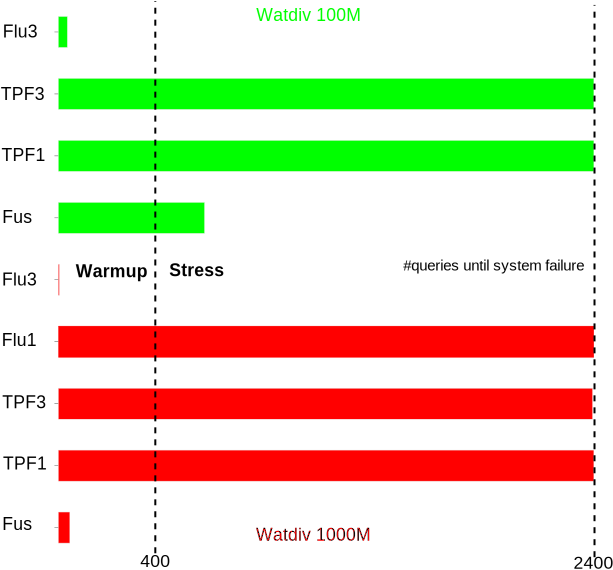
\includegraphics[width=0.99\linewidth]{imgs/F2_BenchmarkSurvival_Other_Reworked}
%	\caption{Benchmark survival for other systems. \textbf{TPF} stays operational for both WatDiv1000M and WatDiv100M. Both as an approach to handle compressed data (\textbf{TPF1})
%		as an approach to support query federation (\textbf{TPF3}) it fulfills its promise of high availability. As of the other approaches only \textbf{Fus} gets passed the warmup phase for WatDiv100M.}
%	\label{fig:F2_BenchmarkSurvival_Other_Reworked}
%\end{figure}
%FIG_ScalingNoSQL
%\begin{figure*}[!ht]
%	\centering
%	\includegraphics[width=0.99\linewidth]{imgs/F6_Scaling_NoSQL_WatDiv1000M_Reworked.eps}
%	\caption{Four panels showing the effect of adding more RAM and \emph{optimized} configurations on the query runtime distribution for WatDiv1000M. In the \emph{optimized} setting Blazegraph and GraphDB share second place. Virtuoso outperforms the other stores even in the 32GB, \emph{default} setup. Adding more memory doesn't impact its performance implying that it doesn't require extra resources. For GraphDB the effect of proper configuration is the most extreme, its performance strongly depends on turning on the correct indexes.}
%	\label{fig:F6_Scaling_NoSQL_WatDiv1000M_Reworked}
%	%\rv{Always name the axes also inside of the figure. I know it's in the caption, but \emph{some} reviewer \emph{will} nag about it.}
%\end{figure*}


\subsection{RFI: Optimized Configurations}
\label{subsec:rfi}
%
%RESULTS Rev1
%RUNTIME
%SUCCESS/ERROR

%Convergence of results? Not with memory, with configs though...
After contacting the vendors with our initial results one of the parties suggested to demonstrate the optimal operation of their database. 
This was formalized by sending out a Request-For-Information (RFI), specifying the benchmarks we were planning to run.
3 out of 4 vendors chose to participate in the RFI, which resulted in an \emph{Optimized} configuration. 

In Figure~\ref{fig:Fig02_WatdivVerticalScaling} the rightmost panel corresponds to running the benchmark with the \emph{Optimized} configuration.

%
%median/mean
%Bla_N1_64_W1000_Def     2.825023 	6.741764
%Gra_N1_64_W1000_Def    40.375218 	59.564284
%Vir_N1_64_W1000_Def     0.175917 	3.667321
%
%Bla_N1_64_W1000_Opt    0.739366 	1.945429
%Gra_N1_64_W1000_Opt    0.652474  	6.320693
%Vir_N1_64_W1000_Opt    0.167420 	4.054050
%
\begin{itemize}
	\item \textbf{Sensitivity to configuration:} \textbf{Vir1\_64} got no benefit from the RFI settings file. For 
	\textbf{Bla1\_64} the only improvement was to explicitly configure the timeout parameter on the server side. This avoids unnecessary overhead while the client is already disconnected. It leads to a speedup of approximately 3.5 for both runtime measurements. \textbf{Gra1\_64} has the highest sensitivity to proper configurations. The provided scripts ensure a batch speedup of 9.4 and a median runtime speedup of 62.
	\item \textbf{32\_Def to 64\_Opt:} Moving from the left panel to the right in Figure~\ref{fig:Fig02_WatdivVerticalScaling}, we clearly see results converging. \textbf{Bla1\_64} is the most efficient system for processing batch workloads with an average runtime of 1.95s per query, 4.05s and 6.32s for \textbf{Vir1\_64} and \textbf{Gra1\_64} respectively. In the query performance \textbf{Vir1\_64} has a median runtime of 0.17s where \textbf{Gra1\_64} and \textbf{Bla1\_64} have runtimes of 0.65s and 0.74s respectively.
%Bla_N1_32_W100_Def   0.191359		0.461707	=> x5
%Gra_N1_32_W100_Def   0.047812		0.417214 	=> x15
%Vir_N1_32_W100_Def   0.046707		0.301350	=> x15
	\item \textbf{Runtime vs Dataset Size:} Returning to section~\ref{subsec:bigdata} we can verify that the linear scaling behavior is largely restored, confirming our earlier hypothesis. Multiplication factors drop to 4.2 for Blazegraph, for Virtuoso and GraphDB mf $ \approx 15$.
\item \textbf{Timeouts \& Errors:} Apart from 5\% timeouts for \textbf{Gra1\_64\_Opt}, no query errors are observed with the \emph{Optimized} configurations.
\end{itemize}
%Bla_N1_64_W1000_Opt:	Success: 100.	Error: 0.0	Timeout: 0.0
%Gra_N1_64_W1000_Opt:	Success: 95.0	Error: 0.0	Timeout: 5.0
%Vir_N1_64_W1000_Opt:	Success: 100.	Error: 0.0	Timeout: 0.0



\subsection{Semantic Web Solutions}
\label{subsec:semweb}
%
%RESULTS Rev1: Notebook Rev1_13 - A Median & Average Runtime
%median/mean
%LdF_N1_64_W100_Def     19.949113	64.842078
%LdF_N3_64_W100_Def     58.365978 	122.960265
%LdF_N1_64_W1000_Def    300.0		219.935204
%LdF_N3_64_W1000_Def    300.0		216.525390
%
%RESULTS Rev1: Notebook Rev1_13 - B Errors & Timeout percentage
%Fus_N1_64_W100_Def:	Success: 65.0	Error: 0.0	Timeout: 34.9
%FedX_N3_64_W100_Def:	Success: 0.0	Error: 0.0	Timeout: 0.0
%LdF_N1_64_W100_Def:	Success: 89.0	Error: 0.0	Timeout: 10.9
%LdF_N3_64_W100_Def:	Success: 75.2	Error: 0.0	Timeout: 24.7
%
%Fus_N1_64_W1000_Def:	Success: 0.0	Error: 0.0	Timeout: 0.0
%FedX_N1_64_W1000_Def:	Success: 95.0	Error: 0.0	Timeout: 5.0
%FedX_N3_64_W1000_Def:	Success: 0.0	Error: 0.0	Timeout: 0.0
%LdF_N1_64_W1000_Def:	Success: 28.8	Error: 0.0	Timeout: 71.1
%LdF_N3_64_W1000_Def:	Success: 29.3	Error: 0.0	Timeout: 70.6
%

%As the initial goal of the research collaboration with Ontoforce was to find a solution to work with federated querying on top of live data sources on the Semantic Web, 
In this section we discuss the results of \textbf{Fus1\_64}, \textbf{FedX3\_64}, \textbf{TPF1\_64} and \textbf{TPF3\_64}. 
For these 3 systems engine failure and query errors are very common with only the \textbf{TPF*\_64} systems surviving the entire benchmark.
Fig.~\ref{fig:Fig03_BenchmarkSurvival_Other_Watdiv_Default} shows the \emph{Benchmark Survival Interval}, defined as the range between the first and the last successful query. 
Given the high degree of failures we do not show the query runtime results.
%Note however that these results do not affect the plots as we only use query events from the \emph{benchmark survival interval}. 
%Fig. deliberately has no relation with query runtimes. 

%Benchmark Survival
%Finally, a subtle error can be made in query runtime comparison for benchmarks which involve a query engine that becomes unresponsive (engine failure). In the runtime comparisons we only consider  We name this the \emph{benchmark survival interval}, this is shown in Figure~\ref{fig:Fig03_BenchmarkSurvival_Other_Watdiv_Default}.

\begin{itemize}
	\item \textbf{FedX1\_64:} This single-node setup is tested to verify whether FedX manages to parse the queries. As the queries have the same form for WatDiv100M we only tested this in the 1000M setting.
	\item \textbf{Specific Templates cause crashes:} Where \\ \textbf{TPF*\_64} systems more gracefully timeout on the \textbf{C} templates, \textbf{C2} causes a crash in \textbf{Fus1\_64} and \textbf{C3} in \textbf{FedX3\_64}, upon their first occurrence in warm-up or stress run. \textbf{C3} is a query with very low triple pattern selectivity leading to large in-memory joins.
	\item \textbf{Crash investigation:} For \textbf{FedX3\_64} the benchmark was terminated after running into constant timeouts for 8 hours. Inspection of the slave nodes showed them to be idle, while the federator node had its entire memory pool saturated, with the CPU load close to zero. This might be related to issues with garbage collection.
	For \textbf{Fus1\_64} after a number of queries a continuous timeout sequence sets in. The specific HDT implementation for Fuseki ignores the timeout parameter. This might explain why the server became unresponsive.
	\item \textbf{Staying alive:} \textbf{TPF*\_64} survive both WatDiv benchmarks, nonetheless with up to 71\% of the queries timeouts on WatDiv1000M. On WatDiv100M the timeout ratio drops to 25\% for \textbf{TPF3\_64} and to 11\% for \textbf{TPF1\_64}.
%Fus_N1_64_W100_Def:	Success: 65.0	Error: 0.0	Timeout: 34.9
%FedX_N3_64_W100_Def:	Success: 0.0	Error: 0.0	Timeout: 0.0
%LdF_N1_64_W100_Def:	Success: 89.0	Error: 0.0	Timeout: 10.9
%LdF_N3_64_W100_Def:	Success: 75.2	Error: 0.0	Timeout: 24.7
%
%Fus_N1_64_W1000_Def:	Success: 0.0	Error: 0.0	Timeout: 0.0
%FedX_N1_64_W1000_Def:	Success: 95.0	Error: 0.0	Timeout: 5.0
%FedX_N3_64_W1000_Def:	Success: 0.0	Error: 0.0	Timeout: 0.0
%LdF_N1_64_W1000_Def:	Success: 28.8	Error: 0.0	Timeout: 71.1
%LdF_N3_64_W1000_Def:	Success: 29.3	Error: 0.0	Timeout: 70.6
	\item \textbf{Runtime Comparison: } Only for WatDiv100M comparing the runtimes of \textbf{TPF*\_64} to the \emph{Vendor} systems is meaningful due to the higher query success rates. Compared to \textbf{ES1\_32}, the \textbf{TPF1\_64} is 2.4 times faster in terms of median runtime and 12\% in terms of average runtime. For \textbf{TPF3\_64} the results are worse than \textbf{ES1\_32}: 25\% slower in median runtime, 40\% slower for average runtime.
\end{itemize}
%Bla_N1_32_W100_Def   0.191359		0.461707
%Gra_N1_32_W100_Def   0.047812		0.417214
%Es_N1_32_W100_Def    48.305706		72.994550
%Vir_N1_32_W100_Def   0.046707		0.301350
%LdF_N1_64_W100_Def     19.949113	64.842078
%LdF_N3_64_W100_Def     58.365978 	122.960265











\subsection{Horizontal scaling}
\label{subsec:hscaling}
%
%RESULTS Rev1: Notebook Rev1_13 - A Median & Average Runtime
%
%median/mean
%Vir_N1_32_W1000_Def    0.295139	4.431931
%Vir_N3_32_W1000_Def    1.040609	8.545433
%
%Es_N1_32_W1000_Def     74.091186 	132.011802
%Es_N3_32_W1000_Def    300.000000 	191.478380
%   
%LdF_N1_64_W1000_Def    300.0 		219.935204
%LdF_N3_64_W1000_Def    300.0		216.525390
%
%RESULTS Rev1: Notebook Rev1_13 - B Errors & Timeout percentage
%Bla_N1_32_W10_Def:	Success: 100.	Error: 0.0	Timeout: 0.0
%Gra_N1_32_W10_Def:	Success: 100.	Error: 0.0	Timeout: 0.0
%Es_N1_32_W10_Def:	Success: 100.	Error: 0.0	Timeout: 0.0
%Vir_N1_32_W10_Def:	Success: 100.	Error: 0.0	Timeout: 0.0
%
%Bla_N1_32_W100_Def:	Success: 100.	Error: 0.0	Timeout: 0.0
%Gra_N1_32_W100_Def:	Success: 100.	Error: 0.0	Timeout: 0.0
%Es_N1_32_W100_Def:	Success: 100.	Error: 0.0	Timeout: 0.0
%Vir_N1_32_W100_Def:	Success: 100.	Error: 0.0	Timeout: 0.0
%
%Bla_N1_32_W1000_Def:	Success: 88.3	Error: 0.0	Timeout: 11.6
%Gra_N1_32_W1000_Def:	Success: 100.	Error: 0.0	Timeout: 0.0
%Es_N1_32_W1000_Def:	Success: 67.2	Error: 0.0	Timeout: 32.7
%Vir_N1_32_W1000_Def:	Success: 99.9	Error: 0.04	Timeout: 0.0
%
%Bla_N1_64_W1000_Def:	Success: 95.0	Error: 0.0	Timeout: 5.0
%Gra_N1_64_W1000_Def:	Success: 79.6	Error: 0.0	Timeout: 20.4
%EsS_N1_64_W1000_Def:	Success: 72.5	Error: 0.0	Timeout: 27.4
%Vir_N1_64_W1000_Def:	Success: 100.	Error: 0.0	Timeout: 0.0
%
%Bla_N1_64_W1000_Opt:	Success: 100.	Error: 0.0	Timeout: 0.0
%Gra_N1_64_W1000_Opt:	Success: 95.0	Error: 0.0	Timeout: 5.0
%Vir_N1_64_W1000_Opt:	Success: 100.	Error: 0.0	Timeout: 0.0
%
%Es_N3_32_W1000_Def:	Success: 34.8	Error: 65.1	Timeout: 0.0
%Vir_N3_32_W1000_Def:	Success: 100.	Error: 0.0	Timeout: 0.0
%
%Fus_N1_64_W100_Def:	Success: 65.0	Error: 0.0	Timeout: 34.9
%Flu_N3_64_W100_Def:	Success: 0.0	Error: 0.0	Timeout: 0.0
%LdF_N1_64_W100_Def:	Success: 89.0	Error: 0.0	Timeout: 10.9
%LdF_N3_64_W100_Def:	Success: 75.2	Error: 0.0	Timeout: 24.7
%
%Fus_N1_64_W1000_Def:	Success: 0.0	Error: 0.0	Timeout: 0.0
%Flu_N1_64_W1000_Def:	Success: 95.0	Error: 0.0	Timeout: 5.0
%Flu_N3_64_W1000_Def:	Success: 0.0	Error: 0.0	Timeout: 0.0
%LdF_N1_64_W1000_Def:	Success: 28.8	Error: 0.0	Timeout: 71.1
%LdF_N3_64_W1000_Def:	Success: 29.3	Error: 0.0	Timeout: 70.6
%
%Bla_N1_64_Ont_Opt:	Success: 0.0	Error: 0.0	Timeout: 0.0
%Es_N1_64_Ont_Def:	Success: 57.6	Error: 22.2	Timeout: 20.0
%Gra_N1_64_Ont_Opt:	Success: 45.0	Error: 0.0	Timeout: 54.9
%Vir_N1_64_Ont_Opt:	Success: 98.7	Error: 0.67	Timeout: 0.58
%Vir_N1_32_Ont_Opt_VWall:	Success: 98.8	Error: 0.67	Timeout: 0.50
%Vir_N3_64_Ont_Opt_0:	Success: 95.8	Error: 3.71	Timeout: 0.45
%Vir_N3_64_Ont_Opt_2:	Success: 86.0	Error: 13.9	Timeout: 0.0
%
%


An alternative to increasing the memory in a single-node server is to increase the overall resources by 
adding more nodes, thus creating a distributed system. 

All 4 commercial RDF solutions support multi-node setups. GraphDB however, works only as a HA-solution (High-Availability): we did not evaluate this approach since 
it requires all data to be replicated on every node and does not support data partitioning, which is required to scale beyond the single-node resource limits.
The performance can however be estimated since it is equivalent to a setup with N identical databases with a load balancer equally distributing the queries between
the database replicas. The effect is a linear speedup in terms of completing a full query-mix. 
Virtuoso also supports a similar setup.
The effect on the individual query runtimes should be limited, but not completely absent since the database load on the individual nodes will be smaller. The effect of database load on the query runtimes will be studied in the next section.


For Blazegraph, support was required for setting up the multi-node system. This support was requested via the RFI but not fulfilled, which limited our comparison to \textbf{Vir3\_32\_Def}, \textbf{ES3\_32\_Def}, and \textbf{TPF3\_64\_Def}.

Fig.~\ref{fig:Fig04_WatdivHorizontalScaling} shows pairwise comparisons of the three setups for which we have both a single and a 3-node benchmark. 

\begin{itemize}
	\item \textbf{Benchmark survival interval:} %[('ES_N3_32_W1000_Def', 8684), ('Vir_N3_32_W1000_Def', 12000)]
	\textbf{Vir3\_32\_Def} and \textbf{TPF3\_64\_Def} managed to stay online during the entire Watdiv1000M benchmark, whereas \textbf{ES3\_32\_Def} stopped responding after having completed 67\% of the multi-threaded run. 
	%Es_N3_32_W1000_Def:	Success: 34.8	Error: 65.1	Timeout: 0.0
	%Vir_N3_32_W1000_Def:	Success: 100.	Error: 0.0	Timeout: 0.0
	\item \textbf{Errors \& Timeouts:} 65\% of the queries of \textbf{ES3\_32\_Def} resulted in an HTTP 504 error, mentioning \textit{Gateway Timeout}. Further study revealed that this timeout was due to an internal configuration parameter in the ES distributed setup, unfortunately we did not receive any feedback on this issue. \textbf{Vir3\_32} successfully completed all queries. 70.6\% of the queries result in a timeout for \textbf{TPF3\_64\_Def}.
	\item \textbf{Multi-node overhead:} For all setups additional nodes lead to overhead instead of speedup. Runtime MFs are 1.9 and 1.5 for \textbf{Vir} and \textbf{ES}. \textbf{TPF} has a negligible overhead but is already very close to the query timeout.
\end{itemize}
%query_events_correct => double check on crash!
%Es: (Virtuoso 12k = all, TPF_64 also all)
% T1 warmup survival: 	2000
% T stress: 1343 - 1331 - 1348 - 1320 - 1348
%median/mean
%Vir_N1_32_W1000_Def    0.295139	4.431931
%Vir_N3_32_W1000_Def    1.040609	8.545433
%
%Es_N1_32_W1000_Def     74.091186 	132.011802
%Es_N3_32_W1000_Def    300.000000 	191.478380
%   
%LdF_N1_64_W1000_Def    300.0 		219.935204
%LdF_N3_64_W1000_Def    300.0		216.525390

In a discussion with OpenLink it was clarified that Virtuoso Cluster acts as a \emph{distributed memory solution}. This implies that adding nodes does not lead to a speedup in the query runtimes, but the total of memory pool in the system increases, allowing it to handle larger datasets. Since the single node benchmark did not exhaust the memory, there is no advantage to be expected from a multi-node setup. As an indication, according to support a 32GB machine should be able to manage up to 3 billion triples (10GB per 1B triples). 
This observation, together with the lack of feedback on the issues with \textbf{ES3\_32\_Def} and the high timeout percentage for \textbf{TPF3\_64\_Def} motivated our decision to not run any further multi-node benchmarks..

Systems translating SPARQL queries to distributed platforms such as Hadoop~\cite{cure2015evaluation, graux2016multi} are an alternative approach we did not test. Although these approaches are usually not recommended in a context with low-latency requirements, they are specifically designed to operate in an ETL-setting. 
Results for S2RDF~\cite{Schatzle:2016:SRQ:2977797.2977806}, which uses Apache Spark on Watdiv1000M indicate that a 10-node setup can be close to 10 times faster than a single-node Virtuoso server. Since these SPARQL-on-Hadoop solutions are not sufficiently mature and for example cannot be tested using a SPARQL endpoint, definite conclusions currently can not be drawn. 
%One observation to motivate this caution is the fact that Virtuoso is hardly affected when running multiple benchmark clients at once, as will be shown in section~\ref{subsec:load}. The operational cost for these Hadoop setups can also not immediately be deduced.

















\section{Results II: Query Runtime Analysis in Depth}
\label{sec:runtimefactors}
Only comparing query runtimes might be an oversimplification in benchmark analysis. 
When comparing the average runtimes of a batch of queries the slow tail of the distributions dominates have the largest impact on the result. In the first subsection
%~\ref{subsec:templates} 
we investigate whether certain query templates dominate the average runtimes.
Query execution times depend on the state of the database, which motivates studying the query context. Previous results are still valid as all queries are executed 5 times and each time the median is taken to calculate average runtimes.

The next subsection
%~\ref{subsec:load} 
studies the effect of the server load on the query runtimes by comparing a single-client benchmark with a stress test with 5 clients. In the following subsection we investigate the context of a query by studying caching effects. 

%This will be explored in section~\ref{subsec:caching}. 
We conclude by studying an often unreported effect: result completeness can have a big impact on the query runtimes and should always be verified.
%as we will discuss in section~\ref{subsec:completeness}.

\subsection{Query runtimes for different template types}
\label{subsec:templates}

%
%RESULTS Rev1: Notebook Rev1_14

%Bla_N1_64_W1000_Opt Gra_N1_64_W1000_Opt ES_N1_64_W1000_Def Vir_N1_64_W1000_Opt LDF_N1_64_W1000_Def
%template_type 					
%C 	10.953371 	33.118651 	300.000000 	29.163331 	300.0
%F 	0.710602 	1.041088 	112.866074 	0.551893 	300.0
%L 	0.567620 	1.054375 	25.129921 	0.191519 	300.0
%S 	0.634281 	0.427514 	26.836085 	0.083854 	300.0
%
%
%
%Bla_N1_64_W1000_Opt Gra_N1_64_W1000_Opt ES_N1_64_W1000_Def Vir_N1_64_W1000_Opt 	LDF_N1_64_W1000_Def
%template 					
%C1 	4.853528 	41.074082 	300.000000 	50.148527 	300.000000	Bla
%C2 	17.724176 	25.320613 	300.000000 	10.052103 	300.000000	Vir
%F1 	0.651362 	0.590807 	10.350239 	0.064754 	300.000000	Vir
%F2 	0.769873 	1.529352 	133.287122 	4.005216 	300.000000	Bla
%F3 	1.176846 	2.933791 	300.000000 	4.955930 	300.000000	Bla3
%F4 	0.887820 	4.861341 	300.000000 	0.668484 	300.000000	Vir
%F5 	0.064486 	0.060477 	2.468437 	0.019201 	6.090464	Vir
%L1 	0.035158 	0.006558 	1.346970 	0.007135 	2.848204	Vir
%L2 	1.650052 	2.166173 	25.129921 	0.302525 	300.000000	Vir
%L3 	0.037243 	0.009755 	1.025530 	0.006762 	2.260012	Vir
%L4 	0.791782 	4.210585 	51.241839 	0.370861 	300.000000	Vir
%L5 	1.185084 	4.131350 	122.003833 	0.317177 	300.000000	Vir
%S1 	0.046855 	0.011460 	3.790836 	0.137013 	4.298328	Gra
%S2 	0.941007 	2.177947 	46.095154 	0.160746 	300.000000	Vir
%S3 	1.636567 	0.445906 	26.885182 	0.069650 	300.000000 	Vir
%S4 	0.670550 	0.411107 	81.268466 	0.084230 	300.000000	Vir
%S5 	1.026515 	0.458653 	300.000000 	0.070567 	300.000000	Vir
%S6 	0.206022 	0.141913 	7.889212 	3.760982 	300.000000  Gra
%S7 	0.037128 	0.005170 	0.295254 	0.005701 	0.945705	Gra3
%\caption{Average Runtime per query template for 5 single-node setups. \textbf{TPF1\_64} has only 5 templates which do not coincide with the timeout of 300s, for \textbf{ES1\_64\_Def} this is alread 15 templates.
%\textbf{Vir1\_64\_Opt} is the fastest engine for 13 templates, \textbf{Gra1\_64\_Opt} for and \textbf{Bla1\_64\_Opt} for 3 templates each. Template \textbf{C3} was omitted due to query completeness issues. Blazegraph was the only engine to retrieve all results. } 
The queries of the WatDiv benchmarks are all BGPs but have different shapes and selectivity properties. The benchmark generator has 20 templates which can be further organized into 4 template categories (shapes). 
In Figure~\ref{fig:Fig06_WatdivTemplateTypes} we show the average runtime per template for 5 stores on WatDiv1000M.
\begin{itemize}
	\item \textbf{Template timeouts:} For \textbf{TPF1\_64} 15 runtime averages coincide with the benchmark timeout (300s). Successful queries are spread out over the different types: \textbf{F}:1, \textbf{S}:2, \textbf{L}:2.
	\textbf{ES1\_64\_Def} has timeouts for the 2 \textbf{C} queries,  2 \textbf{F} queries, and 1 \textbf{S} query. The other stores have no averages close to timeout.
	
	\item  \textbf{Template winners:} \textbf{Vir1\_64\_Opt} is the fastest engine for 13 templates, nonetheless \textbf{Bla1\_64\_Opt} was better on batch workloads. These workloads are dominated by the runtimes of the \textbf{C}-templates, more specifically \textbf{C1} seems to explain the difference. 
	\textbf{Gra1\_64\_Opt} performs best for 3 \textbf{S}-templates, \textbf{Bla1\_64\_Opt} wins on 1 \textbf{C}- and 2 \textbf{F}-templates. Template \textbf{C3} was omitted due to query completeness issues. Blazegraph was the only engine to retrieve all results within the timeout boundary.
	\textbf{Vir1\_64\_Opt} wins: \textbf{C}:1, \textbf{F}:3, \textbf{S}:4, and all \textbf{L}-templates.
\end{itemize}

If we generalize further and only distinguish between 4 query template types, as can be seen in Figure~\ref{fig:Fig06_WatdivTemplateTypes}, it becomes even more apparent where the difference between Blazegraph and Virtuoso can be situated: the \textbf{C}-templates.
\begin{itemize}
	\item \textbf{Ranking per template type:} This pattern is very stable, \textbf{Vir1\_64\_Opt} first, followed by \textbf{Bla1\_64\_Opt} and \textbf{Gra1\_64\_Opt}. Only for \textbf{C}-templates Blazegraph has the advantage  by a factor 3: 10s vs 30s. The differences on the other templates are lower by an order of magnitude, each time in the range of 0.2 - 0.5 seconds. For the \textbf{S}-templates GraphDB performs slightly better than Blazegraph.
	\item \textbf{Engine specialities:} For Blazegraph the \textbf{C}, \textbf{F}, and \textbf{S}-templates result in similar runtimes. GraphDB has a small preference to \textbf{S}-templates. Virtuoso is much better than the competition for \textbf{L}-queries and \textbf{S}. For the \textbf{F}-template all three engines perform similarly.
\end{itemize}

\subsection{Single versus Multi-client stress testing}
\label{subsec:load}

%
%RESULTS Rev1: Notebook Rev1_11 
%results
%1T vs 5T are the runtime of the MEAN query!
%5T runtime corresponds to the max runtime of a query in the stress test, 1T is the runtime during the warmup phase, 5T was chosen max to try and suppress caching effects, therefore fluctuations might be mainly attributed to gaussian noise
%FIGure Caption
%Runtimes for single versus multi-client workloads: 1 vs. 5 threads. 
%5T runtime corresponds to the maximum runtime per query in the stress test, 1T is the runtime during the warmup phase. The red line corresponds to the bisector, where the runtime for both workloads is equal. Dots are expected to be shifted up, which correspond to a multiplication factor. The closer the dots to the bisector the smaller the multi-client overhead. Dots below the bisector can be attributed to the natural variance in query runtimes. Average runtimes per store are also shown. \textbf{Bla1\_64} and \textbf{Vir1\_64} have the smallest overhead $(< 20\%)$, for \textbf{ES1\_64} has the largest $(> 300\%)$.
All results so far focused on the multi-threaded benchmark run, in which 5 benchmark clients are simultaneously executing the same query-mix in a (different) randomized order. It is however interesting to take into account the effect of server load. In Figure~\ref{fig:Fig07_Watdiv_SingleMultiClient} we compare, per query, the runtime of the single-threaded warm-up run versus the runtime of the slowest multi-threaded run. We chose the slowest query as this has the highest probability of eliminating the effects of caching which will be studied in the next section. Note that for the \emph{SemWeb} systems the comparison is on WatDiv100M, while the \emph{Vendor} systems are compared on WatDiv1000M.

%Bla, Gra, ES, Vir, Fus, TPF1, TPF3
%11.7	10.4		1.125
%8.3	3.93		2.1119592875
%72.4	17.2		4.2093023256
%4.53	3.78		1.1984126984
%65		46.5		1.3978494624
%54.1	30.8		1.7564935065
%90.8	47.4		1.9156118143

\begin{itemize}
	\item \textbf{Highest resilience against server loads}: The lowest multiplication factors (mf) are 1.1 , 1.2, and 1.4 for \textbf{Vir1\_64\_Opt}, \textbf{Bla1\_64\_Opt}, and \textbf{Fus1\_64\_Def} respectively. 
	 
	\item \textbf{Lowest resilience against server loads:} For \textbf{TPF*\_64\_Def} the mf is 1.8 - 1.9.  \textbf{Gra1\_64\_Opt}'s mf is at 2.1, but for \textbf{ES1\_64\_Opt} we have an mf of 4.2.
	
	\item \textbf{Variance of query runtimes:} For Blazegraph and GraphDB the larger variance on the query runtimes might still be explained as being the result of caching. As we will see in the next section however, we don't observe caching effects for GraphDB and for Blazegraph we only see a weak effect for the slow-running queries (\textbf{C}-templates).
\end{itemize}


\subsection{The Role of Caching in Query Runtime Results}
\label{subsec:caching}
%
%RESULTS Rev1: Notebook Rev1_08 and Rev1_09 
%TODO study number is notebook 09

%RESULTS ORIGINAL PAPER
%NONE


Some data stores cache the results of queries. Especially in a benchmark where the same query is executed multiple times, this might lead to a large variance on the query runtimes. Although the approach with query events was not designed with support for studying caching effects in mind, having the order of the queries suffices. 
In an initial attempt we plotted the query runtimes as a function of the distance to their nearest preceding execution. For this distance we experimented with the number of intermediary queries, the total number of intermediary results, and the amount of time in between. Results were very similar but did not show any clear pattern. 
In Figure~\ref{fig:Fig08_Watdiv_caching} however, the speedup with respect to the slowest query execution in the multi-client run is plotted as a function of the actual query runtime. This visualization allows an easy distinction between speedups which are caused by noise, mainly for very short query runtimes, and real caching effects. If no caching effects are present the plot should have all its dots on the X and Y-axis.
%Fig. 8. Speedup in query runtime by comparing all query runtimes in the multi-threaded run with the slowest execution in the stress test. With
%no caching all dots are expected on the X and Y-axis, the latter because of the noise on small query runtimes. If we focus on speedups > 2,
%especially ES1 and TPF* seem to have the highest benefit.
\begin{itemize}
	\item \textbf{Stores with a clear caching advantage:} The \textbf{TPF} server instances have NGINX~\cite{nginx} cache enabled. The similarity in results with other stores strengthens the idea that Figure~\ref{fig:Fig08_Watdiv_caching} in fact shows caching behavior for \textbf{TPF*\_64}, \textbf{ES1\_64\_Doc}, and \textbf{Gra1\_64\_RFI}.
	
	\item \textbf{Caching differences per template type:} For \textbf{ES1\_64\_Doc} and \textbf{Gra1\_64\_RFI} the \textbf{F}-templates (blue) dots correspond to the highest speedups. For \textbf{TPF*\_64} query execution is in general slower than for the other systems, therefore \textbf{L} and \textbf{S}-queries, shift to the right and their speedups become more prominent. Small speedups for \textbf{Bla1\_64} and \textbf{Vir1\_64} are mostly limited to the \textbf{C}-template queries.
	\item \textbf{TPF1 vs TPF3:} As a result of the horizontal data partitioning scheme \textbf{S} and \textbf{F}-queries can be resolved locally for \textbf{TPF3\_64}, which explain the higher prevalence in the plot.
\end{itemize}












\subsection{Query Result Completeness}
\label{subsec:completeness}

In our SWAT4LS contribution~\cite{dewitte_swat4ls_2016} we discovered that query runtimes cannot be trusted without paying careful attention to query completeness. We revisited earlier results on WatDiv and discovered some inconsistencies as well.
\begin{itemize}
	\item \textbf{Vir*\_Doc:} Running Virtuoso with the \emph{Documented} configurations gave it an advantage since in this setting the result count is limited to $100,000$. This only affects the \textbf{C3} queries for all sizes of WatDiv.
	\item \textbf{Vir*\_RFI:} \textbf{Bla1\_64\_RFI} was the only engine to correctly solve all \textbf{C3} templates. This query returns the highest number of results: 42,063,279. Although Virtuoso was configured to report an unlimited number of results, we discovered that for multiple independent queries the result count is limited to the magic number: 1,048,576. (which is $2^{20}$).  
\end{itemize}
As was mentioned in the introduction of section~\ref{sec:tradeoffs}, none of the runtime results reported so far are affected by this query incompleteness: we discarded all queries for which at least one store had a different number of results as compared to the consensus. In practice this means that all \textbf{C3} queries had to be discarded. The impact on the runtime comparisons is big as \textbf{C3} has the highest runtimes and ignoring query completeness would put Blazegraph at a serious disadvantage.


\section{Results III: Real-world Life Sciences Benchmark Results}
\label{sec:realworld}


%waarom uitleggen
% in store preselection staat het volgende:
%The comparison with these SemWeb systems was an essential part of the research collaboration with Onto-
%force as their initial goal was to build their DISQOVER search interface on top of a federated querying system.
%The advantage of the latter is that their interface would then provide a live view on a continuously updating
%Life Sciences Linked Data cloud, removing the need for an ETL process.
As was explained in section~\ref{subsec:featurematrix}, the WatDiv benchmark and the Ontoforce benchmark are related. The Ontoforce benchmark consists of interactive federated queries which are extracted from the user logs of the DISQOVER product. These queries are currently solved by combining an ETL preprocessing step, which integrates the different Life Sciences datasets offline using Ontoforce's own central ontology. This ETL step bares a lot of similarity with the WatDiv benchmark as it consists of mostly BGP queries. The queries of the Ontoforce benchmark are the result of faceted browsing, whereby, in practice, the facet filters are performed by a distributed search system (SOLR), but their product can also run with a SPARQL-based back-end. In this section we evaluate the ability of \emph{Vendor} systems to work with these types of queries and therefore serve as an alternative to a search system.

%Runtimes - minder belangrijk, meer focus op waarom
%N1_64_Opt Ontoforce => for both ES and Virtuoso no response time <> runtime
%Blazegraph crashed
%Es 380848.276950983	380849.972397525				=> coincide
%GraphDB crashed
%23258.549703492	23261.613780134						=> coincide
The Ontoforce benchmark has a very challenging query set. Therefore the focus of section~\ref{sec:realworld} will be far less on query runtimes but more on trying to extract insights which are generalizable. In this benchmark run the response times consistently coincide with the query runtimes.  
%More challenging => meer errors => besproken in aparte sectie
In section~\ref{subsec:erroranalysis} we give more detailed insights in the behavior of the different systems on the Ontoforce benchmark. We pay special attention to query failures and query completeness.
In section~\ref{subsec:dtrees} we try to automatically extract the reasons behind query success, failure, different error types, and slow versus fast running queries. This automation is achieved by making use of decision tree analysis.
Finally, in section~\ref{sec:bmcost} we compare the results of all benchmarks in this research using \emph{Benchmark Cost} as a unification parameter. This allows to make comparisons between setups which are very different in nature and see whether the trends in the benchmark results are consistent. This approach also takes into account the cost for data ingestion and the different licensing fees.


\subsection{Benchmark Error Analysis}
\label{subsec:erroranalysis}
%
%RESULTS Rev1: Notebook Rev1_02  

%exacte cijfers over timeouts en aantal error in data notebook
%Crosstabs (ALL warmup & stress):	Success	Unverified	Incomplete	Timeout Error Unknown (all = 7338)
%Bla_N1_64_Ont_Opt 					36		0			0			431		0	  6871 (94%) 	
%Es_N1_64_Ont_Def 					4246	0			4			1257	1830  ALL 	
%Gra_N1_64_Ont_Opt 					1583	0			0			2372	0	  3383 (46%)	
%Vir_N1_64_Ont_Opt 					7069	120			60			41		48		ALL 	
%Vir32 first test on AWS => 2946 errors! (0 results while consensus > 0) => 41%
%new Vir32 OK same results as Vir64
%Vir64 Incomplete = 6 x 10 queries (<1%) => 1 query incomplete (2^20) andere 0 results terwijl consensus > 0

%Vir3_64_0	many errors but most queries solved at least once => 1122 queries in stres test with at least one susccesful run!
%Vir_N3_64_Ont_Opt_0 				4072	38			27			19		3182		ALL 	
%Vir_N3_64_Ont_Opt_2 				3918	66			2718		0		636			ALL 	
%Reruns telkens maar 100 queries until crash

%TODO notebook contains more info on query correctness

%RESULTS ORIGINAL PAPER
%BMSurvival: 
%	[('Bla_N1_64_Ont_Opt', 55), ('Gra_N1_64_Ont_Opt', 2541), ('ES_N1_64_Ont_Def', 7335), ('Vir_N1_64_Ont_Opt', %7338)]
%ERROR frequency per query
% 						Fail_always	Fail_never 		Fail_sometimes 	Unknown 	thread_type
% 	Bla_N1_64_Ont_Opt 	18 			37 				0 				1168 		warmup
% 	ES_N1_64_Ont_Def 	499 		724 			0 				0 			warmup
% 	Gra_N1_64_Ont_Opt 	233 		988 			0 				2 			warmup
% 	Vir_N1_64_Ont_Opt 	14 			1209 			0 				0 			warmup
%
% 	Bla_N1_64_Ont_Opt 	0 			0 				0 				1223 		stress
% 	ES_N1_64_Ont_Def 	289 		238 			696 			0 			stress
% 	Gra_N1_64_Ont_Opt 	400 		313 			150 			360 		stress
% 	Vir_N1_64_Ont_Opt 	15 			1208 			0 				0 			stress
%GraphDB fails after completing 21\% of the stress test.
%Virtuoso is consistent and successful in 99\% of the queries, ES survived benchmark and is consistently successful for 59\% and 19\% of the queries during %warmup and stress run respectively.
 %[('Vir_N3_64_Ont_Opt_0', 4313), ('Vir_N3_64_Ont_Opt_1', 179), ('Vir_N3_64_Ont_Opt_2', 7338), ('Vir_N3_64_Ont_Opt_AWS1', 116), ('Vir_N3_64_Ont_Opt_AWS2', 224), ('Vir_N3_64_Ont_Opt_AWS3', 228)]



\paragraph{Error Frequencies}

The \emph{Prototypes} and \textbf{Vir*} have been tested on the Ontoforce benchmark for our SWAT4LS~\cite{dewitte_swat4ls_2016} contribution. Note that \textbf{TPF} systems do not currently support all SPARQL operators and could therefore not be run on this benchmark.  In Figure~\ref{fig:Fig09_FailuresOntoforceBM} we show the results for the \emph{Vendor} systems. Each simulation consists of a small bar, corresponding to the single-threaded warm-up run, and 5 concatenated bars corresponding to 5 threads in the stress test.
The Figure also shows that only Virtuoso simulations had a sufficiently wide benchmark survival interval to enable further analysis.

\begin{itemize}
	\item \textbf{Bla1\_64\_Opt:} One major difference with the results on the WatDiv benchmark is Blazegraph's inability to handle the complexity of the Ontoforce queries, resulting in very short benchmark survival interval: it contains only 55 queries, of which 18 are timeouts.
	
	\item \textbf{Gra1\_64\_Opt:} GraphDB also did not survive the entire benchmark, but managed to stay up for 21\% of the stress run. During the stress run it solved 40\% of the queries successfully, the other queries resulted in a timeout. For 38\% of the queries, at least one successful run is available in the stress run.

	\item \textbf{ES1\_64\_Def:} ES was definitely the least successful on the WatDiv benchmarks, but is the only store, apart from Virtuoso, for which the benchmark survival interval spans the entire benchmark. 58\% of the queries were executed successfully. The remainder consists of 25\% HTTP errors and 17\% timeouts. 
%%Vir_N1_64_Ont_Opt 	7069	120			60			41		48		ALL 		
	\item \textbf{Vir1\_*\_Opt:} Virtuoso is both consistent and successful on this benchmark with only 1\% of queries consistently failing, overall the success rate is 98\%. These failures correspond mainly to queries which contain \emph{property paths}. None of the other stores could handle these queries. 
	It should be noted that during the creation of the DISQOVER product, Virtuoso was frequently used as a back-end system, which partially implies a certain favorable bias in the Ontoforce results.The \textbf{Vir1\_32\_Opt} in the SWAT4LS~\cite{dewitte_swat4ls_2016} paper had 41\% incomplete queries. This re-run however, achieves the same figures as the 64GB run.
	
	\item \textbf{Vir3\_64\_Opt\_*:} The  \textbf{Vir3\_64\_Opt} setup was re-run multiple times, the different runs are identified with an additional sequence number 0-2:
	Although the success rate of \textbf{Vir3\_64\_Opt\_0} is only 55\%, 92\% of the queries are successfully executed at least once, which makes it possible to make runtime comparisons. \textbf{Vir3\_64\_Opt\_2} has far less reported errors. Post-processing revealed issues with query completeness (orange) for 37\% of the queries.
\end{itemize}


 
\paragraph{Query Correctness.}

Previously published results~\cite{dewitte_swat4ls_2016} had counter-intuitive runtime results:  \textbf{ Vir1\_32} and \textbf{Vir3\_64\_Opt\_2} executed much faster than \textbf{Vir1\_64}. 
Consequently, we studied the number of results per query:

 
\begin{itemize}
	\item \textbf{Inter-thread consistency:} As a first step we analyzed whether for each individual system the number of query results was consistent for each query-mix. 
	Without any exception this inter-thread consistency was confirmed.
	
	\item \textbf{Query consensus:} In the query event format, described in Table~\ref{table:queryevents}, one field indicates whether a query is correct or its result count incomplete. These values are obtained by creating a query consensus, with the following rules. If at least two separate \emph{Vendor} systems agreed on the number of results we assume this results is `correct', for 97.3\% this is the case. If only 1 engine can solve a query we label these as `uncertain'. Virtuoso solves 19 queries for which no consensus can be derived. For 13 queries none of the systems managed to generate a solution. 8 of these contain a property path operator, the other 5 have \sql{FILTER IN} operators containing large URI lists, such that the file size of the query is between 10 and 100 kb.
	
	\item \textbf{Count Queries:} Of the 19 `uncertain' queries solved by Virtuoso 15 are \sql{count} queries. However, upon inspection the \sql{count} operator was always part of a sub-query, so this result can not be disproven. The benchmark software only reports the number of results per query. We extended it to also download the actual results to be able to verify whether the \sql{count} queries are consistent between the stores. However, no inconsistencies were found there.
	
	\item \textbf{Incorrect Query results:} Some of the Virtuoso benchmarks have incorrect results. The typical pattern is that the query is executed $< 1s$ and generates 0 results. 1 query also had the query result limit $ = 2^{20}$. To get more insight into the context of incomplete queries we executed the \textbf{Vir3\_64} benchmark an additional 3 times. In these runs the incorrect query results were not observed, but, but the new benchmarks never made it to the stress test, with the best run having a benchmark survival interval with a length of 228 queries.
\end{itemize}








\subsection{Decision Tree Analysis of Query Features}
\label{subsec:dtrees}
\begin{table*}[htbp!]
	\centering
	\caption{Query Features and information on their range and correlations with other (discarded) features.}
	\label{table:features}
	%\scalebox{0.9}{
	\begin{tabular}{l|llll}
		\hline
		\textbf{Feature} & \textbf{Prefix} & \textbf{Value} & \textbf{Range} & \textbf{Correlations} \\
		\hline
		\sql{order}       & ORD     & frequency  & [0,1]   & \sql{limit}(0.88) \\
		\sql{filter in}   & FIL\_IN & frequency  & [0,16]  & \sql{union}(0.95), FS(0.95) \\			
		\sql{filter}      & FIL     & frequency  & [0,27]  & tp\_???(0.96), TP(0.95) \\
		\sql{count}       & CNT     & frequency  & [0,1]   & \sql{distinct}(1.0) \\
		Triple Patterns   & TP      & frequency  & [1,38]  & \sql{filter}(0.95) \\
		\sql{graph}       & GRA     & frequency  & [0,1]   & - \\
		\sql{optional}    & ORD     & frequency  & [0,9]   & - \\
		\sql{group}       & GRP     & frequency  & [0,4]   & - \\
		(sub)Queries      & Q       & frequency  & [1,10]  & \sql{union}(0.94), \sql{filter in}(0.94) \\
		file size         & FS      & kilobyte  & 1, 10, 100  & \sql{filter in}(0.97), \sql{union}(0.95) \\
		query engine      & -      &  \emph{Vendor}  & -  & - \\
		\hline
	\end{tabular}
	%}
\end{table*}




%

%	\caption{Decision Tree Analysis to identify the reason for query failure, certain error types, and high/low query runtimes. Input for all trees are feature vectors which represent the frequencies of operators and some structural features such as the amount of sub-queries. Also the query engine is added as a categorical feature. Rules in the decision trees are shown in red, sample sizes are encoded as the width of the bottom bar and the value is added inside the bars in bold. For each separate part the class distribution or the average runtime is reported below the bar. \\ 
%		\textbf{Top:} Classification into query success (blue) and failure (red) and incomplete.  
%		The query engine is an important decision rule, which demonstrates that Virtuoso behaves very different from the other systems. For those (left hand side), the amount of sub-queries (Q) and \sql{optional}s play a big role in predicting query failure. \\
%		\textbf{Center:} Classification of query failures into classes incomplete (orange), server error (green), and timeout (purple). \textbf{Gra1} and \textbf{Bla1} only have timeouts. \textbf{ES1} has a large fraction of HTTP errors as well. \\
%		\textbf{Bottom:}  Regression on query runtimes. Red corresponds to high query runtimes, white to low. For \textbf{Vir1} the amount of \sql{filter in} and \sql{group} (GRP) operators are the most important factors. \textbf{Gra1} seems to run slower for queries containing \sql{filter} (FIL) operators. For the other two systems the presence of \sql{filter in} affects the runtimes negatively.
%		\\
%	}




Ontoforce has released the queries for this benchmark run. However, the queries are very complex and sometimes they take up 1 - 100 kb in disk space. To gain a deeper understanding into why queries fail, have timeouts and HTTP errors, why they are fast or slow to execute,... we created a set of features per query and fitted a decision tree~\footnote{\scriptsize \url{http://scikit-learn.org/stable/modules/tree.html}} to the data. The 3 resulting trees are shown in Figure~\ref{fig:Fig10_AllTrees}. The input features for this algorithm are limited by removing highly correlated features. For example \sql{order} and \sql{limit} are highly correlated. The list of retained query features is given in Table~\ref{table:features} together with the highest correlated operators.
By adding `Query Engine' as an additional feature we can train the decision tree on all the available query event data for the Ontoforce Benchmark. 
\begin{itemize}
	\item \textbf{Dominant Feature:} The `Query Engine' is the most important factor to segment the data in all 3 cases. The absence of this feature would in fact indicate that all systems have similar behaviour. \textbf{Vir1} thus is very different: it has fewer errors and query runtimes are significantly smaller.
	\item \textbf{Feature Importance:} If we take the number of node occurrences as a feature as a measure for feature importance then we see 3 features which occur in 5 nodes: TP, \sql{filter in}, \sql{filter}. The \sql{filters} mainly play a role in the decision tree for runtime regression. In predicting failures and error types \sql{optional}, \sql{graph} and Q have the higest occurrences.
	%Fail: Engine:4    Q:1 TP:2, OPT:2, GRA:1, FILIN:1, FIL:0
	%Error: Engine:3   Q:2 TP:1, OPT:1, GRA:1, FILIN:1, FIL:1
	%SUBTOTAL: Engine:7  Q:3 TP:3, OPT:3, GRA:3, FILIN:2, FIL:1, ORD:0, GRP:0  
	%Runtime: Engine:3 Q:1 TP:2, OPT:0, GRA:0, FILIN:3, FIL:4, ORD:1, GRP:1 
	%TOTAL: Engine:10  Q:4 TP:5, OPT:3, GRA:3, FILIN:5, FIL:5, ORD:1, GRP:1  
	\item \textbf{Highest failure rates:} The paths leading to samples with a high failure rate generally contain \sql{optional} operators. All engines except for \textbf{Vir1} suffer when $Q > 1$. \textbf{Gra1} also has a high failure rate for \sql{count} queries.
	\item \textbf{Most frequent error types:} For \textbf{Bla1} and \textbf{Gra1} the errors are all timeouts (purple). For \textbf{ES1} having multiple subqueries often leads to HTTP errors (green). 
	\item \textbf{Queries with high runtimes:} For \textbf{Vir1} and \textbf{ES1} the \sql{filter in} operators are the main cause for high runtimes. For \textbf{Gra1} the presense of \sql{filter}s pushes runtimes above 100s. 
\end{itemize}

Finally we also investigate if the incorrect queries in the \textbf{Vir3} benchmarks had specific query features. Curiously, the problematic queries correspond to the most simple queries: $TP \leq 2$.	




\subsection{Benchmark Cost}
\label{sec:bmcost}


%
%RESULTS Rev1: Notebook Rev1_15 bevat de exacte cijfers.

In this section we aim to get a satellite view on the entire set of benchmarks conducted within this research. The penultimate trade-off for many applications in production is the financial cost for processing a certain workload. Our choice for using cloud hardware and AMIs enables this integrated view on all benchmarks: using cost we can compare single to multi-node setups, the cost for vertical scaling,... 

All financial costs per store and for all benchmarks are shown in Figure~\ref{fig:Fig11_AllSims_Correct}. 
Costs stem from an hourly price for servers on Amazon EC2, together with an hourly license cost for the AMIs.

The instance cost of the AWS hardware was \mbox{\$0.333 /hr} for the 32GB server instances and \$0.667 /hr for the 64GB instances. The licensing costs for the PAGO instances can be found on AWS marketplace and typically scale with the amount of memory per instance. For the 64GB instances, GraphDB's license cost is \$1.4 /hr, for ES \$2 /hr and for Virtuoso \$0.80 /hr. Other systems tested have no licensing cost.

Additionally, before running a benchmark the data has to be ingested in the system. This cost is stacked on top of the query cost in Figure~\ref{fig:Fig11_AllSims_Correct}. For some cases the ingest cost is unimportant as reloading the data is required only rarely.

\begin{itemize}
	\item \textbf{The price of vertical scaling:} Is adding more memory, and therefore a higher license and infrastructure cost a wise choice? If we focus on the \emph{RFI-Optimized} configurations for Watdiv1000M both \textbf{Bla1} and \textbf{Gra1} have lower operational costs when running the higher end hardware. For \textbf{Bla1} the price is lowered from \$27 to \$13.5, for \textbf{Gra1} the reduction is from \$298 to \$230. For the latter mainly the bulk loading process makes it less competitive. For \textbf{Vir1} the price goes from \$5 to \$7.
	
	%LsF 168-> 323 => x2
	%Es  112 -> 475 => x4
	%Vir 5 -> 42
	\item \textbf{The price of horizontal scaling:} As adding more nodes led to higher runtimes, this also translates to higher costs. For \textbf{TPF} the costs go from \$168 to \$323 ($\times 1.9$) , for \textbf{ES} the costs rises from \$112 to \$475 ($\times 4.2$) and for \textbf{Vir} from \$5 to \$42 ($\times 8.4$) 

	\item \textbf{The price for data ingestion:} \textbf{Gra1} seems to have the highest cost for loading the datasets, except for the Ontoforce benchmark. This is interesting as the Ontoforce benchmark has a much bigger dataset (2.4 BT). A possible explanation is that \textbf{Gra1} has trouble ingesting a single gzipped turtle file as was the case for WatDiv, while the Ontoforce dataset was ingested as 42 gzipped N-Quads files.
    For \textbf{Gra1\_64\_Doc} many additional indexes are generated during ingest, which explains the lower cost for \textbf{Gra1\_64\_RFI}. Having more memory by itself can also impact the ingest process, for \textbf{Bla1} the ingest cost is lowered from \$16 to \$12. Virtuoso's bulk loader process is a real trump 
    card in the cost comparisons. The load cost is \$2.8 while \textbf{Bla1} in the optimal case has a cost of \$12.6. The load cost is in fact larger than the runtime cost in this comparison.
    Also for the multi-node setups no advantage is obtained in the ingest phase. \textbf{Vir3} takes 4 times more time to ingest while the cost/hr is also 3 times higher. For \textbf{ES3} a 33\% cost increase is measured, while for \textbf{TPF3} the ingestion becomes 50\% cheaper. The latter however is not \textbf{TPF} specific as the ingestion corresponds to the partitioning and compression of the data with the HDT algorithm (for which we used a 128 GB high-memory infrastructure).

	\item \textbf{The most cost-effective solution:} \textbf{Vir1\_32} is the cheapest solution both for WatDiv1000M as for the Ontoforce benchmark, with costs of respectively \$5 and  \$19. 
\end{itemize}
%SiM						%run2000_cost	load_cost	
%
%Bla_N1_32_W1000_Def		10.440997		16.775985
%Es_N1_32_W1000_Def			90.264271		21.813804
%Gra_N1_32_W1000_Def		45.081634		253.422000
%Vir_N1_32_W1000_Def		2.267796		2.811233
%
%Es_N3_32_W1000_Def			412.789135		63.223079
%Vir_N3_32_W1000_Def		10.366335		32.821250
%
%Bla_N1_64_W1000_Def		2.490707		12.625764
%Es_N1_64_W1000_Def			153.441334		29.685139
%Gra_N1_64_W1000_Def		68.333470		396.480000
%Vir_N1_64_W1000_Def		2.974605		3.411128
%
%Bla_N1_64_W1000_Opt		0.718728		12.862393
%Gra_N1_64_W1000_Opt		7.251239		223.295333
%Vir_N1_64_W1000_Opt		3.288285		3.754633
%
%LdF_N1_64_W1000_Def		162.507679		5.087619
%LdF_N3_64_W1000_Def		319.976409		3.372289
%
%Es_N1_64_Ont_Def			323.740838		45.506300
%Gra_N1_64_Ont_Opt			813.048618		38.892554
%Vir_N1_32_Ont_Opt_VWall	11.172173		8.161853
%Vir_N1_64_Ont_Opt			20.400952		6.107667
%Vir_N3_64_Ont_Opt_0		91.448916		20.090817
 





\section{Conclusion}
%Restate the research question that the study set out to answer
%Begin with a sentence that refers to the main subject of discussion

In this work we offer guidelines and tools to run a \emph{reproducible} benchmark (\textbf{RQ1}). For the back-end we recommend working with hardware available via cloud providers, AMIs and Docker images for the system installation. We recommend releasing the configuration details for every store. 

To enable critical reviewing benchmark output data should be released in raw format. The  query event data in this work turned out to be an enabler for new unanticipated research questions. One example in this work is the study of caching effects. 

The methods to arrive at certain research visualizations should be made available, which also provides knowledge transfer to future benchmark efforts. 

In order to learn from challenging benchmarks, the benchmark approach should anticipate the occurrence of all sorts of errors. The information in these incomplete benchmark runs is in fact very valuable. 

What are the trade-offs associated with certain setups (\textbf{RQ2})? For every store we show the effect in terms of throughput and cost for vertical and horizontal scaling. 
Overall, the low-end setup \textbf{Vir1\_32} yielded the best results. For the other stores the best results are achieved with more memory and with \emph{RFI-Optimized} configurations provided by the vendors.

Benchmark cost allows the comparison of a heterogeneous mix of RDF storage approaches. Research \emph{Prototypes}, of which \textbf{TPF*\_64} performed best in this study, still lag by an order of magnitude in terms of performance with the \emph{Vendor} systems. The research community would benefit from more realistic and challenging benchmarks, as it might stimulate the further development of current prototypes up to a level where they can compete with existing \emph{Vendor} systems.

Future benchmarking efforts should consider, at least locally, scanning a benchmark space. This necessity was demonstrated in this work by showing the effect of dataset size and by modifying the amount of server memory. An interesting result in this aspect is that the performance of the different \emph{Vendor} systems converged as they were given better hardware and configurations.

In answering \textbf{RQ3} we demonstrated that query runtimes are an oversimplified representation of performance. Many contextual factors influence the runtime comparisons: certain query types might completely dominate the runtime averages, server load and caching effects have a different impact on the systems tested. Adding query completeness analysis, makes benchmark runtime results more trustworthy. Ignoring this aspect would have led to very different conclusions in this work.

The ranking of the different systems is not consistent if we change from artificial to real-world benchmarks (\textbf{RQ4}). This supports the advice to try and run use case specific benchmarks before deciding on a system architecture. Although it was difficult to extract transferable insights from the Ontoforce benchmark, the decision tree approach in fact shed some light on certain SPARQL query features which pose more problems to one system than another, giving the vendors some direction in optimizing their RDF storage solution. Due to the automated way of inferring these insights they can be more easily compared to other benchmarking efforts.

%future work
As for the future work, the results in this work definitely indicate a lot of room for improvement in multi-node RDF storage solutions. While Virtuoso's offering is the most advanced, it is not yet as stable as its single-node counterpart. 

%Raw event data => serendipity
%Query Completeness affects query runtime!
%Context is important: caching, load
%Cost comparisons: loadcost very different
%Median or mean runtime: both should be analyzed!
%We show the importance of scanning a search space as the results are heavily affected. Configurations should be released and reproducible as they have a major impact => reason vendor-driven tests should always be approached carefully!
%Horizontal scaling a lot of room for improvement!
%Research solutions cannot compete with the SOTA, lack of appreciation by the community might be slowing down adoption
%Benchmarking should be easy as results rarely generalize, at least go for diversified stress test, but keep in mind that this only tells a limited story

%RQ1: Welke design beslissingen kunnen ervoor zorgen dat benchmark resultaten vlotter kunnen gereproduceerd en zelfs uitgebreid worden en bovendien meer betrouwbaar zijn?
%A: Methods Section: Open Hardware, Open Configs, AMIs, Benchmark Space expliciet maken, Open Postprocessing pipeline, Structured Benchmark output which allows furth postprocessing
%
%RQ2: Wat is het effect van steeds grotere linked data sets en welke mogelijke oplossing en bijhorende tradeoffs komen daarbij. Hoe kunnen we alles met elkaar vergelijken?
%A1: 4.1 dataset size
%A2: Mogelijke oplossingen: 4.2 - 4.5
%A3: 7 Benchmark Cost
%RQ3: What factors influence query runtimes, is their effect different for the different solutions tested?
%A: section 5
%RQ4: How do the state of the art systems behave in a real-world challenging benchmark data and queryset in the context of faceted browsing. Can we gain insights that generalize to other contexts and are results transferable across benchmarks?




%%%%%%%%%%%%%%%%%%%%%%%%%%%%%%%%%%%%%%%%%%%%%%
%%                                          %%
%% Backmatter begins here                   %%
%%                                          %%
%%%%%%%%%%%%%%%%%%%%%%%%%%%%%%%%%%%%%%%%%%%%%%

\begin{backmatter}

\section*{Ethics approval and consent to participate}
Not applicable

\section*{Consent for publication}
Not applicable

\section*{Availability of data and materials}

\todo{onderstaande wat tunen}
All data generated or analysed during this study are included in this published article [and its supplementary information files].

The data that support the findings of this study are available from Ontoforce but restrictions apply to the availability of these data, which were used under license for the current study, and so are not publicly available. Data are however available from the authors upon reasonable request and with permission of [third party name].

\section*{Competing interests}
Some of the co-authors in this research paper have contributed to the TPF implementation. (LDV and RV) Te other authors have no competing interests.

\section*{Funding}
The research activities were funded by VLAIO (the Agency for Innovation and
Entrepreneurship in Flanders) in an R\&D project called SEQUEL with Ontoforce, Ghent University and imec (iMinds). 

\section*{Author's contributions}
The work presented in this paper was conducted in collaboration between all authors. DDW and
LDV conducted the experiments. DDW analyzed the data and drafted the paper. FP, KK and HC helped defining a relevant Life Sciences use case and provided datasets and queries. JF, RV and EM revised the research paper and coordinated the research process. All authors have approved the final version of the manuscript. 

\section*{Acknowledgements}
We would like to acknowledge iLab.t who provided the high memory infrastructure to compress the benchmark datasets and a set of servers to run additional benchmarks.\\
We would also like to express our gratitude for the support provided by the staff working for the 4 vendors (Blazegraph, GraphDB, Virtuoso, FluidOps) we were allowed to disclose and to Rob Vesse who provided support for the SPARQL Query Benchmarker software.


%%%%%%%%%%%%%%%%%%%%%%%%%%%%%%%%%%%%%%%%%%%%%%%%%%%%%%%%%%%%%
%%                  The Bibliography                       %%
%%                                                         %%
%%  Bmc_mathpys.bst  will be used to                       %%
%%  create a .BBL file for submission.                     %%
%%  After submission of the .TEX file,                     %%
%%  you will be prompted to submit your .BBL file.         %%
%%                                                         %%
%%                                                         %%
%%  Note that the displayed Bibliography will not          %%
%%  necessarily be rendered by Latex exactly as specified  %%
%%  in the online Instructions for Authors.                %%
%%                                                         %%
%%%%%%%%%%%%%%%%%%%%%%%%%%%%%%%%%%%%%%%%%%%%%%%%%%%%%%%%%%%%%

% if your bibliography is in bibtex format, use those commands:
\bibliographystyle{bmc-mathphys} % Style BST file (bmc-mathphys, vancouver, spbasic).
\bibliography{bmc_article}      % Bibliography file (usually '*.bib' )
% for author-year bibliography (bmc-mathphys or spbasic)
% a) write to bib file (bmc-mathphys only)
% @settings{label, options="nameyear"}
% b) uncomment next line
%\nocite{label}

% or include bibliography directly:
% \begin{thebibliography}
% \bibitem{b1}
% \end{thebibliography}

%%%%%%%%%%%%%%%%%%%%%%%%%%%%%%%%%%%
%%                               %%
%% Figures                       %%
%%                               %%
%% NB: this is for captions and  %%
%% Titles. All graphics must be  %%
%% submitted separately and NOT  %%
%% included in the Tex document  %%
%%                               %%
%%%%%%%%%%%%%%%%%%%%%%%%%%%%%%%%%%%

%%
%% Do not use \listoffigures as most will included as separate files

\section*{Figures}

%\begin{figure}[ht!]
%  \caption{\csentence{Sample figure title.}
%      A short description of the figure content
%      should go here.}
%      \end{figure}
  
%1    
\begin{figure}[ht!]
	\centering
	%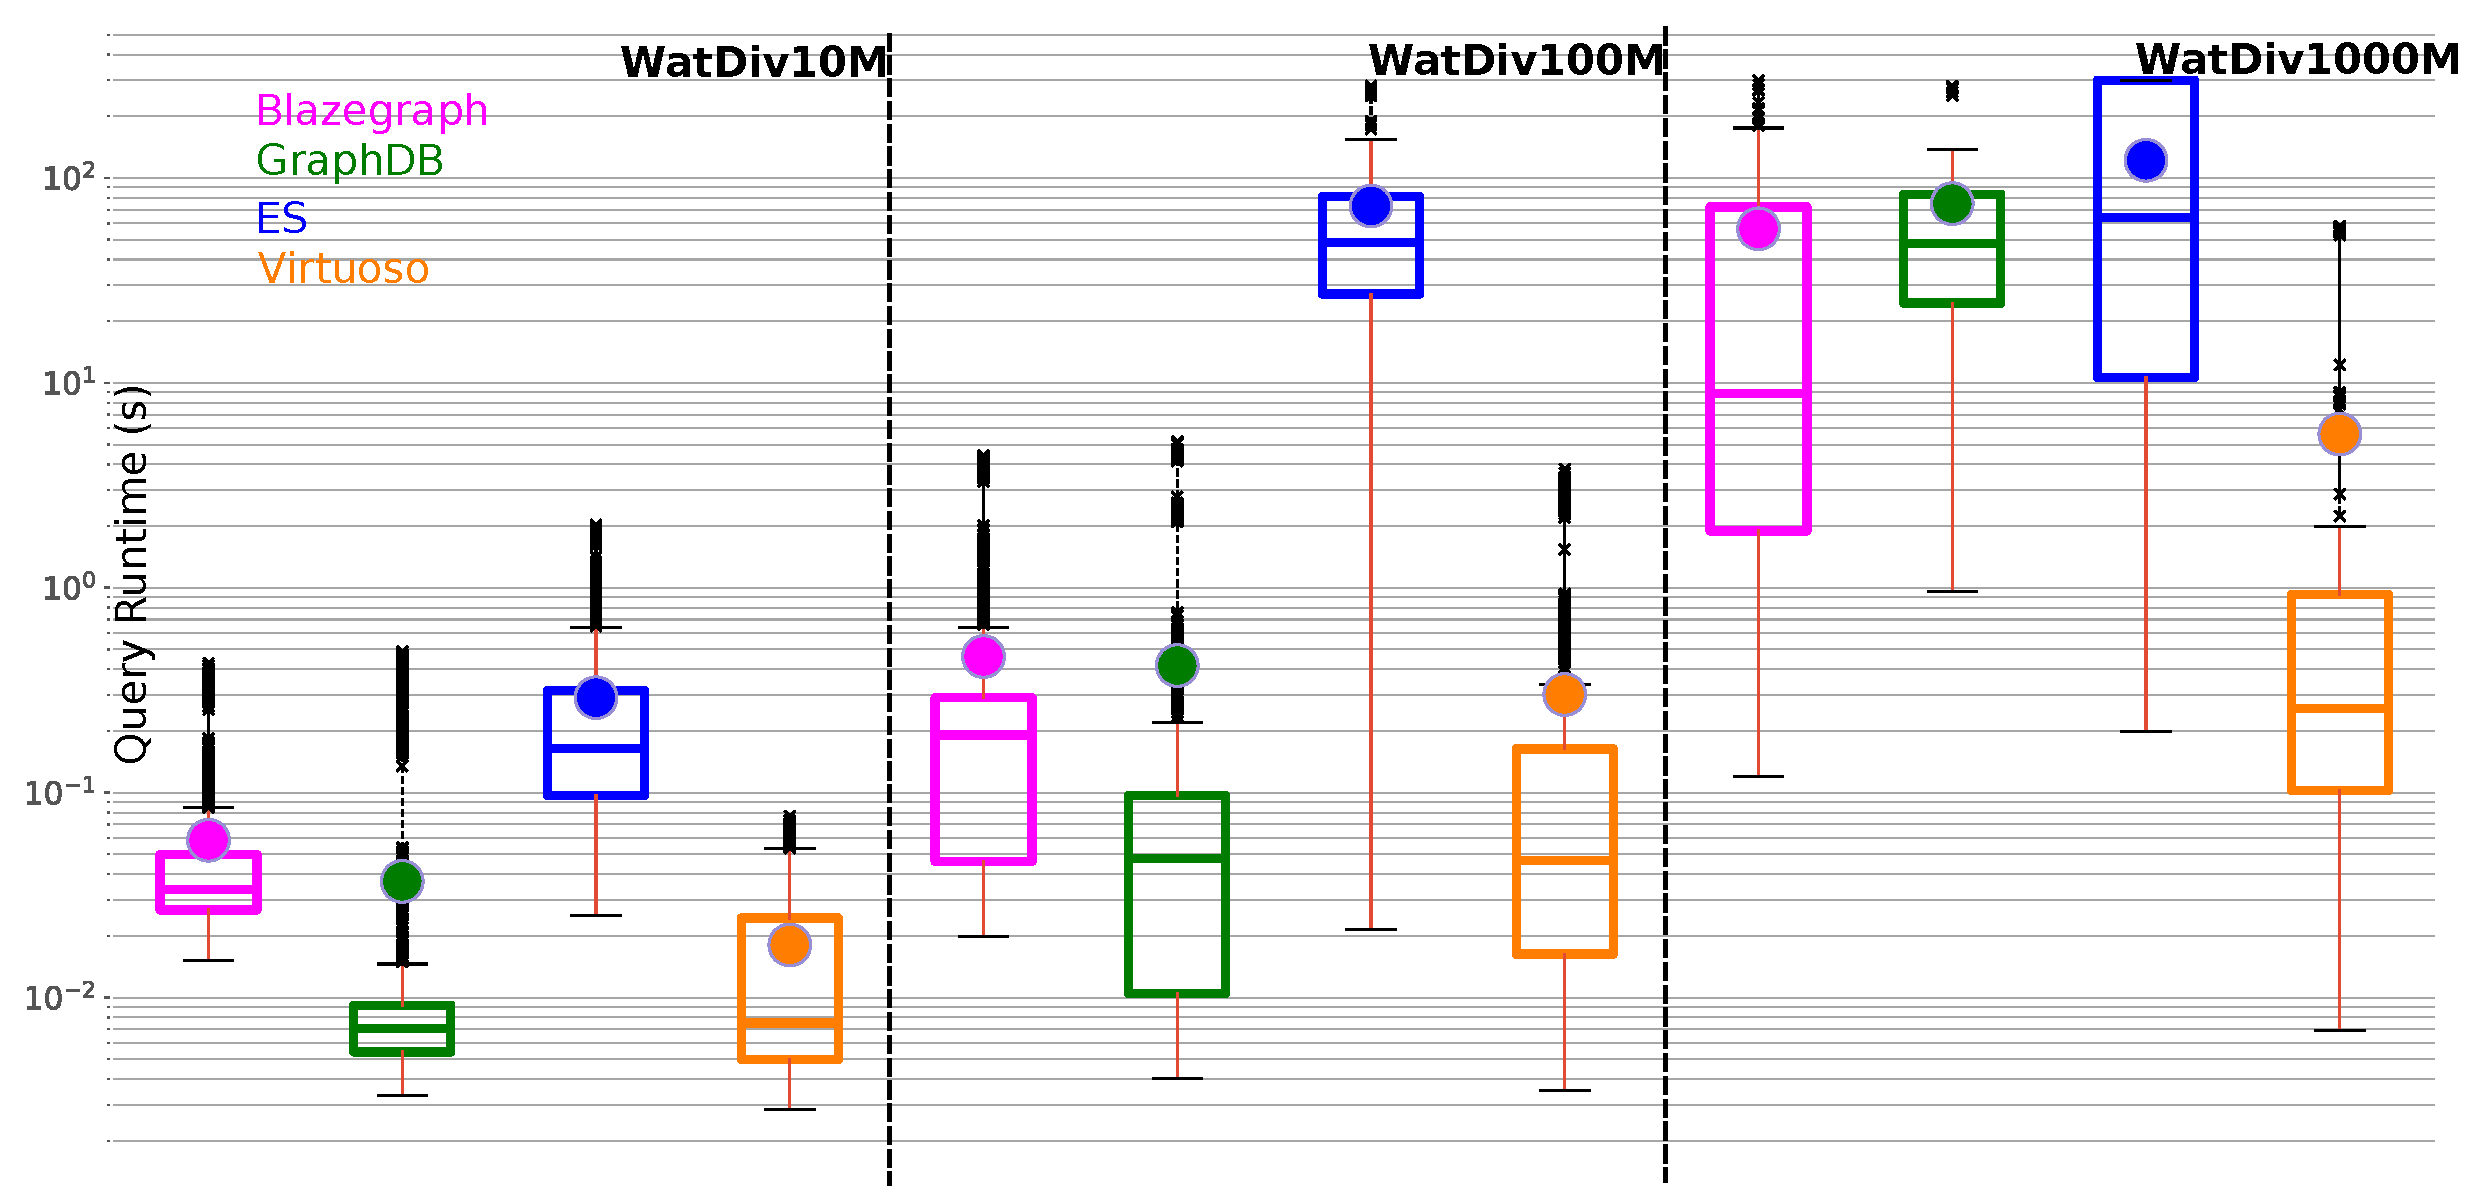
\includegraphics[width=0.9\linewidth]{imgs/Fig01_WatdivNoSQLDataScaling}
	\captionsetup{skip=10pt, font={footnotesize}, labelfont={bf}, width=0.4\textwidth, margin=1cm}
	\caption{ \csentence{Query runtime distributions of \emph{Vendor} systems for 3 different sizes of WatDiv.} Dots correspond to average runtimes, while the horizontal lines in the box plots correspond to median runtimes. The difference is scaling behavior between \textbf{Vir\_32} (linear) and the other stores emphasizes the different impact of server memory on runtime behavior. \textbf{Bla1\_32} and \textbf{Gra1\_32} are very close for batch workloads, for individual queries GraphDB is superior except when scaling up to WatDiv1000M. \textbf{ES1\_32} is the only store with timeout problems starting from WatDiv100M. }
	\label{fig:Fig01_WatdivNoSQLDataScaling}
\end{figure} 
   
%2     
\begin{figure}[ht!]
	\centering
	%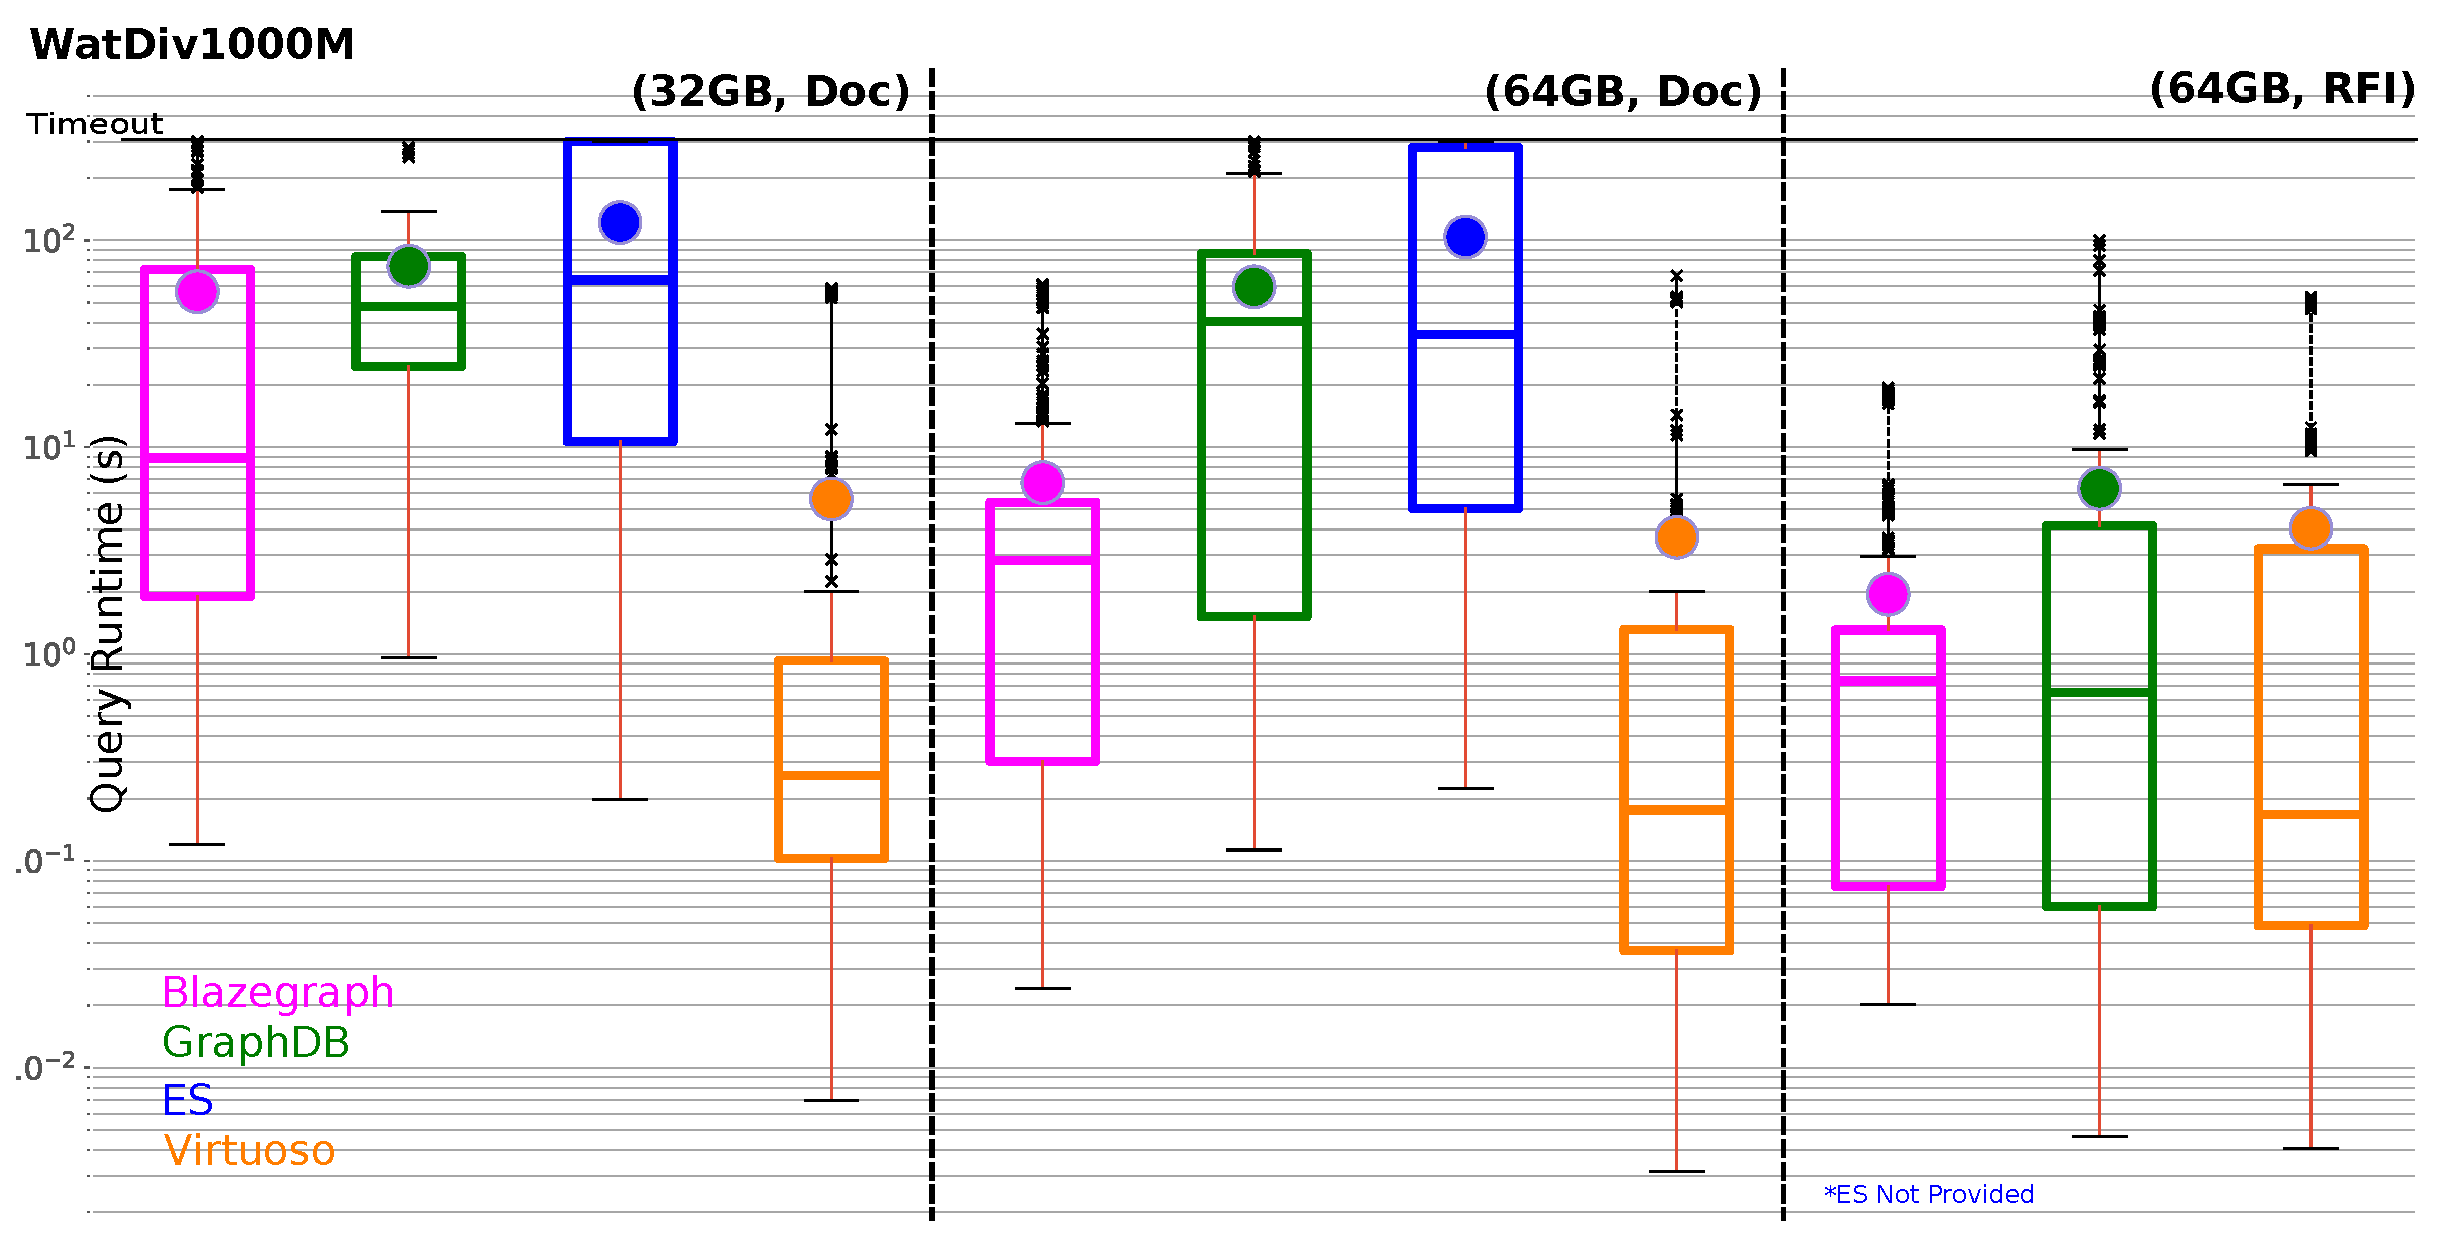
\includegraphics[width=0.9\linewidth]{imgs/Fig02_WatdivVerticalScaling}
	\captionsetup{skip=10pt, font={footnotesize}, labelfont={bf}, width=0.4\textwidth, margin=1cm}
	\caption{\csentence{Query runtime distributions for WatDiv1000M showing the effect of increasing memory from 32GB (left) to 64GB (center) and \emph{Optimized} configurations (right)}. Virtuoso hardly doesn't benefit from additional memory or better configurations. GraphDB is the most sensitive to proper configuration. In the right panel engine performance starts converging. For batch workloads \textbf{Bla1\_64\_Opt} is the fastest, in terms of median runtimes both \textbf{Vir1\_64\_*} setups perform best.}
	\label{fig:Fig02_WatdivVerticalScaling}
\end{figure}

%3      
\begin{figure}[ht!]
	\centering
	%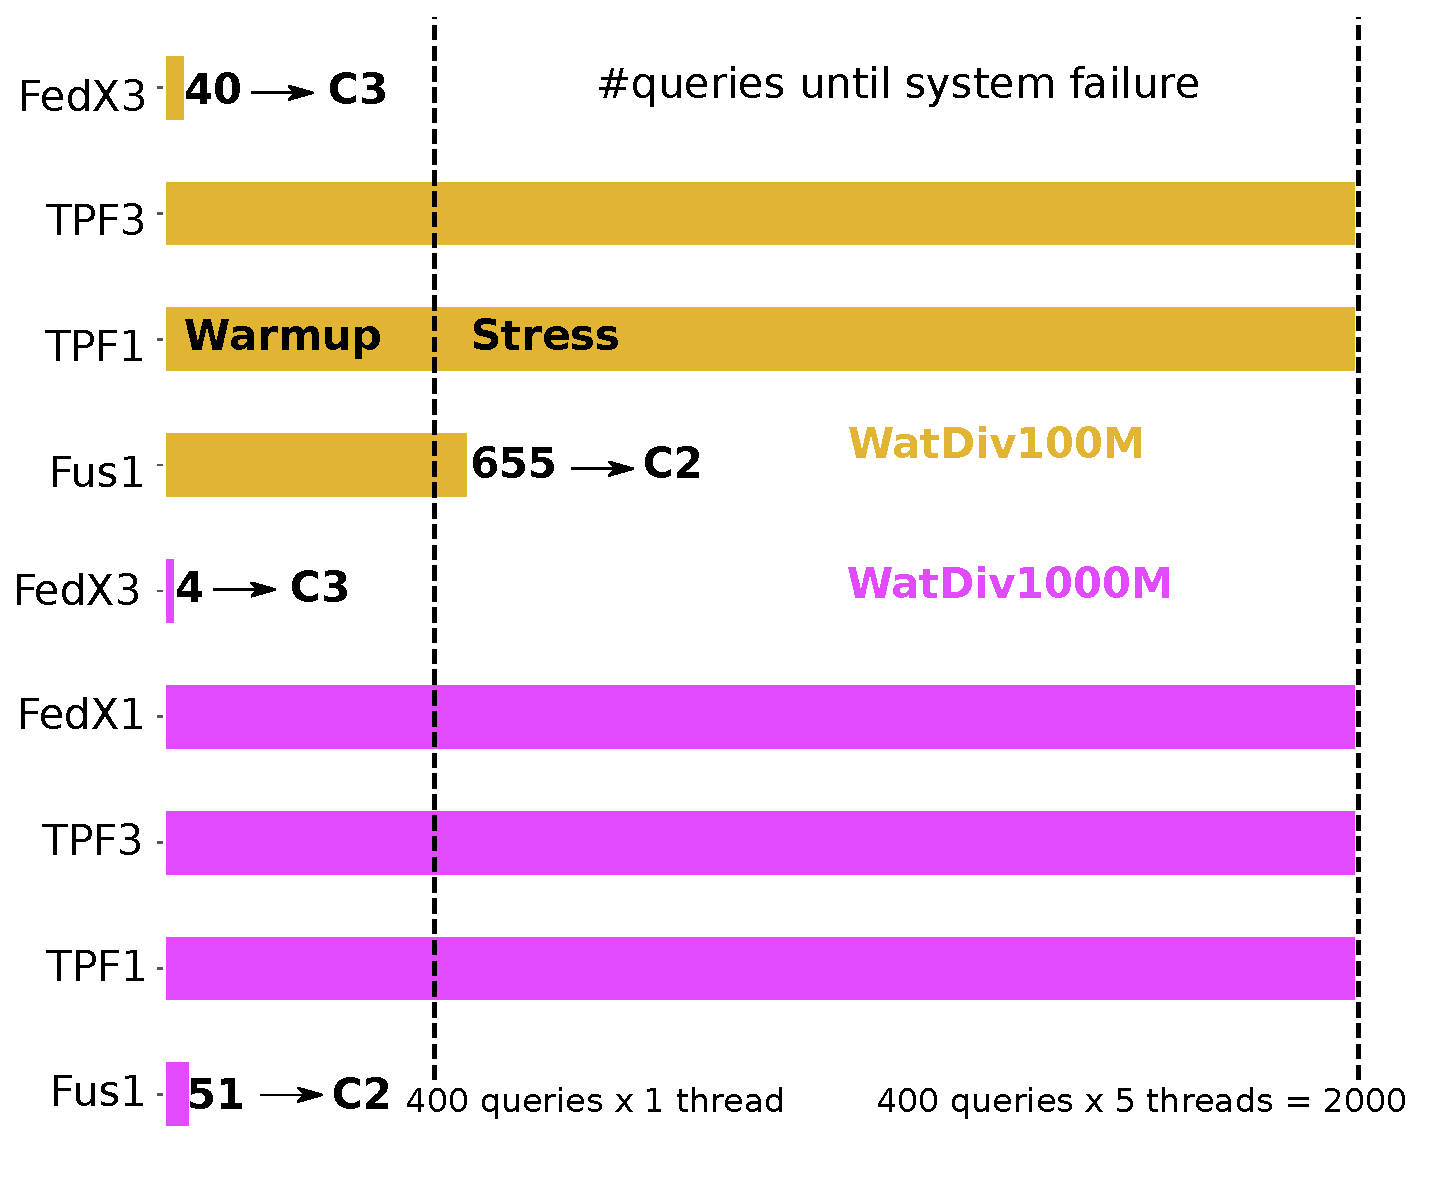
\includegraphics[width=0.99\linewidth]{imgs/Fig03_BenchmarkSurvival_Other_Watdiv_Default}
	\captionsetup{skip=10pt, font={footnotesize}, labelfont={bf}, width=0.4\textwidth, margin=1cm}
	\caption{\csentence{Benchmark survival interval for 3 \emph{SemWeb} solutions}. For early crashes the amount of queries until system failure is reported, as well as the query template causing the failure. \textbf{Flu3\_64} crashes upon the first occurrence of a \textbf{C3} query. \textbf{Fus1\_64} survives the warm-up run for WatDiv100M but crashes upon the first occurrence of a \textbf{C2} query in the stress test, for WatDiv1000M again the first \textbf{C2} query in the warm-up run causes the crash.}
	\label{fig:Fig03_BenchmarkSurvival_Other_Watdiv_Default}
\end{figure}   

%4
\begin{figure}[ht!]
	\centering
	%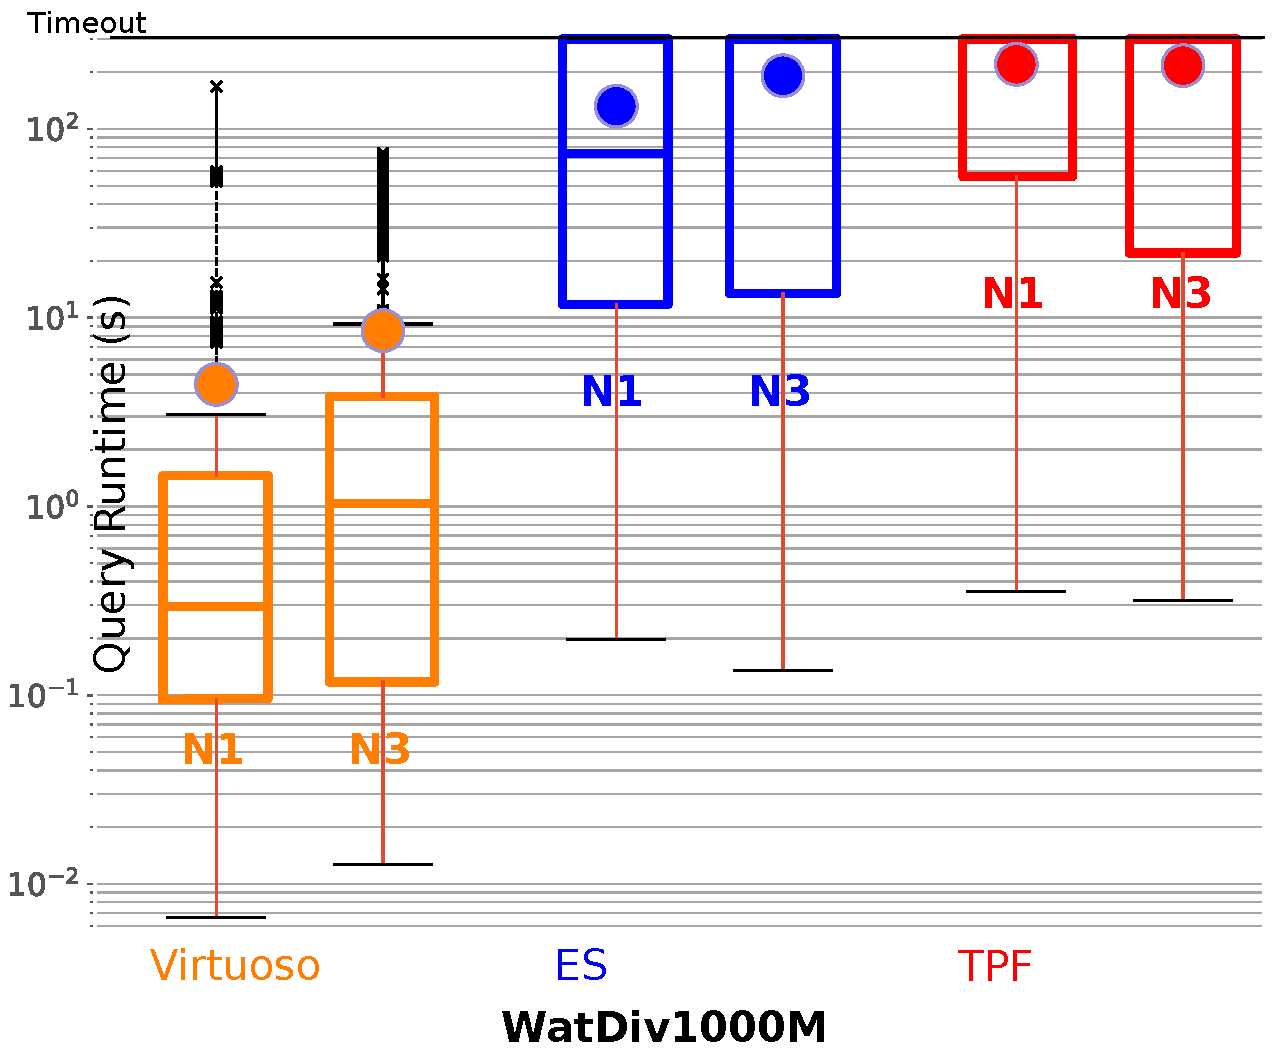
\includegraphics[width=0.9\linewidth]{imgs/Fig04_WatdivHorizontalScaling}
	\captionsetup{skip=10pt, font={footnotesize}, labelfont={bf}, width=0.4\textwidth, margin=1cm}
	\caption{\csentence{Pairwise comparison of query runtime distributions for single-node versus 3-node setups}. None of the solutions achieve an average runtime speedup when adding more nodes, on the contrary overhead multipication factors of 1.9 and 1.5 are seen in left and center pane for \textbf{Vir3\_32\_Def} and \textbf{ES3\_32\_Def}. For \textbf{TPF3\_64\_Def} the overhead is negligible.}
	\label{fig:Fig04_WatdivHorizontalScaling}
\end{figure}

%5
\begin{figure}[ht!]
	\centering
	%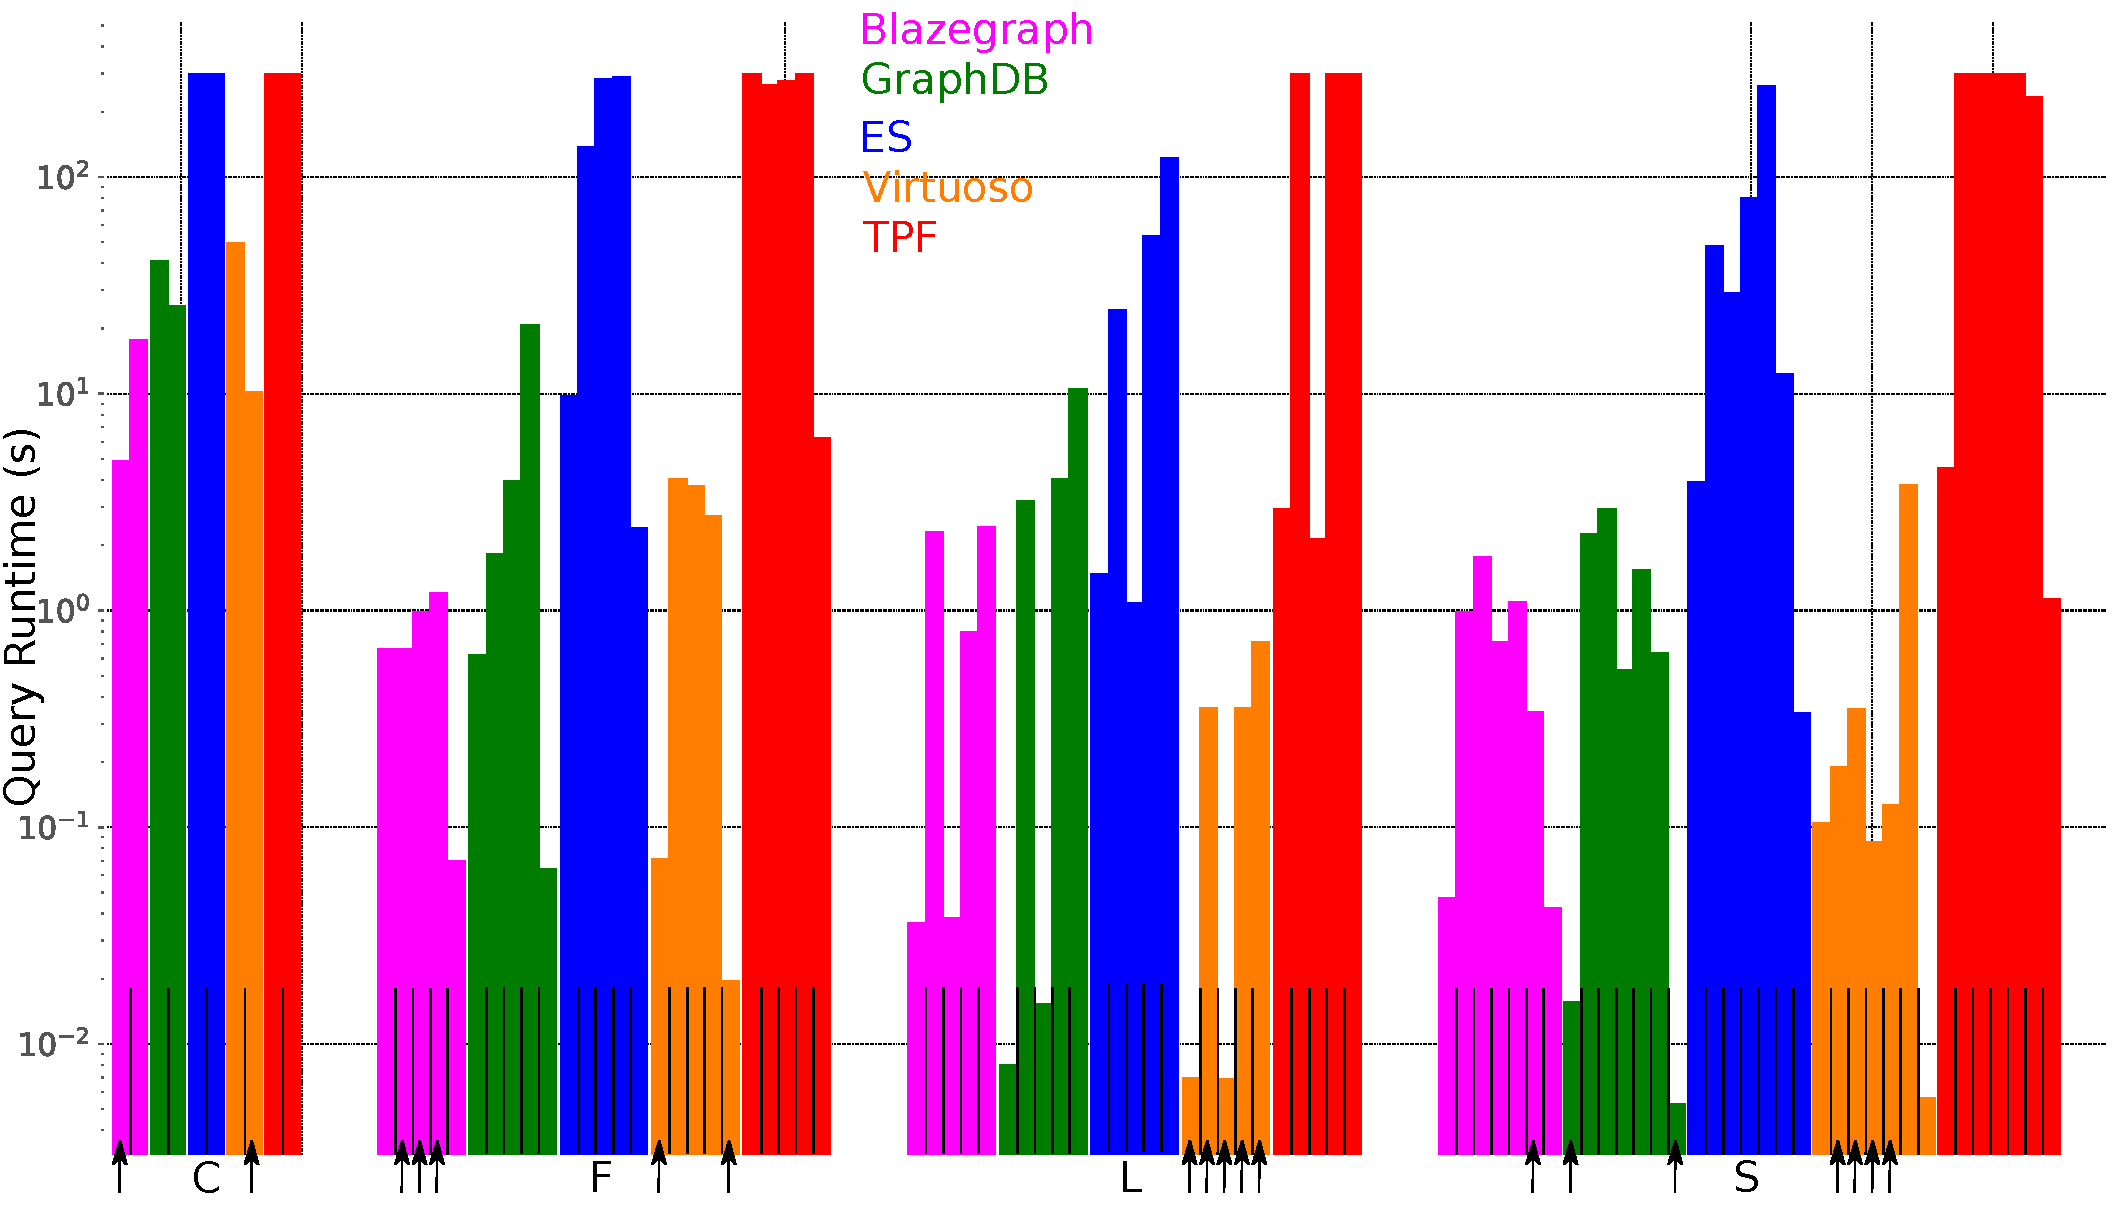
\includegraphics[width=0.9\linewidth]{imgs/Fig05_WatdivTemplates}
	\captionsetup{skip=10pt, font={footnotesize}, labelfont={bf}, width=0.4\textwidth, margin=1cm}
	\caption{\csentence{Average Runtime per query template for 5 single-node setups.} \textbf{TPF1\_64} has only 5 templates which do not coincide with the timeout of 300s, for \textbf{ES1\_64\_Def} this is alread 15 templates.
		\textbf{Vir1\_64\_Opt} is the fastest engine for 13 templates, \textbf{Gra1\_64\_Opt} for and \textbf{Bla1\_64\_Opt} for 3 templates each. Template \textbf{C3} was omitted due to query completeness issues. Blazegraph was the only engine to retrieve all results. } 
	\label{fig:Fig05_WatdivTemplates}
\end{figure}
 
%6
\begin{figure}[ht!]
	\centering
 	%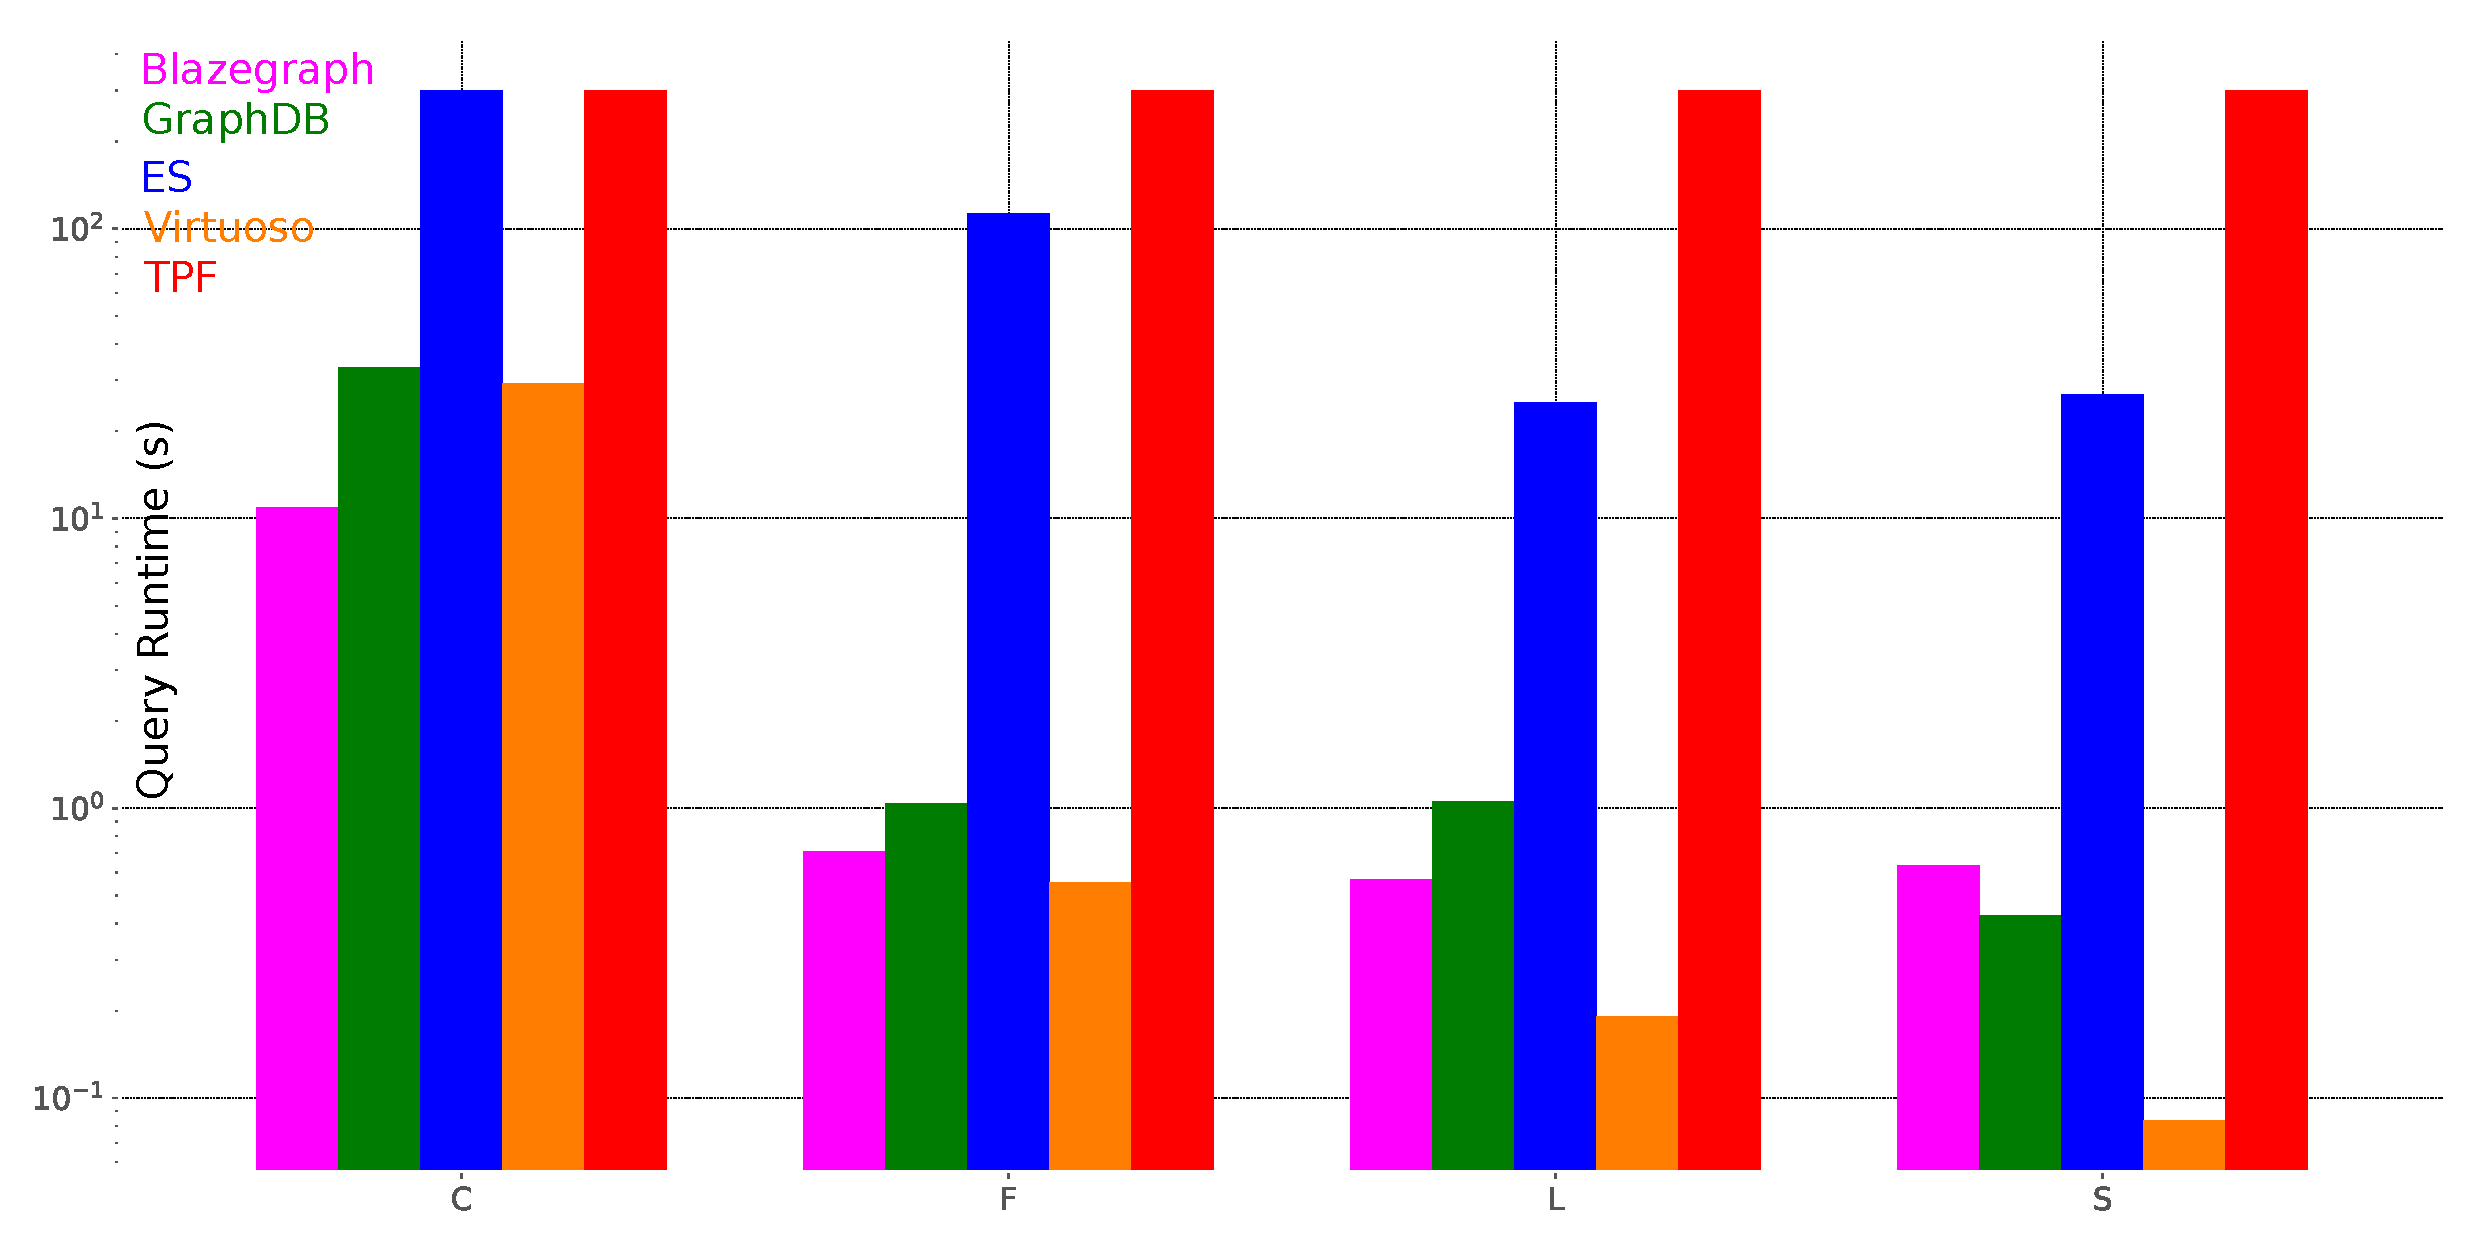
\includegraphics[width=0.9\linewidth]{imgs/Fig06_WatdivTemplateTypes}
 	\captionsetup{skip=10pt, font={footnotesize}, labelfont={bf}, width=0.4\textwidth, margin=1cm}
 	\caption{\csentence{Average Runtime per BGP type.}}
 	\label{fig:Fig06_WatdivTemplateTypes}
\end{figure}
   
%7   
\begin{figure}[ht!]
	\centering
	%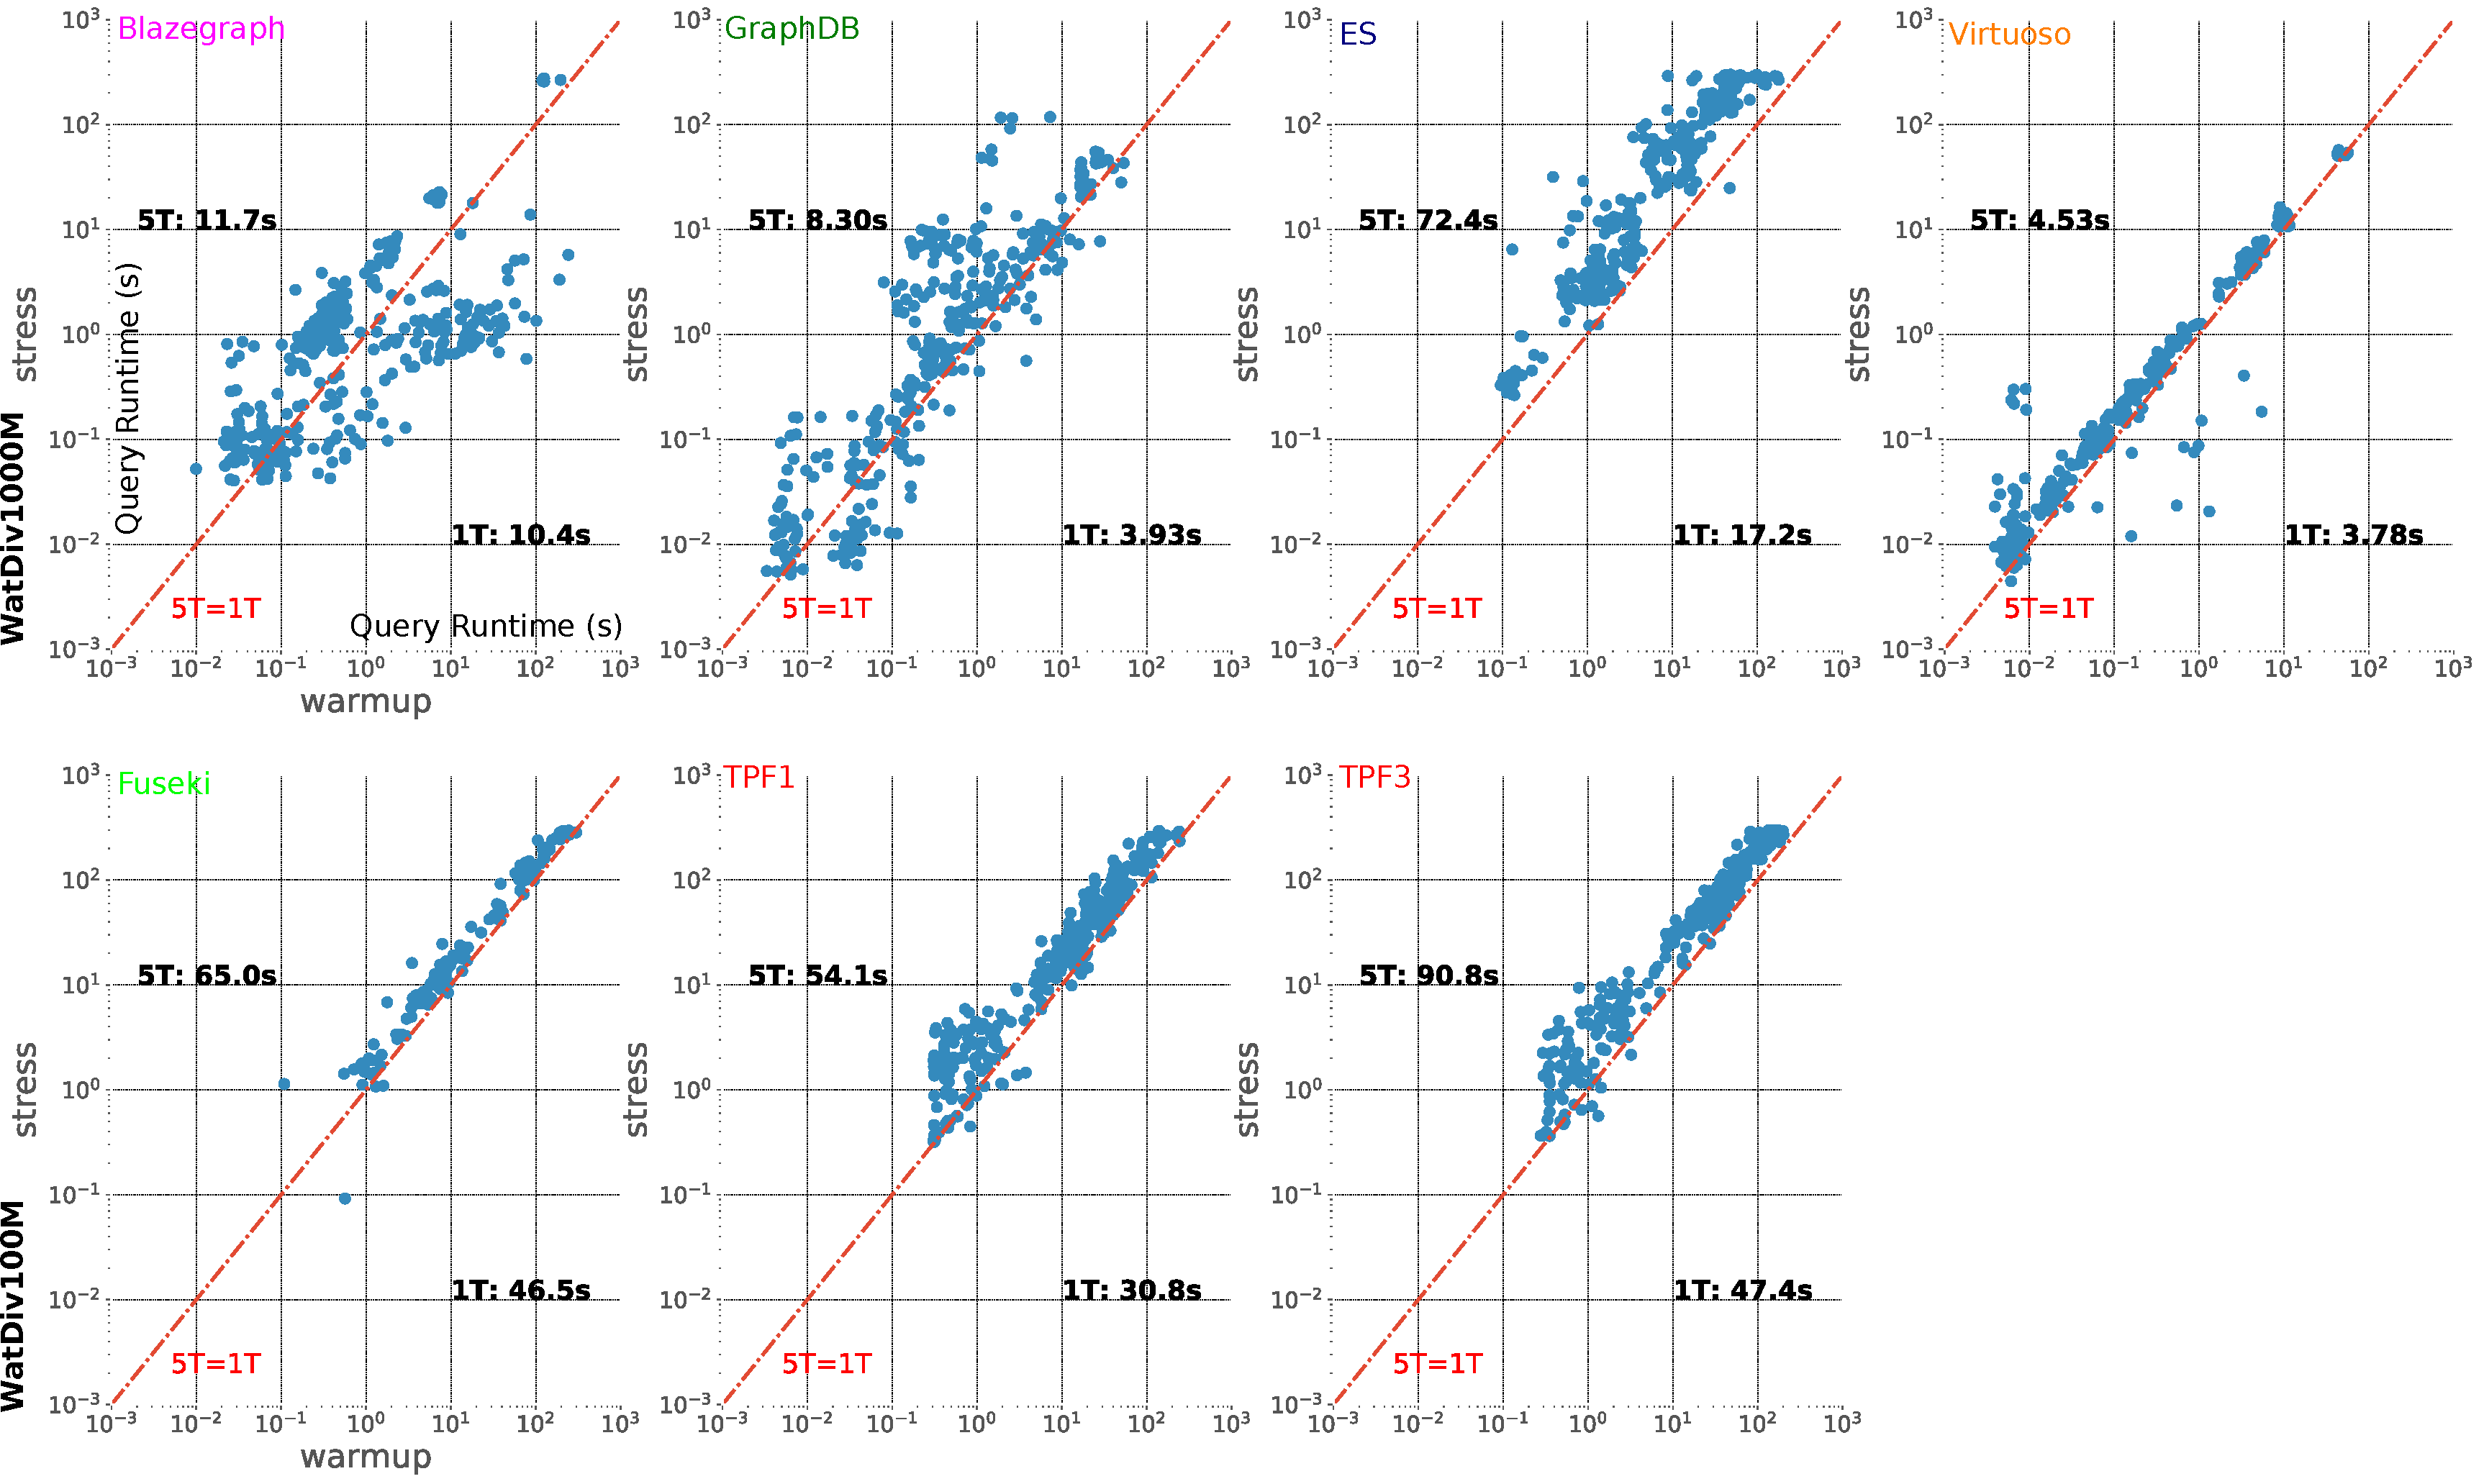
\includegraphics[width=0.90\linewidth]{imgs/Fig07_Watdiv_SingleMultiClient}
	\captionsetup{skip=10pt, font={footnotesize}, labelfont={bf}, width=0.4\textwidth, margin=1cm}
	\caption{\csentence{Runtimes for single versus multi-client workloads: 1 vs. 5 threads.} 
		5T runtime corresponds to the maximum runtime per query in the stress test, 1T is the runtime during the warm-up phase. The red line corresponds to the bisector, where the runtime for both workloads is equal. Dots are expected to be shifted up, which correspond to a multiplication factor. The closer the dots to the bisector the smaller the multi-client overhead. Dots below the bisector can be attributed to the natural variance in query runtimes. Average runtimes per store are also shown. \textbf{Bla1\_64} and \textbf{Vir1\_64} have the smallest overhead $(< 20\%)$, for \textbf{ES1\_64} has the largest $(> 300\%)$.
	}
	\label{fig:Fig07_Watdiv_SingleMultiClient}
\end{figure}

%8
\begin{figure}[ht!]
	\centering
	%\includegraphics[width=0.9\linewidth]{imgs/Fig08_Watdiv_caching}
	\captionsetup{skip=10pt, font={footnotesize}, labelfont={bf}, width=0.4\textwidth, margin=1cm}
	\caption{\csentence{Speedup in query runtime.} We compare query runtimes in the multi-threaded run with the slowest execution in the stress test. With no caching all dots are expected on the X and Y-axis, the latter because of the noise on small query runtimes. If we focus on speedups $> 2$, especially \textbf{ES1} and \textbf{TPF*} seem to have the highest benefit.  }
	\label{fig:Fig08_Watdiv_caching}
\end{figure}

%9
\begin{figure}[ht!]
	\centering
	%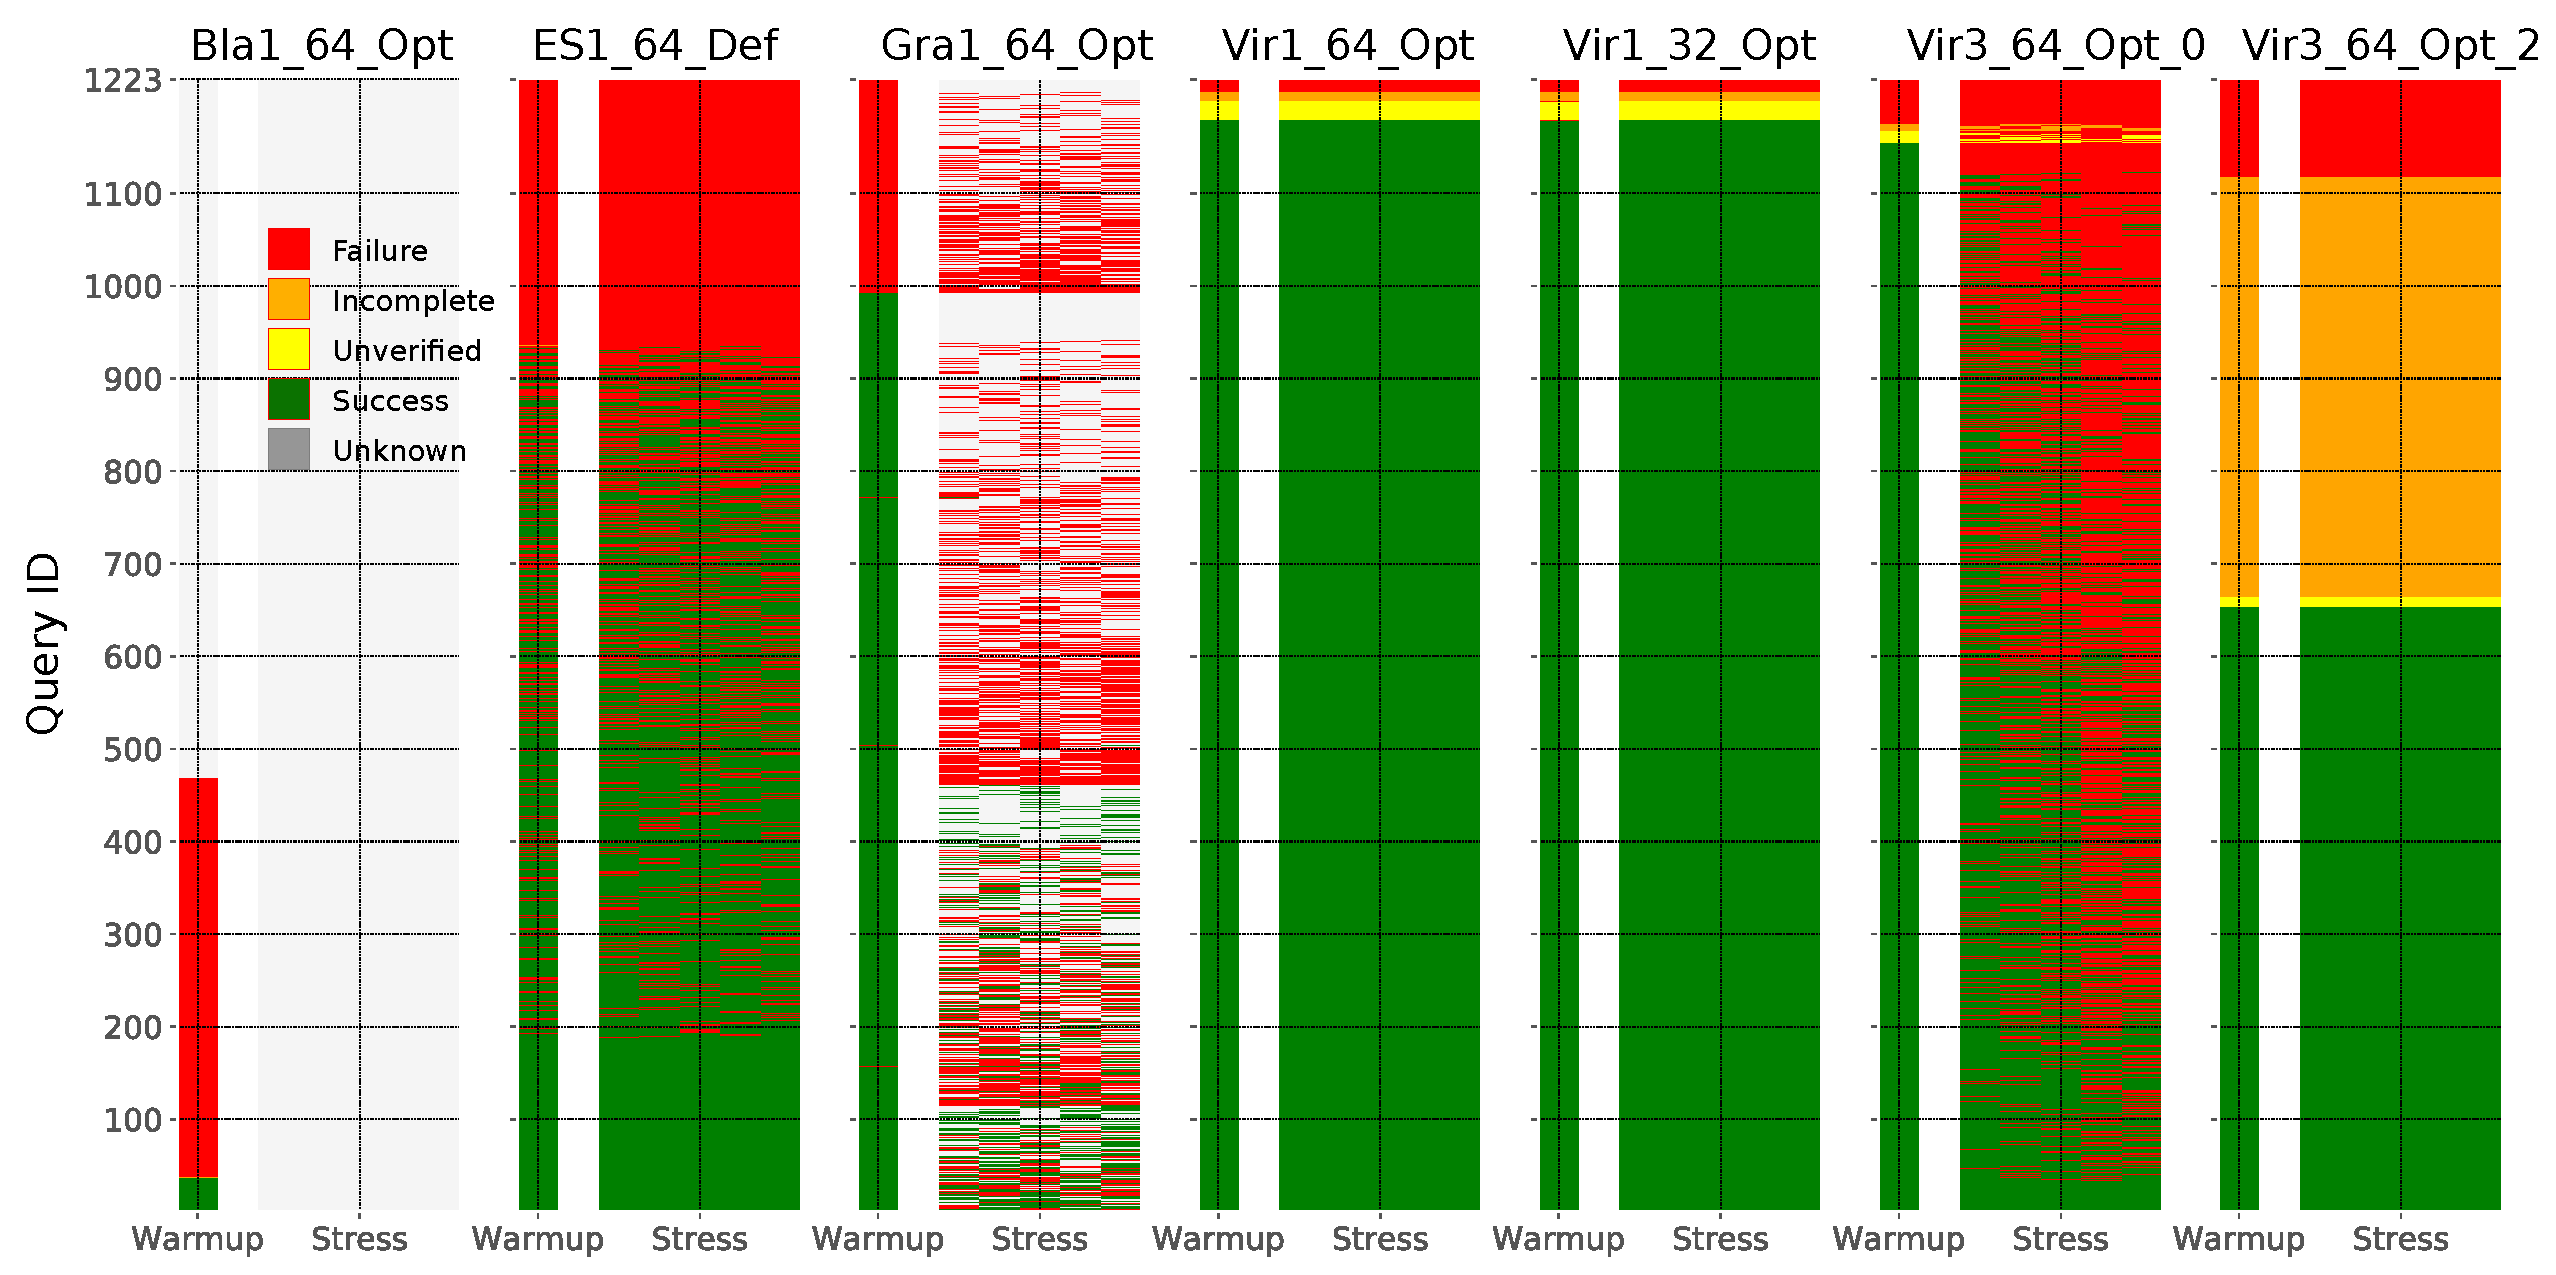
\includegraphics[width=0.90\linewidth]{imgs/Fig09_FailuresOntoforceBM}
	\captionsetup{skip=10pt, font={footnotesize}, labelfont={bf}, width=0.4\textwidth, margin=1cm}
	\caption{\csentence{Overview of successes and errors per query (Y-axis) and thread (X-axis) on the Ontoforce benchmark.}
		Queries are sorted per system in order to group error behavior and are not consistent between simulations!
		Blazegraph has a short benchmark survival interval. \textbf{ES1}, \textbf{Gra1} and \textbf{Vir3} Cluster setups have a lot of errors but most queries execute successfully at least once, which allows runtime comparisons. \textbf{Vir3\_64\_Opt\_0} is the most successful Virtuoso cluster run as query completeness analysis revealed that \textbf{Vir3\_64\_Opt\_2} has unreported errors for 37\% of the queries.
	}
	\label{fig:Fig09_FailuresOntoforceBM}
\end{figure}   

%10
\begin{figure}[ht!]
	\centering
	%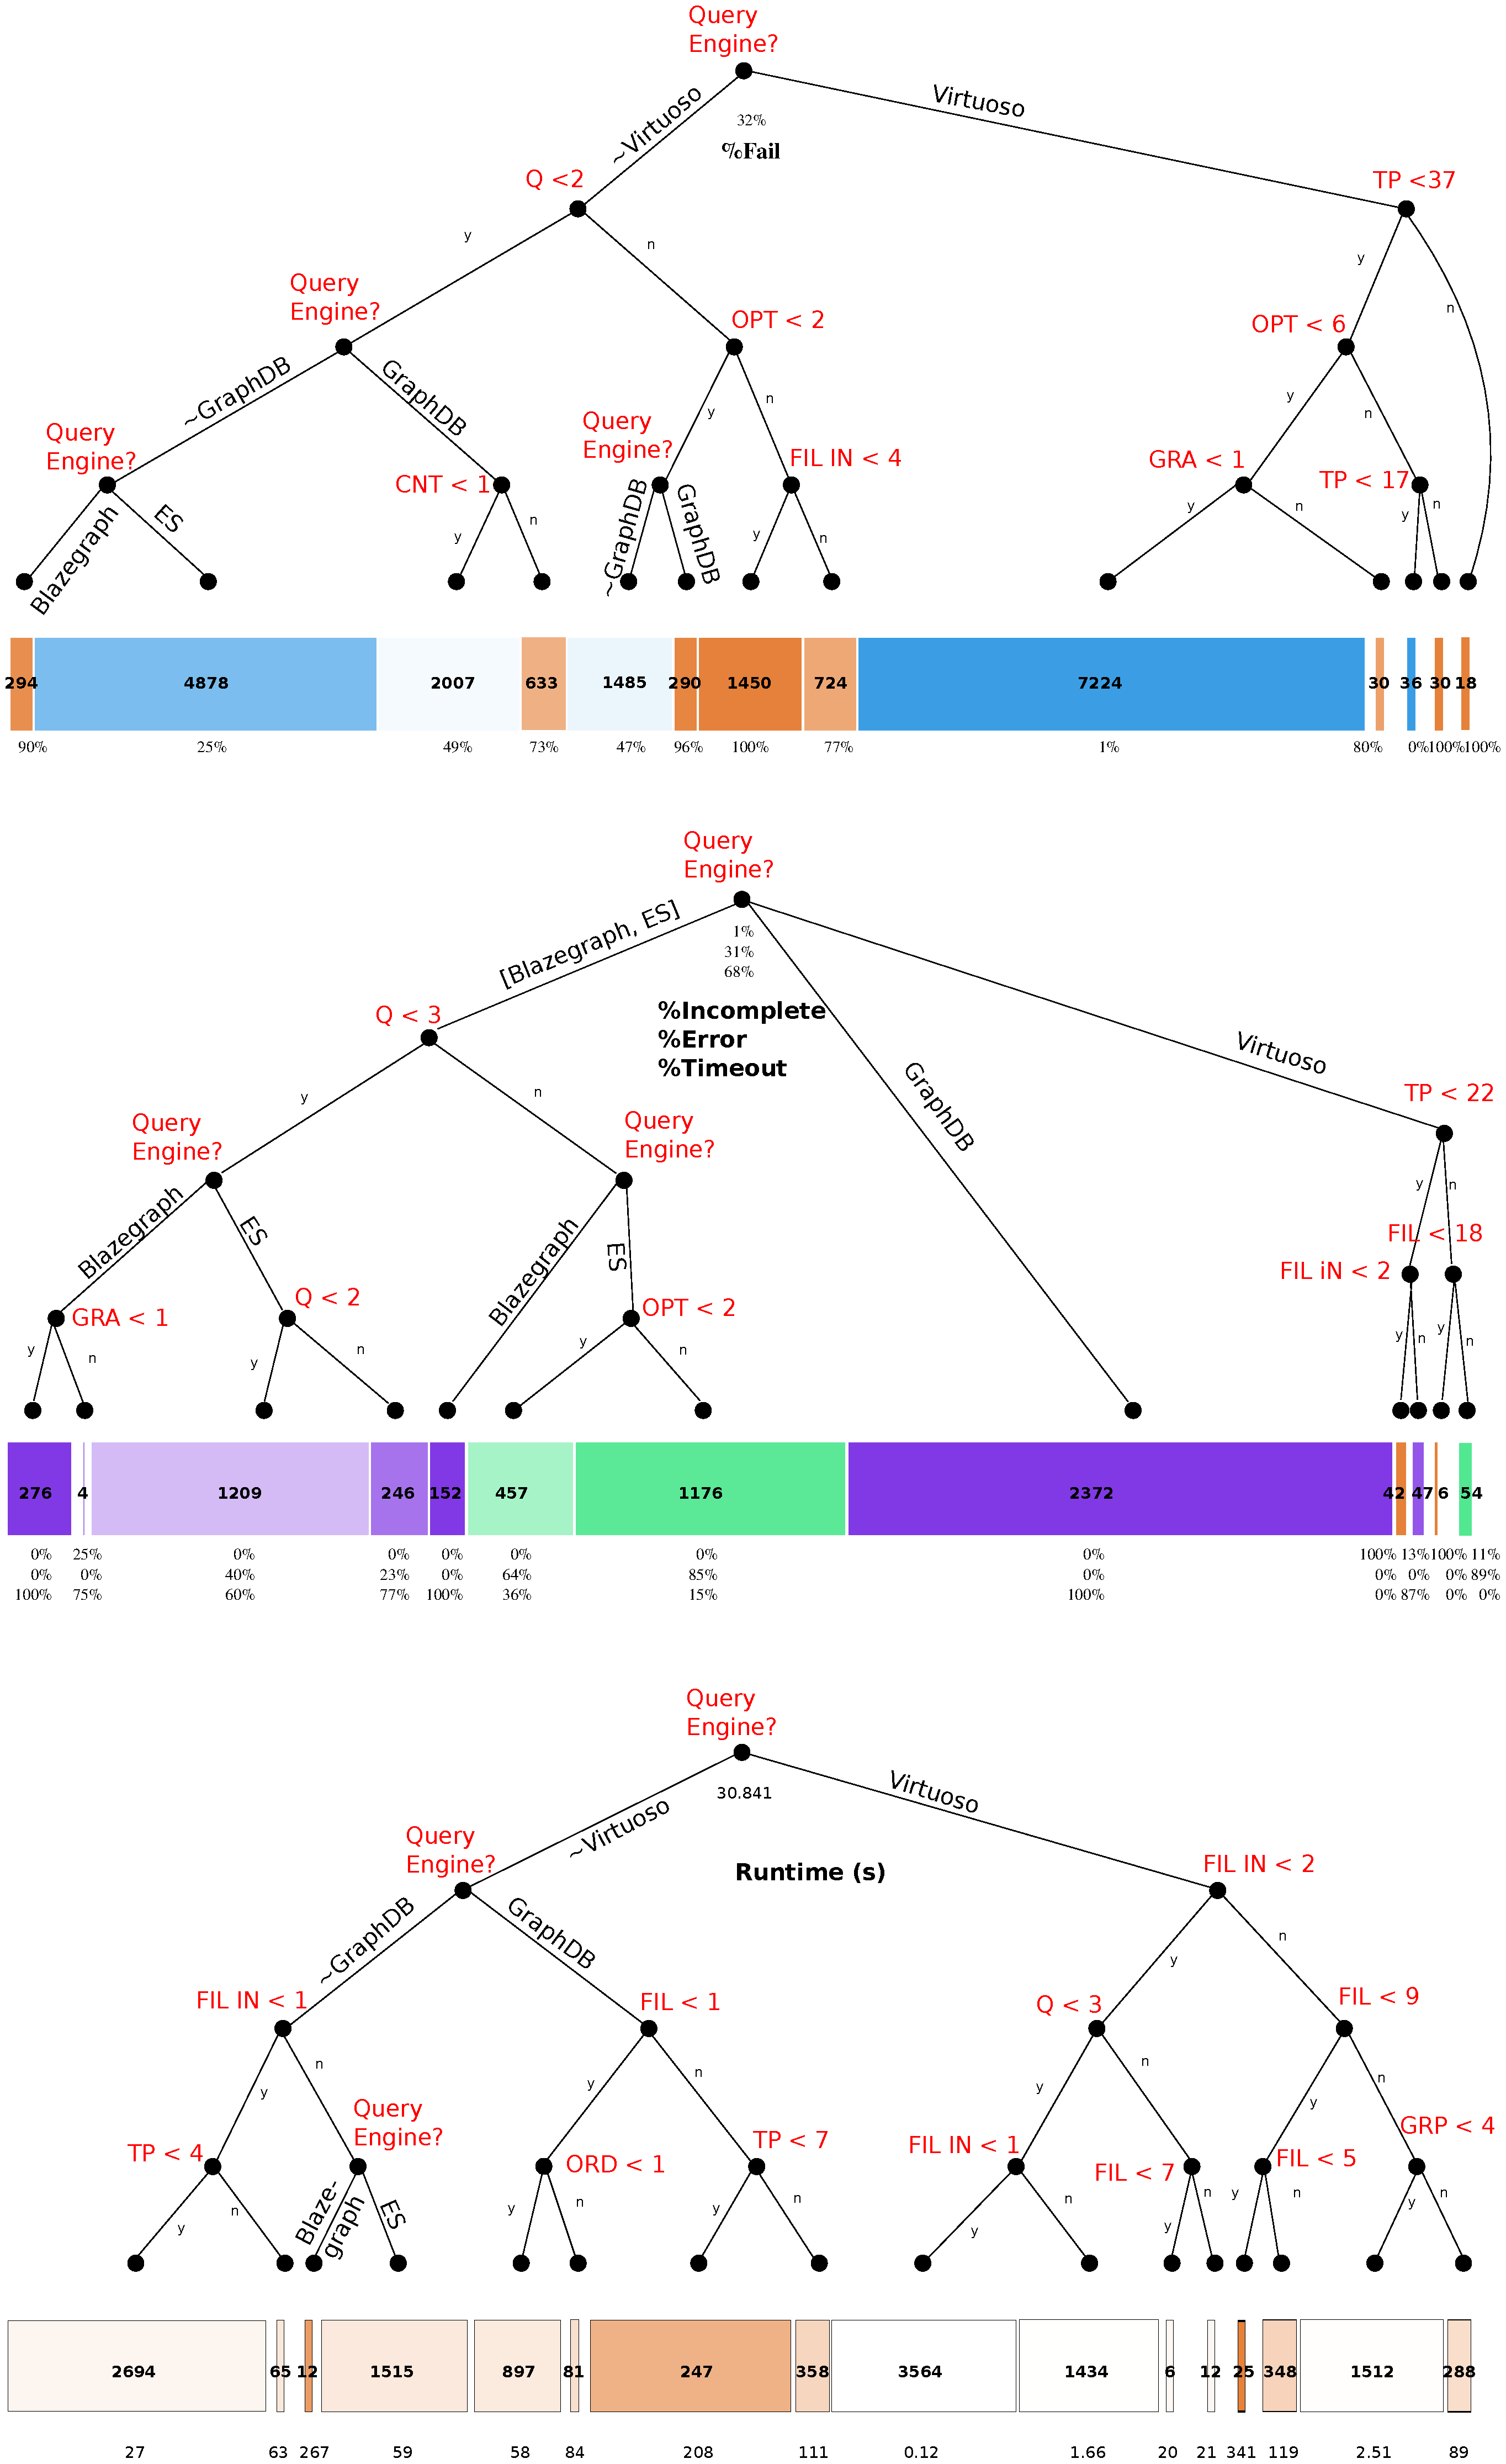
\includegraphics[width=0.75\linewidth]{imgs/Fig10_AllTrees}
	\captionsetup{skip=10pt, font={footnotesize}, labelfont={bf}, width=0.4\textwidth, margin=1cm}
	\caption{\csentence{Decision Tree Analysis to identify the reason for query failure, certain error types, and high/low query runtimes.} Input for all trees are feature vectors, also the query engine is added as a categorical feature. Rules in the decision trees are shown in red, sample sizes are encoded as the width of the bottom bar and the value is added inside the bars in bold. For each separate part the class distribution or the average runtime is reported below the bar. 
		\newline \hspace{\linewidth} 	
		\underline{\smash{Top:}} Classification into query success (blue) and failure (red) and incomplete. The query engine is an important decision rule, which demonstrates that Virtuoso behaves very different from the other systems.  
		\newline \hspace{\linewidth} 	
		\underline{\smash{Center:}} Classification of query failures into classes incomplete (orange), server error (green), and timeout (purple). 
		\newline \hspace{\linewidth} 	
		\underline{\smash{Bottom:}}  Regression on query runtimes. Red corresponds to high query runtimes, white to low. }
	\label{fig:Fig10_AllTrees}
\end{figure}

%11
\begin{figure}[ht!]
	\centering
	%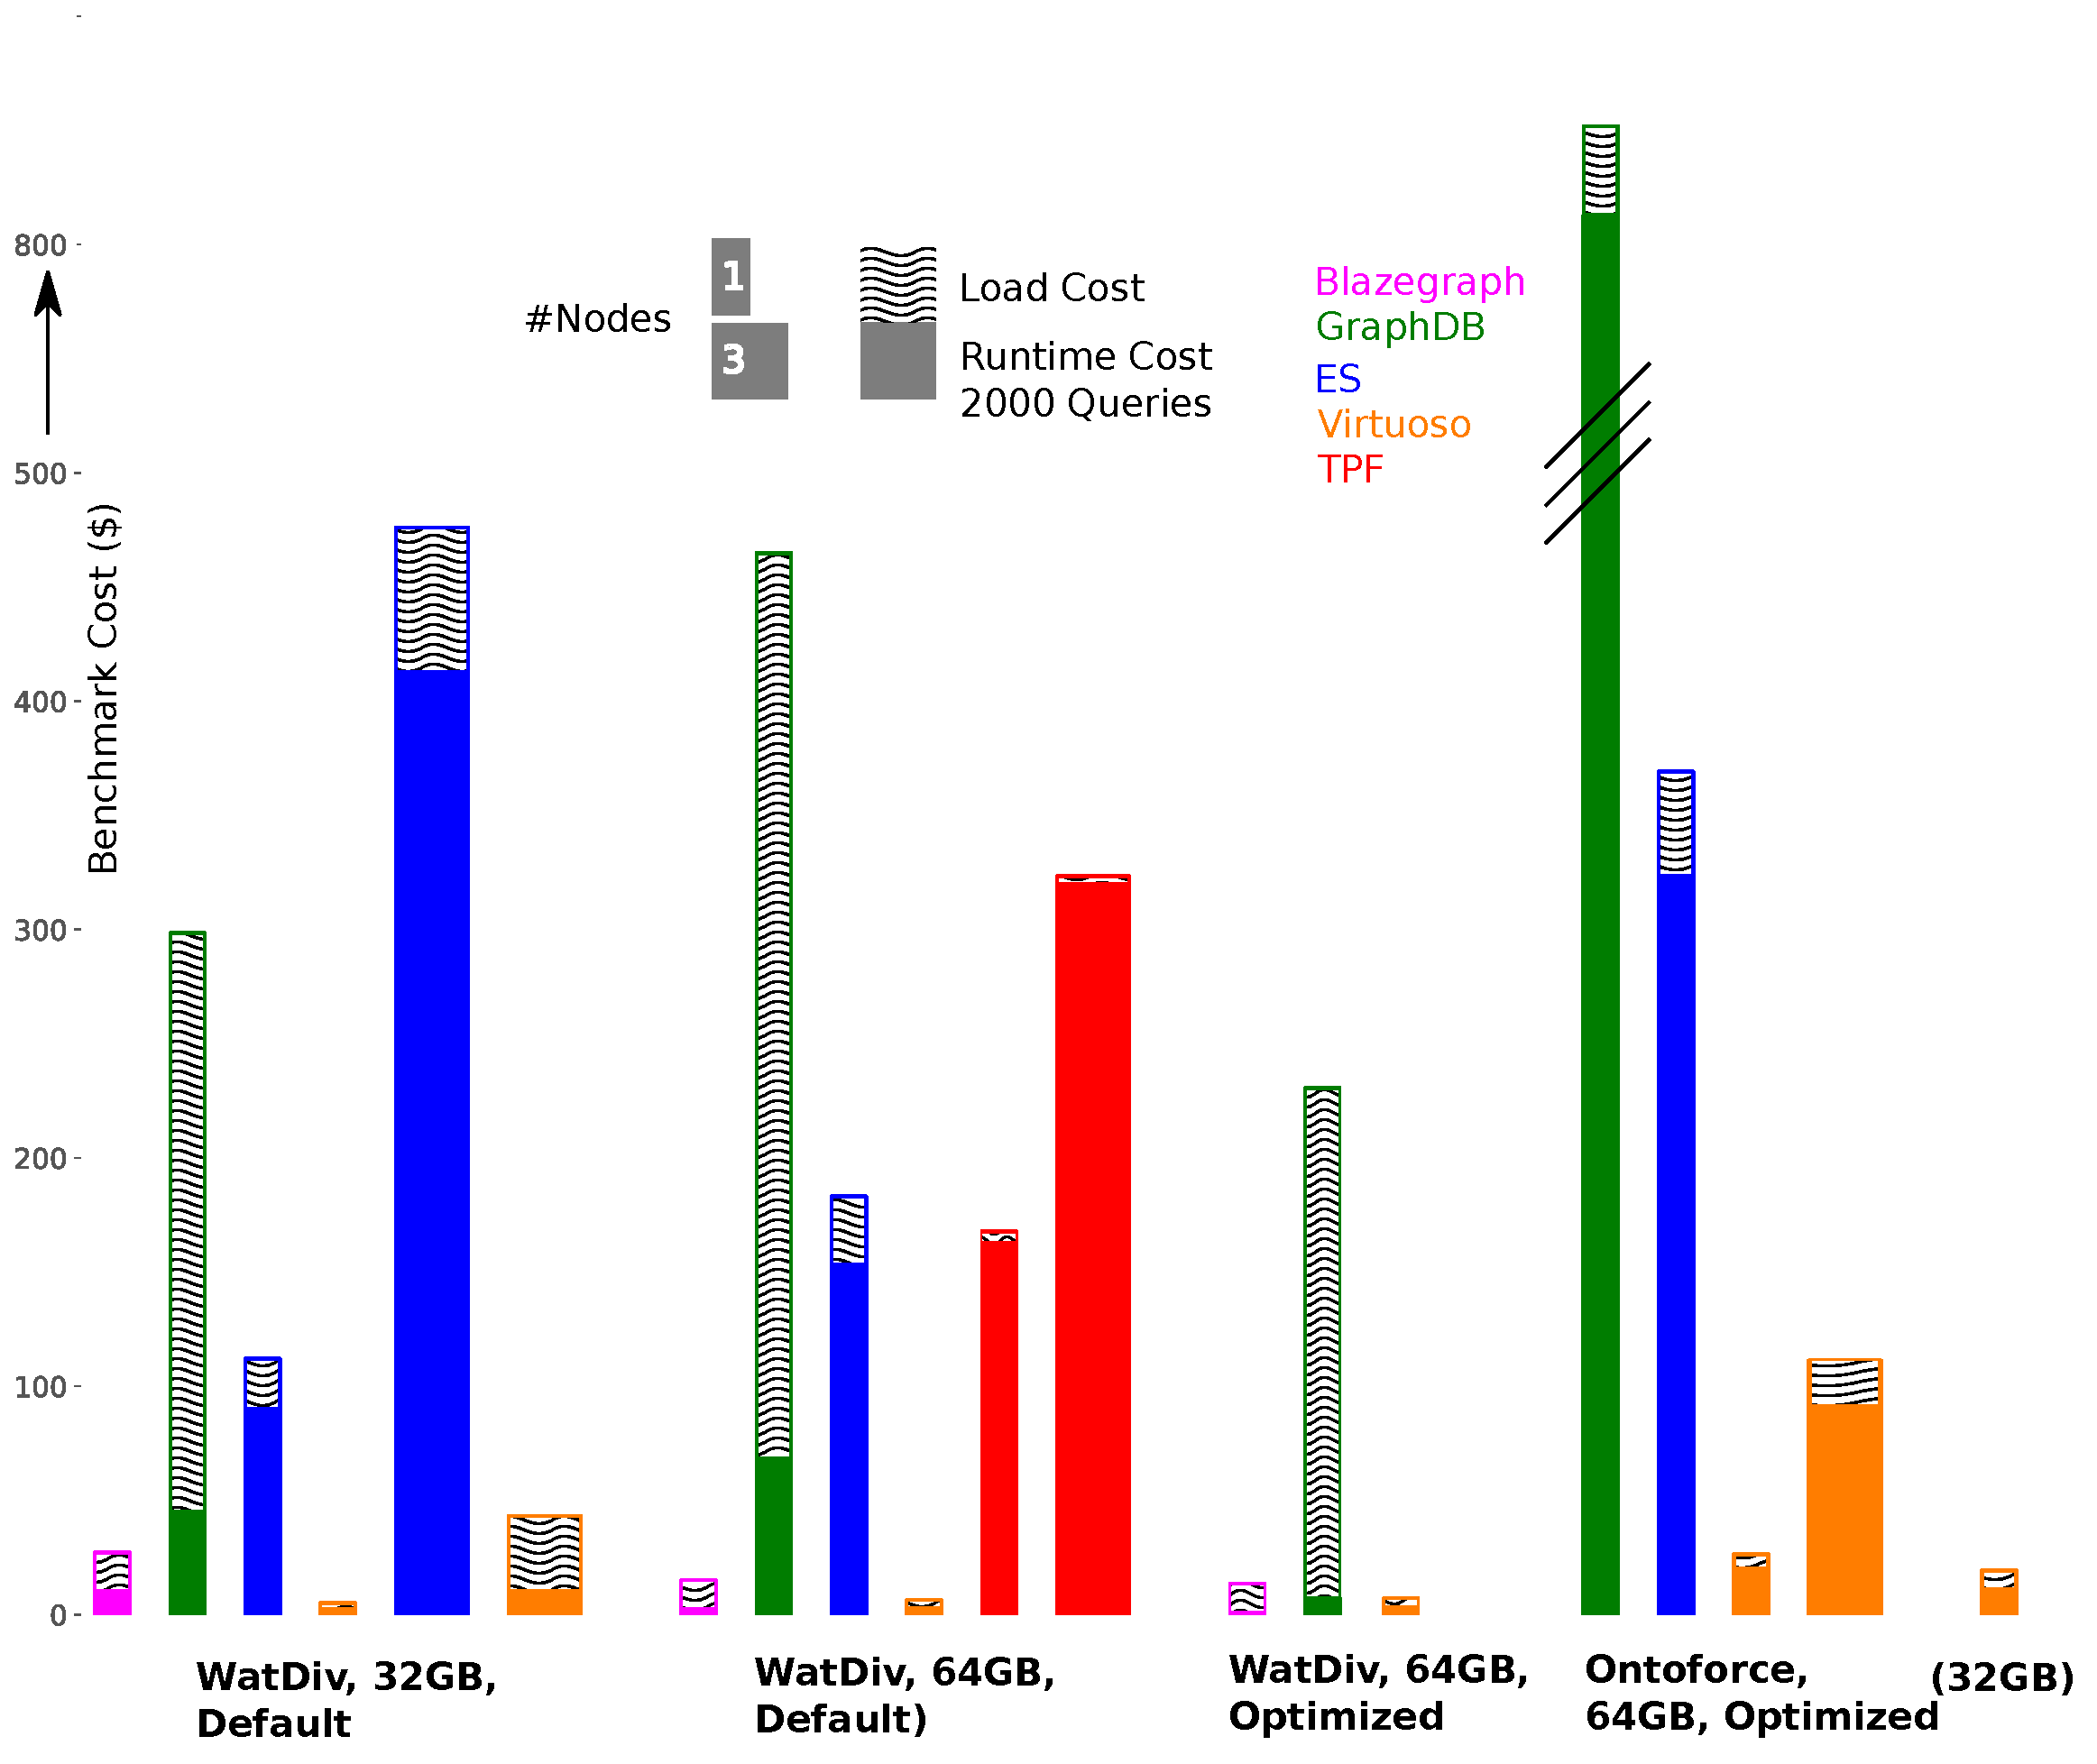
\includegraphics[width=0.9\linewidth]{imgs/Fig11_AllSims_Correct}
	\captionsetup{skip=10pt, font={footnotesize}, labelfont={bf}, width=0.4\textwidth, margin=1cm}
	\caption{\csentence{Benchmark Cost in \$ to load and execute 2000 queries in a stress test for WatDiv1000M or Ontoforce datasets for different setups.} All stacked bars consists the load cost stacked on top of the runtime cost. Bar width encodes the amount of nodes. For WatDiv \textbf{Vir1\_32\_Def} is the least expensive solution, mainly because \textbf{Bla1\_64\_Opt} has a much higher load cost. Also for the Ontoforce benchmark\textbf{ Vir1\_32\_Opt} is the most cost-effective choice. The engine ranking is not conserved going from artificial to real-world benchmark.}
	\label{fig:Fig11_AllSims_Correct}
\end{figure}

%%%%%%%%%%%%%%%%%%%%%%%%%%%%%%%%%%%
%%                               %%
%% Tables                        %%
%%                               %%
%%%%%%%%%%%%%%%%%%%%%%%%%%%%%%%%%%%

%% Use of \listoftables is discouraged.
%%
%\section*{Tables}
%\begin{table}[h!]
%\caption{Sample table title. This is where the description of the table should go.}
%      \begin{tabular}{cccc}
%        \hline
%           & B1  &B2   & B3\\ \hline
%        A1 & 0.1 & 0.2 & 0.3\\
%        A2 & ... & ..  & .\\
%        A3 & ..  & .   & .\\ \hline
%      \end{tabular}
%\caption*{Text below}
%\end{table}

%%%%%%%%%%%%%%%%%%%%%%%%%%%%%%%%%%%
%%                               %%
%% Additional Files              %%
%%                               %%
%%%%%%%%%%%%%%%%%%%%%%%%%%%%%%%%%%%

\section*{Additional Files}
  \subsection*{Sequel Project Website}
    The website links to all material related to this manuscript: datasets, notebooks with analysis, raw log files,\ldots can be found here: \url{http://users.elis.ugent.be/~drdwitte/index.html}

  \subsection*{Feature Matrix}
  Overview om Semantic Databases considered in this benchmark with together with a set of
  features and links where this information was found:   \url{http://users.elis.ugent.be/~drdwitte/featurematrix.html}
  \subsection*{Notebooks and CSV files for postprocessing}
  All CSV files with different views on the benchmark output together with the Jupyter notebook files showing the original analysis of the data can be found here: \url{http://users.elis.ugent.be/~drdwitte/postprocessing.html}
\end{backmatter}
\end{document}
